% 	Modelo de Tese/Dissertação segundo as normas da Pós-graduação do IFSC-USP
% 	Criado por Alexandre de Castro Maciel - Grupo de Polimeros Bernhard Gross
% 	Este trabalho está licenciado sob uma Licença Creative Commons Atribuição-Uso Não-Comercial-Compartilhamento pela mesma Licença 2.5 Brasil
% 	Modelo criado e testado em ambiente Linux/Debian
% 	Software utilizados: Kile,Kbibtex,Kpdf,Gimp
%
%
\newcommand{\massa}{{\large \textsc{massa}}}
\newcommand{\mass}{{\large \textsc{mass}}}
\newcommand{\figgus}{{\large \textsc{figgus}}}

%-----------------TIPO DE DOCUMENTO------------------
\documentclass[espaco=duplo,twoside,openany,tocpage=plain]{abnt}
%-----------------NORMAS IFSC------------------------
\usepackage{estiloifsc}
% \include{pythonlisting}
% \usepackage{python}
\usepackage{epigraph}


\usepackage{tocloft}
\makeatletter
  \renewcommand\ext@table{lof}
  \makeatother
  
  \newlength\mylen
  \settowidth\mylen{Figure\ }
  \addtolength\cftfignumwidth{\mylen}
  \addtolength\cfttabnumwidth{\mylen}
  
  \renewcommand\cftfigpresnum{Figura }
  \renewcommand\cfttabpresnum{Tabela }
  
  \renewcommand\listfigurename{List of Figures and Tables}
\usepackage{afterpage}

\newcommand\blankpage{%
    \null
    \thispagestyle{empty}%
    %\addtocounter{page}{-1}%
    \newpage}









%-----------------PARA CODIGO PYTHON------------------------
% http://stackoverflow.com/questions/741985/latex-source-code-listing-like-in-professional-books
% http://pedrokroger.com/2011/04/printing-python-code-with-latex/
% http://tex.stackexchange.com/questions/38046/how-to-typeset-with-lstlisting-package

% \documentclass[10pt]{article}
\usepackage[T1]{fontenc}
\usepackage[scaled]{beramono}
% \renewcommand*\familydefault{\ttdefault}
\usepackage{listings}
\usepackage{url}

\lstset{
  extendedchars=\true,
  inputencoding=utf8x,
  language=Python,
  %showstringspaces=false,
  formfeed=\newpage,
  tabsize=4,
  %commentstyle=\itshape,
  basicstyle=\ttfamily,
  %basicstyle={\small\fontfamily{fvm}\fontseries{m}\selectfont},
  commentstyle=\color{Apricot}\bfseries,
  %commentstyle=\color{red}\itshape,
  stringstyle=\color{red},
  identifierstyle=\color{PineGreen},
  showstringspaces=false,
  keywordstyle=\color{blue}\bfseries,
  moredelim=[il][\large\textbf]{\#\# },
  morekeywords={models,range},
  numbers=left,
  numberstyle=\tiny,%\color{blue}\bfseries,
  literate=%
  {ã}{{\~a}}1
  {â}{{\^a}}1
  {õ}{{\~o}}1
  {á}{{\'a}}1
  {ú}{{\'u}}1
  {í}{{\'i}}1
  {é}{{\'e}}1
  {Ç}{{\c{C}}}1
  {Õ}{{\~O}}1
  {Ê}{{\^E}}1
  {ó}{{\'o}}1
  {à}{{\`a}}1
  {Â}{{\^A}}1
  {ô}{{\^o}}1
  {ê}{{\^e}}1
  {ç}{{\c{c}}}1
}
 

%% 1
\usepackage[centering,includeheadfoot,margin=2cm]{geometry}
\usepackage{txfonts}
\usepackage{blindtext}

\parindent0em
%%%

%%% 2
\usepackage{blindtext}
\setlength{\parindent}{0pt}

\newcommand*\sepline{%
  \begin{center}
    \rule[1ex]{.5\textwidth}{.5pt}
  \end{center}}

% \newcommand*\sepstars{%
%   \begin{center}
%     $\star\star\star$
%   \end{center}}
%%%

\newcommand{\code}[2]{
% \hrulefill[*]
%  \bigskip % 1
%  \centerline{********} % 1

%\sepline



% \sepstars

 \subsubsection*{#1}
 \lstinputlisting{#2}
 \vspace{2em}
}



\providecommand{\resumonameb}{RESUMO}

%
\newenvironment{resumo2}%
  {%
   \if@openright\cleardoublepage\else\clearpage\fi%
   \setchaptertype{resumo2}
   \pretextualchapter{\resumonameb}%
   \begin{espacosimples}%
  }%
  {\end{espacosimples}\newpage}%abstract

\providecommand{\resumonameb}{RESUMO}


\providecommand{\abstractnameb}{ABSTRACT}
%
\newenvironment{abstract2}%
  {%
   \if@openright\cleardoublepage\else\clearpage\fi%
   \setchaptertype{abstract2}
   \pretextualchapter{\abstractnameb}%
   \begin{espacosimples}%
  }%
  {\end{espacosimples}\newpage}%abstract





%-----------------INICIO DO DOCUMENTO----------------
\begin{document}
%-----------------PARTE PRE-TEXTUAL------------------
%	Preencha os campos abaixo para fornecer as informações necessárias para confecção da capa e folha de rosto
\autor{RENATO FABBRI}


%\titulo{Um conjunto de ferramentas para síntese sonora e musical}
%\titulo{Princípios psicofísicos da música digital}


%\titulo{Música no áudio digital}
%\titulo{Música no áudio digital: abordagem psicofísica e caixa de ferramentas}
\titulo{Música no áudio digital: abordagem psicofísica e caixa de ferramentas}


%\titulo{áudio digital}

% \titulo{Código Aberto em áudio, web e cultura digital}
% \titulo{Áudio, Código Aberto e Cultura Digital}
% 1) Som e Código
% 2) Som e Código Aberto
% 3) Som, Código Aberto e Cultura Digital
% 4) Som, Código Aberto e Cultura Digital: contribuições em áudio e web

\instituicao{Universidade de São Paulo \hspace{10cm} Instituto de Física de São Carlos \hspace{10cm}  Departamento de Física e Informática \hspace{10cm} Grupo de Física Computacional e Instrumentação Aplicada}
% OU GRUPO DE Conputação Mutidisciplinar, veja em: http://cyvision.ifsc.usp.br/~luciano/

%	Alunos da Física deixem as três linhas abaixo não comentadas
\comentario{Dissertação apresentada ao Programa de Pós-graduação em Física do Instituto de Física de São Carlos da Universidade de São Paulo, para a obtenção do título de Mestre em Ciência.}
\area{Física Aplicada} %Física Aplicada ou Básica
% \opcao{Física Computacional} %Usado para quem faz parte da Física Computacional ou Biomolecular
%	Alunos da Interunidades deixem as duas linhas abaixo descomentadas
% \comentario{Tese apresentada ao Programa de Pós-graduação Interunidades em Ciência e Engenharia de Materiais da Universidade de São Paulo, para a obtenção do título de Doutor em Ciência e Engenharia de Materiais.}
% \area{Desenvolvimento, Caracterização e Aplicação dos Materiais} %Física Aplicada ou Básica
%-------
\orientador{Prof. Dr. Osvaldo Novais de Oliveira Junior}
\coorientador{Prof. Dr. Luciano da Fontoura Costa}
\local{Versão Original \\ São Carlos}
\data{2012}
\clearpage

\afterpage{\blankpage}
%	Este comando inclui o arquivo pretextual.tex onde estão todas as informações pretextuais.
%	Nesse arquivo você poderá alterar as informações e formatação das seguintes paginas:
%	* Capa e folha de rosto
%	* Dedicatória
%	* Agradecimentos
%	* Epígrafe
%	* Resumo
%	* Lista de figuras (automatizada)
%	* Lista de tabelas (automatizada)
%	* Lista de abreviaturas (manual)
%	* Lista de símbolos (manual)
%	* Sumário (automatizado)
    \renewcommand*\listfigurename{Lista de Figuras e Tabelas}
\capa

% \pretextualchapter{}

\folhaderosto
% 
\pretextualchapter{}
	\thispagestyle{plain}
	\noindent \parbox{5.7in}{\centering AUTORIZO A REPRODUÇÃO E DIVULGAÇÃO TOTAL OU PARCIAL DESTE TRABALHO, POR QUALQUER MEIO CONVENCIONAL OU ELETRÔNICO, PARA FINS DE ESTUDO E PESQUISA, DESDE QUE CITADA A FONTE.}

\pretextualchapter{}
	Lado dedicado à folha de aprovação. Apagar isso antes de imprimir a versão oficial

\pretextualchapter{Dedicatória} %Título da página dedicatória
	%Dedico este trabalho às redes civis dedicadas ao livre fluxo de informação. As tecnologias utilizadas neste trabalho são 
%
%Dedico este trabalho à minha família e às pessoas próximas, especialmente
%à minha mulher Thaís Teixeira Fabbri e ao meu filho Antônio Anzoategui Fabbri.







%Dedico este trabalho ao imaterial compartilhado.

\vspace{2cm}
\begin{center}
Dedico este trabalho aos compartilhados imateriais.
\end{center}

 %Para incluir o texto de dedicatória,use o arquivo dedicatória.tex

\pretextualchapter{Agradecimentos} %Título da página de agradecimentos
	

Agradeço ao Prof. Luciano da Fontoura Costa e ao Prof. Osvaldo Novais de Oliveira Junior pela oportunidade e pela orientação deste trabalho.

\vspace{4 mm}

Agradeço ao corpo de funcionários do IFSC, pela prestatividade e eficiência em todos os momentos que precisei.

\vspace{4 mm}

Agradeço aos Prof. Rafael Santos Mendes e Prof. Adolfo Maia Junior pelas orientações na gênese deste trabalho.

\vspace{4 mm}

Agradeço à minha família, em especial à minha esposa Thaís Teixeira Fabbri e ao meu filho Antônio Anzoategui Fabbri.

\vspace{4 mm}

Agradeço ao meu irmão Ricardo Fabbri e ao amigo Vilson Vieira da Silva Junior pelas profícuas colaborações acadêmicas, artísticas e socialmente engajadas.


\vspace{4 mm}

Agradeço aos participantes do labMacambira.sf.net pelas colaborações diretas e indiretas nos software, apresentações e articulações desde junho de 2011. Em especial agradeco ao Daniel Penalva, Caleb Macarenhas, Chico Simões, Fábio Simões, Daniel Marostegan, Marcos Mendonça, Geraldo Magela, Patrícia Ferraz, Glerm Soares, Vanessa Ferreira, Sérgio Teixeira de Carvalho. Agradeço aos demais colaboradores das listas de email, IRC, AA e outros canais.


\vspace{4 mm}

Agradeço ao Cultura Viva e aos pontos de cultura pelo apoio fundamental a este e outros trabalhos. Agradeço em especial a estes Pontões e Cultura Digital e Ação Griô pelo suporte a este trabalho em ações regionais e nacionais: CDTL (PE), JuntaDados.org (BA), Nós Digitais (SP), Casa dos Meninos (SP), Nina Griô (SP), Pontão da Eco (RJ), Casa de Cultura Tainã (SP) e à Comissão Nacional dos Pontos de Cultura - CNPdC (GO).


\vspace{4 mm}

Agradeço às comunidades de cultura e software livre por todos os conhecimentos e tecnologias repassados e que compõem esta contribuição. 

%
%
%
%Em primeiro lugar, agradeço aos meus pais e demais familiares. Agradeço aos
%meus amigos pelo carinho e companhia. Aos professores por tanta atenção e compreensão.
%Aos colegas colecionadores de entendimentos por ter-nos construído até aqui.
%Agradeço a Felipe Machado pela visão, a Fabiana 'Goa' Sherine pelo entendimento,
%a Glerm Soares pela transcendência, a Fabianne Baveldi pela excelência, dentre tantos outros que não há páginas para escrever aqui. Agradeço ao profícuo Vilson Vieira, que tornou-se especialmente próximo
%das contribuições citadas neste trabalho, construindo sobre elas e com elas. Condizente com a fortíssima referência
%para que é para mim, tanto para os assuntos tratados nesta dissertação quanto para questões humanas, um especial agradecimento
%ao meu irmão Ricardo Fabbri que também se aproximou destas contribuições tanto cuidando de processamento de imagens e video quanto articulando e amadurecendo as ideias. Agradecimento
%forte ao LabMacambira.sf.net. Um profundo agradecimento
%aos meus orientadores de IC: Adolfo Maia Junior e Jônatas Manzolli. Agradeço a José Augusto Mannis
%pelos trabalhos de estudante, pelo acompanhamento e ensinos sobre manipulação de áudio e música como idioma.
%Agradeço fortemente ao Prof. Dr. Rafael Santos Mendes pela pesquisa em Wavelets de mestrado em engenharia elétrica
%praticamente completa na FEEC/Unicamp, titulo este que não defendendi por razões circunstanciais. Agradeço aos professores da FEEC pelos ensinos de
%primeiríssima qualidade em diversas disciplinas como processamento de sinais, teoria da informação, 
%circuitos elétricos, processos estocásticos
%e programação bio-inspirada. Sem sombra de dúvida, os maiores agradecimentos para os assíduos mentores
%deste trabalho: ao orientador-colaborador Prof. Luciano da Fontoura Costa e ao meu 
%orientator Prof. Osvaldo Novais de Oliveira Júnior. Ambos proporcionaram inestimável acompanhamento e notável paciência, dedicação e precisão em todos os momentos.
 %Para incluir o texto de agradecimentos,use o arquivo agradecimentos.tex

\pretextualchapter{}
	\begin{epigrafetop}
		{They must find it difficult ... \\ Those who have taken authority as the truth, \\ rather than truth as the authority.} %frase
		{Gerald Massey (1828 - 1907)} %referência
	\end{epigrafetop}

% \,      a small space
% \:      a medium space
% \;      a large space
% \quad   a really large space
% \qquad  a huge space
% \!      a negative space (moves things back to the left) 

	\begin{epigrafemid}
		{from Pantheon import Obatalá\, \, \, \\
                from World import sharing, kitten \\
                \vspace{.1in}
                while True: \; \; \; \; \; \; \; \; \; \; \; \; \; \; \; \,\\
                    if sharing == 0: \; \; \; \; \;  \; \; \; \; \; \\
                        Obatalá.kill( kitten ) \; \; \;}
        {Autoria coletiva e anônima (2010)}
	\end{epigrafemid}

	\begin{epigrafebot}
		{If I have seen further, \\it is by standing on the shoulders of giants.} %frase
		{Sir Isaac Newton (1642 - 1727)} %referência
	\end{epigrafebot}

\resumoeabstract %Para incluir o texto do resumo e abstract,use o arquivo resumoeabstract.tex

\listadefiguras %Comando que gera a lista de figuras (AUTOMÁTICO)

\listadetabelas %Comando que gera a lista de tabelas (AUTOMÁTICO)

\pretextualchapter{Lista de Abreviaturas}
	\begin{listaespecial}[BIGNAMEWIDTH]
		\item[OSS] Programas de Código Aberto \emph{(Open Source Software)}
		\item[GNU] \emph{GNU is Not UNIX}
		\item[GPL] \emph{General Public Licence}
                \item[AA] \emph{Algorithmic Autoregularion ou Acrônimo Ambíguo}
                \item[AC] \emph{Autogestão Coletiva ou Ágora Communs}
                \item[CC] \emph{Creative Commons}
                \item[ABT] \emph{ABeatTracker}
                \item[ABD] \emph{ABeatDetector}
                \item[PD] \emph{Pure Data}
                \item[CMDCA] \emph{Conselho Municipal de defesa dos Direitos da Cirança e do Adolescente}
                \item[SOS] \emph{Saúde Olha Sabedoria: uma proposta de coleta e difusão de conhecimentos relacionados à saúde}
                \item[LADSPA] \emph{Linux Audio Developers Simple Plugin API}
                \item[LV2] \emph{LADSPA Version 2}
                \item[JACK] \emph{Jack Audio Connection Kit}
                \item[SIP] \emph{Scilab Imaging Processing toolbox}
                \item[MIT] \emph{Massachusetts Institute of Technology}
                \item[NUMPY] \emph{Numerical Python}
                \item[SCIPY] \emph{Scientific Python}
                \item[ONU] \emph{Organização das Nações Unidas}
                \item[SL] \emph{Software Livre}
                \item[EKP] \emph{Emotional Kernel Panic}
                \item[SOS] \emph{Saúde Olha Sabedoria}
	\end{listaespecial} 

\pretextualchapter{Lista de Símbolos}
	\begin{listaespecial}[BIGNAMEWIDTH]
		\item[\$] Indica que o resto da linha é um comando bash
		\item[\#] Resto da linha é comentario em código Bash ou Python
		\item[\\\\] Resto da linha é comentario em código C/C++
	\end{listaespecial} 

\sumario


%-----------------PARTE TEXTUAL----------------------
%	Comandos que incluem os elementos textuais. A variável cap[j] é referente ao arquivo cap[j].tex. Pode ser qualquer nome, desde que exista no mesmo diretorio do tese.tex um capítulo referente.
%	Ex: Se você usa %% ------------------------------------------------------------------------- %%
\chapter{Introdução} %Nome do capítulo.
\label{cap:intro} 
\epigraph{"Tradicionalmente a notação musical é vista como um código através do qual sons, ideias musicais ou indicações para execução musical são registrados sob forma escrita."}{Edson S. Zampronha, \\ Notação, Representação e Composição, 2000}


O som pode ser definido como a propagação ondulatória e mecânica em um meio elástico
ou como a excitação dos mecanismos auditivos que resultam em sua percepção~\cite{Everest}. No primeiro
caso, estamos tratando de leis puramente físicas. No segundo caso, estamos lidando com um
fenômeno psicofísico. Nesta última abordagem encontramos lugar para a música, que escapa,
portanto, às leis fatídicas dos fenômenos naturais~\cite{Roederer}. A delicada tarefa de capturar estruturas
e artifícios musicais através das características do som discretizado
é exatamente a tarefa proposta por este trabalho. Para isso, entendemos cabível
abordar o som em sua representação digital e dispor os resultados em fórmulas matemáticas e implementações computacionais. 


    \section{Do som ao áudio digital}\label{sec:audio}

Em sua conceituação puramente física, o som é uma onda mecânica longitudinal de pressão e pode se propagar por qualquer meio material~\cite{}.
Embora o corpo humano possa captar sons cujas frequências estão fora da banda compreendida aproximadamente entre $20Hz$ e $20 kHz$, estas são as frequências chamadas audíveis e apreciadas pelo nosso aparelho auditivo.
 Considerada a velocidade do som no ar de $\approx 343.2\,m/s$ em condições usuais,
estes limites correspondem respectivamente aos comprimentos de onda $\frac{343.2}{20} = 17.16\,m$ e $\frac{343.2}{20000}=17.16\,mm$.

A efetiva audição humana destas vibrações consiste em um fenômeno complexo ainda sob intensa pesquisa, involvendo captações pelos ossos, estômago e orelha, além de funções de transferência da cabeça e dorso e processamento pelo sistema nervoso. Existe, no entanto, um órgão dedicado à tarefa de captura destas ondas, ao qual chamamos ouvido e cujo funcionamento decompõe o som em seu espectro senoidal antes de passar o estímulo para o sistema nervoso~\cite{Roederer}. Este papel central das componentes senoidais do som é crucial para os fenômenos musicais, o que pode ser notado tanto na composição de sons de interesse para a música, quanto nas afinações e escalas~\cite{floEsp}.

A representação do som é chamada áudio e usualmente usamos este termo para designar uma representação elétrica do som\footnote{Embora haja esta tendência e tradição de uso, os termos
som e áudio são, na verdade, usados de forma intercambiável~\cite{Everest}.}. O áudio pode ser proveniente da captura do som por microfones ou de síntese diretamente. O áudio digital consiste na sua representação sonora através de protocolos também digitais. Alguns destes protocolos são bastante elaborados, em geral visando resultar em quantidades reduzidas de dados para facilitar armazenamento e transferência dos arquivos~\cite{procFala}. Outras representações digitais do som são bastante diretas, consistindo em amostras igualmente espaçadas no tempo e cujas amplitudes individuais são registradas com um mesmo número de bits. Esta representação do som por amostras separadas por intervalos regulares $\lambda_a$ é a forma padrão de representação do som em tempo discreto e é chamada de modulação por código de pulsos e é denotada pela sigla PCM do inglês \emph{Pulse Code Modulation}.
Um som digital PCM é caracterizado pela frequência de amostragem $f_a=\frac{1}{\lambda_a}$ (também chamada de taxa de amostragem) e profundidade de bit, sendo este o número de bits utilizados para representar cada amostra~\cite{protocolosAudio}. Dispomos na figura~\ref{fig:PCM} um esquema gráfico de um áudio PCM. Observe que os $2^4=16$ grados disponíveis para a amplitude de cada amostra junto ao espaçamento regular $\lambda_a$ introduzem um erro de quantização. Estaremos apontando as formas de lidar com o ruído causado por estes erros de quantização sempre que pertinente.


\begin{figure}[h!]
    \centering
    \caption{Som digital em modulação por código de pulsos (PCM): 25 amostras representadas por 4 bits cada uma.}
        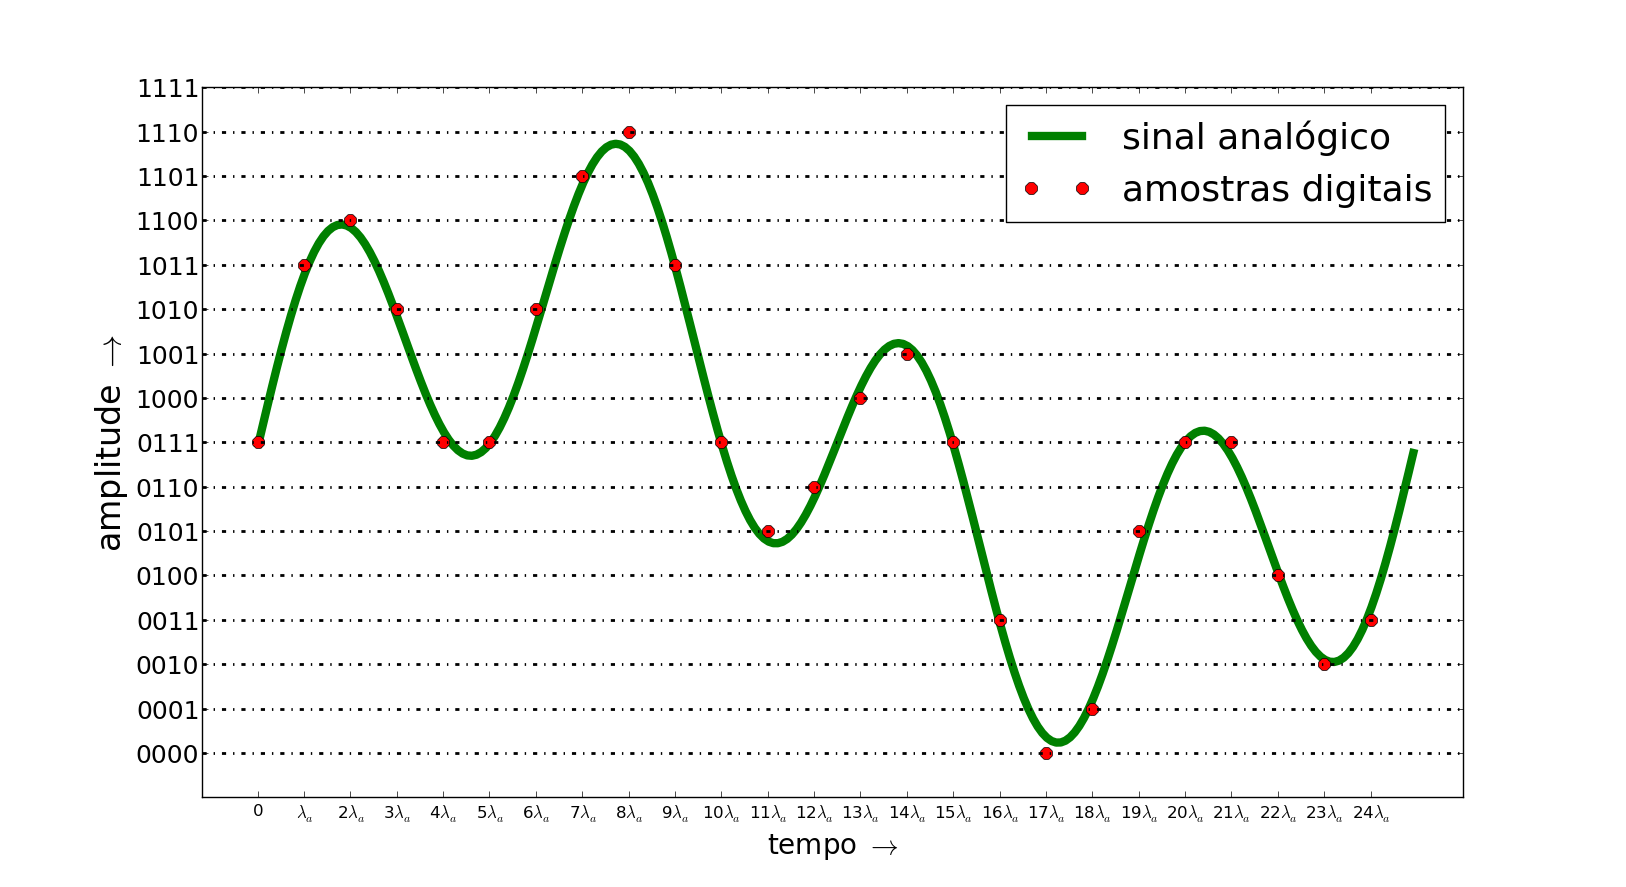
\includegraphics[width=\textwidth]{figuras/pcm}
        \label{fig:PCM}
\end{figure}

Nesta representação, é de conhecimento comum pelo teorema de Nyquist que não podemos representar frequências acima da metade da frequência de amostragem. Assim, se buscamos apreender as frequências audíveis, precisamos utilizar uma taxa de amostragem que seja ao menos o dobro da frequência mais alta capturada pelo sistema auditivo $f_a=2\times 20kHz=40kHz$. Este raciocínio está na base da utilização das frequências de amostragens $f_a=44.1kHz$ e $f_a=48kHz$, ambas utilizadas amplamente e são as taxas de amostragens padrão em \emph{Compact Disks} (CDs) e em sistemas de Rádio e TV, respectivamente~\cite{protocolosAudio}.

Do ponto de vista didático, é notável que praticamente todo processamento espectral sonoro seja praticável por somatórios quando tratamos do som discretizado. Estes mesmos procedimentos são efetuados por integrais quando estamos lidando com o som analógico, o que é consideravelmente mais complicado.




    \section{Arte sonora e teoria musical}

A música é comumente descrita como a arte manifesta pelos sons e silêncios. Embora esta definição esteja canonicamente correta, para as concepções usuais, ela está mais associada a uma ideia de arte sonora do que à música propriamente dita, pois para um ouvinte comum - e boa parte dos especialistas - uma 'música que seja música' pressupõe também a presença de uma métrica rítmica além de organizações de alturas que formem melodias e harmonias (veja sessão~\ref{notasMusica}). De qualquer forma, é importante reconhecer que a música do século XX ampliou esta concepção tradicional de música feita por notas que formam estruturas baseadas em ritmos, melodias e harmonias bem identificáveis. Isso ocorreu primeiramente na música de concerto, especialmente nas chamadas correntes eletrônica, concreta e eletroacústica. Já na década de 90 ficou claro que também a música popular, especialmente as músicas eletrônicas de dança, tinham por sua vez se desdobrado para abarcar não só os sons de altura definida e os organizações temporais bem estabelecidas dentro de métricas simples, mas também amálgamas sonoros ruidosos e disposições temporais fluídas e com sobreposições. Mesmo assim, a nota musical permanece paradigmática como 'unidade fundamental' das estruturas musicais. Além disso, as notas podem se desdobrar em sons que se desenvolvem no tempo, contemplando estes desenvolvimentos musicais recentes que foram supracitados (veja sessão~\ref{varInternas}).~\cite{Wisnick,Webern,Lerdahl,Cook}

A teoria musical é uma ampla área de estudos com várias abordagens divergentes e que engloba assuntos tão diversos quanto psicoacústica, convenções culturais de organização de alturas (e.g. uso de escalas) e formas musicais tradicionais, como a forma sonata e rondós, que consistem em estruturas paradigmáticas para uma música inteira~\cite{Zamacois,Schoenberg,microsound}. Neste trabalho, a abordagem deste assunto é bastante vinculada às aplicações dispostas no capítulo seguinte e estão apontadas no próprio texto mediante necessidade. Assim, não consideramos apropriado discorrer sobre estes assuntos aqui de forma independente, e para isso dispomos os títulos referenciados em nossa bibliografia. Recomendamos também o acompanhamento de um especialista, pois, na música, é comum um mesmo termo ser utilizado para designar diferentes conceitos e um mesmo conceito ser vinculado a diferentes termos, mesmo em contextos escolásticos.



    \section{Disponibilização computacional}
Os desenvolvimentos apresentados nesta dissertação incluem \emph{scripts} (i.e. pequenos programas) escritos em Python para disponibilização das tecnologias de forma explícita. Entendemos uma linguagem como o Python ou Scilab apropriada para esta tarefa
por ser de compreensão bastante simples, aproximando-se do que chamamos de pseudo-código~\cite{tutPython}. Outra faceta importante desta disponibilização é a utilização de um sistema de controle de versão para os textos, códigos e figuras. Assim, pode-se observar o desenvolvimento do trabalho e executar modificações sem tantas preocupações, pois todas elas ficam registradas individualmente e são reversíveis. Utilizamos para isso o sistema Git, tida como a segunda grande contribuição de Linus Torvals, sendo o próprio kernel Linux a primeira~\cite{gitBook}.

Os \emph{scripts} estão dispostos em duas versões: em Python puro~\cite{python}, i.e. sem bibliotecas externas, e em Python com Numpy e Audiolab~\cite{numpy,audiolab}. Esta segunda versão executa as rotinas através de chamadas à linguagem Fortran, muito eficiente em termos de processamento computacional e, consequentemente, em termos da duração necessária para a execução dos algoritmos.

Algum código já foi transcrito por terceiros para JavaScript com muita facilidade, o que torna estas contribuições potencialmente utilizáveis em navegadores bastante difundidos, como o Firefox e o Chromium.

Estas tecnologias são todas abertas, i.e. estão publicadas em licenças que permitem o uso, cópia, distribuição e utilização de quaisquer partes para geração de produtos derivados. Desta forma, os trabalhos aqui descritos estão disponíveis como parte de um repertório tecnológico livre que constitui um patrimônio da humanidade e é vinculado usualmente às comunidades de Software Livre e de Código Aberto\footnote{A comunidade e movimento chamada \emph{'Open Source'} é uma corrente que entende a publicação em licenças abertas de código computacional (e outras tecnologias) como sendo uma vantagem pragmática, possibilitando facilidades de desenvolvimento e vantagens de aprendizado e mercadológicas. A comunidade e movimento chamada \emph{'Free Software'} engloba este entendimento, mas adiciona a abordagem filosófica da liberdade e compartilhamento, e dá ênfase a isso. Ambas as correntes reforçam o entendimento de que o código computacional é o 'bem mais  precioso produzido atualmente' pois consiste em tecnologia condensada, reativa (pois executa, processa ou gera resultados), modular (pode ter partes copiadas e reutilizadas eficientemente) e replicada sem custo adicional (pois a cópia de texto tem custo baixíssimo). Muito frequentemente isso tudo está disposto em poucas linhas escritas.~\cite{Raymond,Lessig}}. Constatamos que, desta forma, ficam facilitadas as colaborações em processos de co-autoria e geração de materiais subsequentes.

    \section{Objetivos}
   \label{sec:objetivos}
Nosso objetivo principal nesta dissertação é dispor um sistema unificado que relacione elementos básicos da música às sequências amostrais do som digital. Este conhecimento já é existente ao menos em parte, tanto que diversos softwares comerciais apresentam desenvolvimentos relacionados~\cite{Steinberg, Waves, Sony}, mas não há uma apresentação unificada e concisa destas relações. Assim, a seguir apresentamos um texto coerente em que os elementos musicais são apresentados junto às sequências temporais envolvidas. Além disso, como parte da efetiva contribuição, entregamos implementações em código computacional (Python) destas relações e \emph{scripts} que resultam em pequenas peças musicais\footnote{Ou, de forma menos pretenciosa, montagens musicais, sequências musicais.}. 

Dada esta direção bem estabelecida, consideramos alguns objetivos secundários. Em primeiro lugar, a difusão de conhecimentos em programação e compreensão do código computacional é bastante potencializada através de práticas lúdicas, no caso a música. Outro objetivo considerado é a apresentação de um arcabouço de síntese sonora e musical com controle amostral, para o qual encontramos potenciais usos em experimentos psico-acústicos e síntese em alta definição (\emph{hi-fi}). Talvez por último, buscamos apresentar estes conteúdos de forma didática, quase um verdadeiro tutorial, possibilitando uma compreensão e uso facilitados, pois os assuntos tratados são de reconhecida complexidade: processamento de sinais, música, psico-acústica, para citar somente alguns exemplos. Deste ponto de vista didático, também reconhecemos importante a apresentação deste material na forma de hipertexto, em que cada \emph{script} e exemplo sonoro/musical seja acessível junto ao material teórico.
  
, deverá existir um arquivo tex com o nome introducao.tex no mesmo diretorio de tese.tex.

\afterpage{\blankpage}
\afterpage{\blankpage}
%% ------------------------------------------------------------------------- %%
\chapter{Introdução} %Nome do capítulo.
\label{cap:intro} 
\epigraph{"Tradicionalmente a notação musical é vista como um código através do qual sons, ideias musicais ou indicações para execução musical são registrados sob forma escrita."}{Edson S. Zampronha, \\ Notação, Representação e Composição, 2000}


O som pode ser definido como a propagação ondulatória e mecânica em um meio elástico
ou como a excitação dos mecanismos auditivos que resultam em sua percepção~\cite{Everest}. No primeiro
caso, estamos tratando de leis puramente físicas. No segundo caso, estamos lidando com um
fenômeno psicofísico. Nesta última abordagem encontramos lugar para a música, que escapa,
portanto, às leis fatídicas dos fenômenos naturais~\cite{Roederer}. A delicada tarefa de capturar estruturas
e artifícios musicais através das características do som discretizado
é exatamente a tarefa proposta por este trabalho. Para isso, entendemos cabível
abordar o som em sua representação digital e dispor os resultados em fórmulas matemáticas e implementações computacionais. 


    \section{Do som ao áudio digital}\label{sec:audio}

Em sua conceituação puramente física, o som é uma onda mecânica longitudinal de pressão e pode se propagar por qualquer meio material~\cite{}.
Embora o corpo humano possa captar sons cujas frequências estão fora da banda compreendida aproximadamente entre $20Hz$ e $20 kHz$, estas são as frequências chamadas audíveis e apreciadas pelo nosso aparelho auditivo.
 Considerada a velocidade do som no ar de $\approx 343.2\,m/s$ em condições usuais,
estes limites correspondem respectivamente aos comprimentos de onda $\frac{343.2}{20} = 17.16\,m$ e $\frac{343.2}{20000}=17.16\,mm$.

A efetiva audição humana destas vibrações consiste em um fenômeno complexo ainda sob intensa pesquisa, involvendo captações pelos ossos, estômago e orelha, além de funções de transferência da cabeça e dorso e processamento pelo sistema nervoso. Existe, no entanto, um órgão dedicado à tarefa de captura destas ondas, ao qual chamamos ouvido e cujo funcionamento decompõe o som em seu espectro senoidal antes de passar o estímulo para o sistema nervoso~\cite{Roederer}. Este papel central das componentes senoidais do som é crucial para os fenômenos musicais, o que pode ser notado tanto na composição de sons de interesse para a música, quanto nas afinações e escalas~\cite{floEsp}.

A representação do som é chamada áudio e usualmente usamos este termo para designar uma representação elétrica do som\footnote{Embora haja esta tendência e tradição de uso, os termos
som e áudio são, na verdade, usados de forma intercambiável~\cite{Everest}.}. O áudio pode ser proveniente da captura do som por microfones ou de síntese diretamente. O áudio digital consiste na sua representação sonora através de protocolos também digitais. Alguns destes protocolos são bastante elaborados, em geral visando resultar em quantidades reduzidas de dados para facilitar armazenamento e transferência dos arquivos~\cite{procFala}. Outras representações digitais do som são bastante diretas, consistindo em amostras igualmente espaçadas no tempo e cujas amplitudes individuais são registradas com um mesmo número de bits. Esta representação do som por amostras separadas por intervalos regulares $\lambda_a$ é a forma padrão de representação do som em tempo discreto e é chamada de modulação por código de pulsos e é denotada pela sigla PCM do inglês \emph{Pulse Code Modulation}.
Um som digital PCM é caracterizado pela frequência de amostragem $f_a=\frac{1}{\lambda_a}$ (também chamada de taxa de amostragem) e profundidade de bit, sendo este o número de bits utilizados para representar cada amostra~\cite{protocolosAudio}. Dispomos na figura~\ref{fig:PCM} um esquema gráfico de um áudio PCM. Observe que os $2^4=16$ grados disponíveis para a amplitude de cada amostra junto ao espaçamento regular $\lambda_a$ introduzem um erro de quantização. Estaremos apontando as formas de lidar com o ruído causado por estes erros de quantização sempre que pertinente.


\begin{figure}[h!]
    \centering
    \caption{Som digital em modulação por código de pulsos (PCM): 25 amostras representadas por 4 bits cada uma.}
        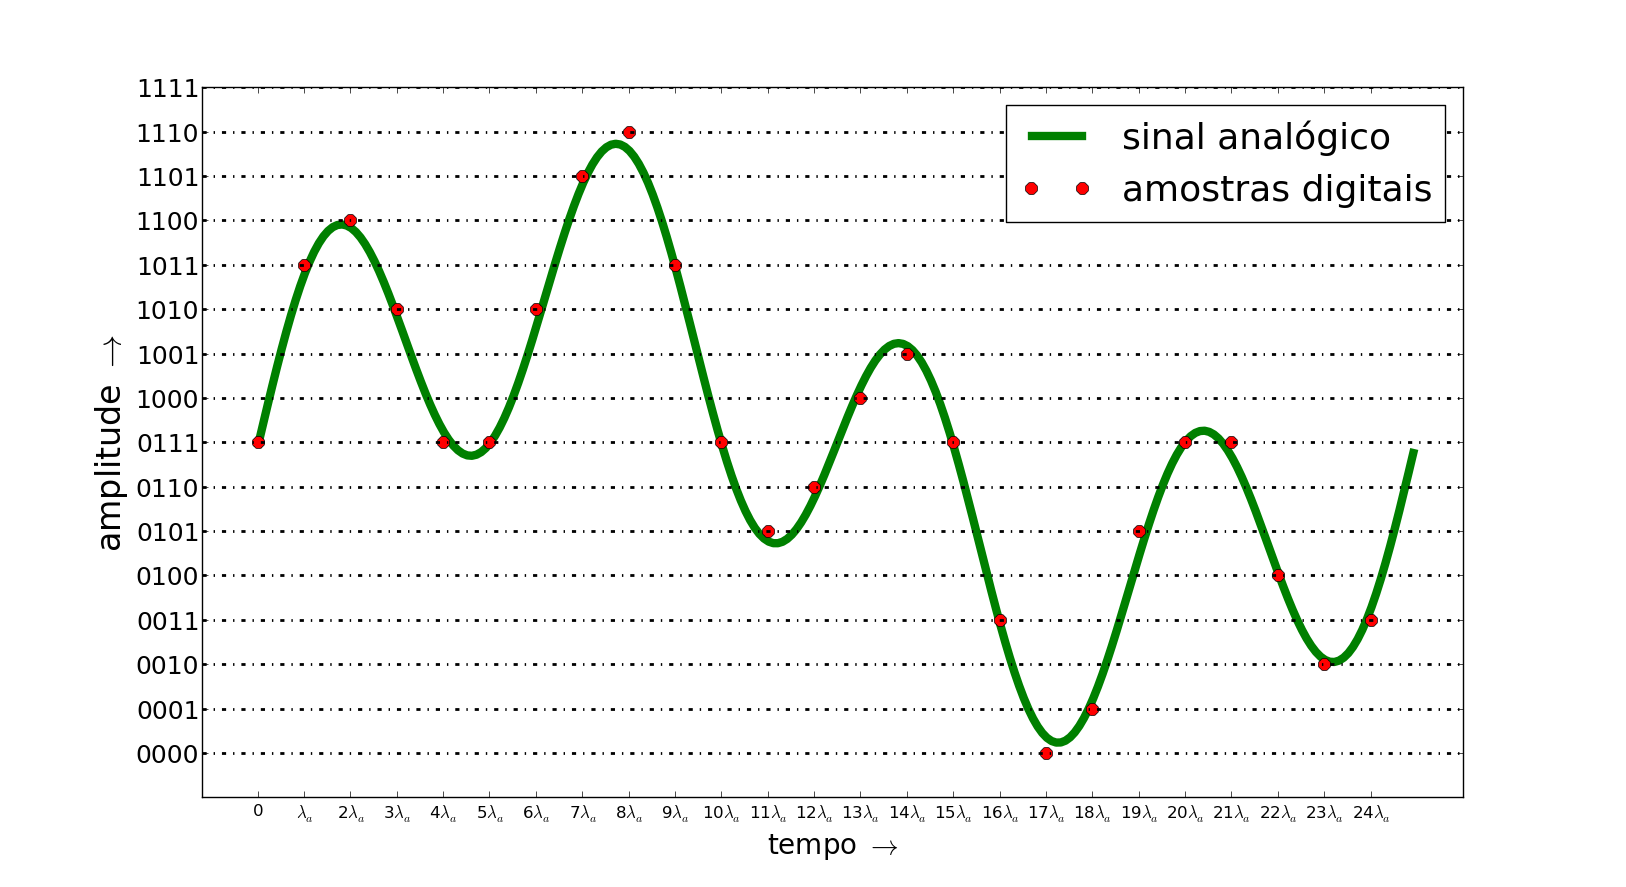
\includegraphics[width=\textwidth]{figuras/pcm}
        \label{fig:PCM}
\end{figure}

Nesta representação, é de conhecimento comum pelo teorema de Nyquist que não podemos representar frequências acima da metade da frequência de amostragem. Assim, se buscamos apreender as frequências audíveis, precisamos utilizar uma taxa de amostragem que seja ao menos o dobro da frequência mais alta capturada pelo sistema auditivo $f_a=2\times 20kHz=40kHz$. Este raciocínio está na base da utilização das frequências de amostragens $f_a=44.1kHz$ e $f_a=48kHz$, ambas utilizadas amplamente e são as taxas de amostragens padrão em \emph{Compact Disks} (CDs) e em sistemas de Rádio e TV, respectivamente~\cite{protocolosAudio}.

Do ponto de vista didático, é notável que praticamente todo processamento espectral sonoro seja praticável por somatórios quando tratamos do som discretizado. Estes mesmos procedimentos são efetuados por integrais quando estamos lidando com o som analógico, o que é consideravelmente mais complicado.




    \section{Arte sonora e teoria musical}

A música é comumente descrita como a arte manifesta pelos sons e silêncios. Embora esta definição esteja canonicamente correta, para as concepções usuais, ela está mais associada a uma ideia de arte sonora do que à música propriamente dita, pois para um ouvinte comum - e boa parte dos especialistas - uma 'música que seja música' pressupõe também a presença de uma métrica rítmica além de organizações de alturas que formem melodias e harmonias (veja sessão~\ref{notasMusica}). De qualquer forma, é importante reconhecer que a música do século XX ampliou esta concepção tradicional de música feita por notas que formam estruturas baseadas em ritmos, melodias e harmonias bem identificáveis. Isso ocorreu primeiramente na música de concerto, especialmente nas chamadas correntes eletrônica, concreta e eletroacústica. Já na década de 90 ficou claro que também a música popular, especialmente as músicas eletrônicas de dança, tinham por sua vez se desdobrado para abarcar não só os sons de altura definida e os organizações temporais bem estabelecidas dentro de métricas simples, mas também amálgamas sonoros ruidosos e disposições temporais fluídas e com sobreposições. Mesmo assim, a nota musical permanece paradigmática como 'unidade fundamental' das estruturas musicais. Além disso, as notas podem se desdobrar em sons que se desenvolvem no tempo, contemplando estes desenvolvimentos musicais recentes que foram supracitados (veja sessão~\ref{varInternas}).~\cite{Wisnick,Webern,Lerdahl,Cook}

A teoria musical é uma ampla área de estudos com várias abordagens divergentes e que engloba assuntos tão diversos quanto psicoacústica, convenções culturais de organização de alturas (e.g. uso de escalas) e formas musicais tradicionais, como a forma sonata e rondós, que consistem em estruturas paradigmáticas para uma música inteira~\cite{Zamacois,Schoenberg,microsound}. Neste trabalho, a abordagem deste assunto é bastante vinculada às aplicações dispostas no capítulo seguinte e estão apontadas no próprio texto mediante necessidade. Assim, não consideramos apropriado discorrer sobre estes assuntos aqui de forma independente, e para isso dispomos os títulos referenciados em nossa bibliografia. Recomendamos também o acompanhamento de um especialista, pois, na música, é comum um mesmo termo ser utilizado para designar diferentes conceitos e um mesmo conceito ser vinculado a diferentes termos, mesmo em contextos escolásticos.



    \section{Disponibilização computacional}
Os desenvolvimentos apresentados nesta dissertação incluem \emph{scripts} (i.e. pequenos programas) escritos em Python para disponibilização das tecnologias de forma explícita. Entendemos uma linguagem como o Python ou Scilab apropriada para esta tarefa
por ser de compreensão bastante simples, aproximando-se do que chamamos de pseudo-código~\cite{tutPython}. Outra faceta importante desta disponibilização é a utilização de um sistema de controle de versão para os textos, códigos e figuras. Assim, pode-se observar o desenvolvimento do trabalho e executar modificações sem tantas preocupações, pois todas elas ficam registradas individualmente e são reversíveis. Utilizamos para isso o sistema Git, tida como a segunda grande contribuição de Linus Torvals, sendo o próprio kernel Linux a primeira~\cite{gitBook}.

Os \emph{scripts} estão dispostos em duas versões: em Python puro~\cite{python}, i.e. sem bibliotecas externas, e em Python com Numpy e Audiolab~\cite{numpy,audiolab}. Esta segunda versão executa as rotinas através de chamadas à linguagem Fortran, muito eficiente em termos de processamento computacional e, consequentemente, em termos da duração necessária para a execução dos algoritmos.

Algum código já foi transcrito por terceiros para JavaScript com muita facilidade, o que torna estas contribuições potencialmente utilizáveis em navegadores bastante difundidos, como o Firefox e o Chromium.

Estas tecnologias são todas abertas, i.e. estão publicadas em licenças que permitem o uso, cópia, distribuição e utilização de quaisquer partes para geração de produtos derivados. Desta forma, os trabalhos aqui descritos estão disponíveis como parte de um repertório tecnológico livre que constitui um patrimônio da humanidade e é vinculado usualmente às comunidades de Software Livre e de Código Aberto\footnote{A comunidade e movimento chamada \emph{'Open Source'} é uma corrente que entende a publicação em licenças abertas de código computacional (e outras tecnologias) como sendo uma vantagem pragmática, possibilitando facilidades de desenvolvimento e vantagens de aprendizado e mercadológicas. A comunidade e movimento chamada \emph{'Free Software'} engloba este entendimento, mas adiciona a abordagem filosófica da liberdade e compartilhamento, e dá ênfase a isso. Ambas as correntes reforçam o entendimento de que o código computacional é o 'bem mais  precioso produzido atualmente' pois consiste em tecnologia condensada, reativa (pois executa, processa ou gera resultados), modular (pode ter partes copiadas e reutilizadas eficientemente) e replicada sem custo adicional (pois a cópia de texto tem custo baixíssimo). Muito frequentemente isso tudo está disposto em poucas linhas escritas.~\cite{Raymond,Lessig}}. Constatamos que, desta forma, ficam facilitadas as colaborações em processos de co-autoria e geração de materiais subsequentes.

    \section{Objetivos}
   \label{sec:objetivos}
Nosso objetivo principal nesta dissertação é dispor um sistema unificado que relacione elementos básicos da música às sequências amostrais do som digital. Este conhecimento já é existente ao menos em parte, tanto que diversos softwares comerciais apresentam desenvolvimentos relacionados~\cite{Steinberg, Waves, Sony}, mas não há uma apresentação unificada e concisa destas relações. Assim, a seguir apresentamos um texto coerente em que os elementos musicais são apresentados junto às sequências temporais envolvidas. Além disso, como parte da efetiva contribuição, entregamos implementações em código computacional (Python) destas relações e \emph{scripts} que resultam em pequenas peças musicais\footnote{Ou, de forma menos pretenciosa, montagens musicais, sequências musicais.}. 

Dada esta direção bem estabelecida, consideramos alguns objetivos secundários. Em primeiro lugar, a difusão de conhecimentos em programação e compreensão do código computacional é bastante potencializada através de práticas lúdicas, no caso a música. Outro objetivo considerado é a apresentação de um arcabouço de síntese sonora e musical com controle amostral, para o qual encontramos potenciais usos em experimentos psico-acústicos e síntese em alta definição (\emph{hi-fi}). Talvez por último, buscamos apresentar estes conteúdos de forma didática, quase um verdadeiro tutorial, possibilitando uma compreensão e uso facilitados, pois os assuntos tratados são de reconhecida complexidade: processamento de sinais, música, psico-acústica, para citar somente alguns exemplos. Deste ponto de vista didático, também reconhecemos importante a apresentação deste material na forma de hipertexto, em que cada \emph{script} e exemplo sonoro/musical seja acessível junto ao material teórico.
  

\afterpage{\blankpage}
%%% ------------------------------------------------------------------------- %%
\chapter{Fundamentos teóricos e técnicos} %Nome do capítulo.
% \label{cap:intro} %Rótulo para futura referência ao capítulo. Em qualquer lugar da tese, você poderá citar este capítulo através de ~\ref{cap:introducao}. Você escolhe o argumento de \label e pode ser qualquer coisa (Ex: \label{Procedimento_Experimental})

\section{Áudio}

  \subsection{O som e a audição}

O som é o fenômeno físico de propagação de ondas mecânicas. Ele pode
somente ocorrer na presença de matéria, como ar, água, ferro ou madeira.
São ondas de pressão que se deslocam com velocidade caracterizada principalmente
pelo meio material e também pelas condições como a temperatura e a pressão.
O vácuo é um isolante acústico perfeito.

Tipicamente a velocidade do som é de $~340 m/s $ e é
relativamente estável\footnote{$343.2 m/s$ em ar seco a 20 °C (68 °F)}.
As modificações de sonoridades com o clima é devido a alterações
dos materiais que os geram e acústica do ambiente, não devido a alterações
desta velocidade de propagação do som no meio atmosférico.

Falar de fonons e coisas assim? Quais aspectos do som devemos cobrir?

      \subsubsection{A audição e a psicofísica}

A audição é definida com a percepção de vibrações mecânicas com
ou sem a contribuição direta do tato. Em diversos
seres vivos, encontramos um órgão dedicado a captar e transmitir
estas vibrações mecânicas (som) para o sistema nervoso.

O ouvido humano cumpre exatamente este papel. Um esquema básico
do ouvido humano conta com 3 divisões. No ouvido externo está a orelha.
No médio, os martelinhos e o tímpano. No ouvido interno tem a cóclea
e os cíclios. Uma visualização simplificada do ouvido humano está abaixo.


FIGURA MOSTRANDO ENTRADA DE VIBRAÇÃO E TRANSMISSÃO AO CÉREBRO

Vale notar que a audição conta em grande parte com o tato e potencialmente
outros órgãos, como o estômago.

Já a psicofísica busca relacionar características físicas do fenômeno sonoro
com as percepções individuais resultantes\footnote{PsycoPy para escrever experimentos psicofísicos em Python: http://www.psychopy.org/}.
Importantes exemplos destas relações
são a escala logarítimica que a percepção linear das alturas assume no
domínio da frequência e as curvas iso-audíveis (conhecidas como curvas de Fletcher-Münsen).
EXPLICAR MELHOR?

Outro importante aspecto da psicofísica do som - e da música - é a resolução da percepção
e a capacidade de notar características do espectro em contextos específicos. O mascaramento
de frequências é a base na qual se faz compactadores de tamanhos de arquivos de áudio. Sabe-se
que, por exemplo, no extremo grave, não conseguimos distinguir duas senóides a quase um tom de
diferença. Alguns outros importantes fenômenos psicoacústicos estudados com fins tecnológicos, científicos e artísticos são: espacialidade,
relação da percepção de volume com espectro agudo e reverberação e compreensibilidade de sinais de fala.


\subsection{Áudio digitalizado}
Enquanto estamos interessados na variação de pressão do ar, podemos de fato utilizar
um microfone para converter esta variação de pressão em sinal elétrico (usualmente voltagem).
Convertemos assim o som (fenômeno físico) em áudio (sinal elétrico relacionado).
Neste processo, o sinal é amostrado no tempo geralmente através do uso de
um conversor A/D\footnote{Conversor Analógico para Digital. Para as aplicações descritas aqui é tipicamente uma placa som.}. Assim, um evento sônico
torna-se um sinal digital, usufruindo das facilidades para armazenamento, transmissão e
processamento da nossa tecnologia digital atual.

Esta amostragem do sinal de áudio é bastante elaborada e dependente de manejo de hardware. Para
aprofundar este tema, recomendamos [][][] e uma representacao esquematica deste processo
se encontra na figura.	 
% \figure{fig:AD}.

FIGURA MOSTRANDO UMA ONDA ANALOGICA E ELA REPRESENTADA POR PONTOS.

A representação digital do som pode ser feita de diversas formas.
A representação PCM (Pulse Code Modulation) canônica possui amostras
igualmente espaçadas no tempo e para cada uma utiliza precisão com o mesmo
número de bytes.

[Figura com onda amostrada com limites superior inferior e valores das amostras]

Note que o áudio digital possue também uma velocidade no espaço de amostragem.
Quantidades como $8kHz$, $44.1kHz$, $48kHz$
descrevem quantidade de amostras em cada segundo com que o áudio examinado foi feito ou
está sendo utilizado.

O importante Teorema de Nyquist demonstra que em um sinal digital só se consegue representar
frequências até metade da taxa de amostragem. Ou seja, em um áudio com $48kHz$ de taxa de amostragem,
conseguimos representar frequências de até $24kHz$. A frequência de Nyquist é exatamente a metade
da frequência de amostragem e é a frequência mais aguda que aquele sinal pode representar.
(PROVA ELEGANTE DO TEOREMA DE Nyquist? TAMB REFERENCIAR OS SCRIPTS PARA ESTUDO DO FENOMENO)

Além da representação PCM, pode-se utilizar outros formatos para o armazenamento do áudio. Alguns
destes formatos apresentam perda de qualidade e são mais indicados para serem transmitidos via rede ou
para armazenamento\footnote{Os formatos que apresentam perda de qualidade com relação
ao PCM são chamados formatos \emph{lossy}, os que não apresentam perda de qualidade
são chamados \emph{loseless}}. Abaixo está uma tabela com alguns dos formatos mais importantes que possuímos:

TABELA DE FORMATOS


\subsection{Processamento de áudio}

Síntese, alteração ou análise.

\begin{itemize}
    \item Geral
    \item Voz
    \item Música
\end{itemize}

Procedimentos básicos: Lookuptable, sample. Processamento
espectral. Outros processamentos.

Vincular a um apêndice com excertos de código.

\section{Disponibilização da tecnologia em código}

  \subsection{Python}


  \subsection{Git}


%% ------------------------------------------------------------------------- %%
\chapter{Desenvolvimentos e resultados} %Nome do capítulo.
\label{cap:resultados} %Rótulo para futura referência ao capítulo. Em qualquer lugar da tese, você poderá citar este capítulo através de ~\ref{cap:introducao}. Você escolhe o argumento de \label e pode ser qualquer coisa (Ex: \label{Procedimento_Experimental})
Os resultados explicitados nesta dissertação estão focados no processamento de 
áudio através de códigos em liguagens de programação de computadores e
voltado para a música e na síntese de estruturas musicais. O tema é amplo
e pertinente o suficiente para contar atualmente com ampla bibliografia e um histórico
que remonta desde a própria história da computação e das linguagens de programação.
Desta forma, entendemos cabível focar este texto nas empreitadas realizadas pelos autores
da presente dissertação, com foco nas realizações do primeiro autor. São usos
reais destas tecnologias, manifestadas de forma cultural e com repercussões
sociais, como poderá é relatado neste mesmo capítulo.

Tais realizações possuem um espectro amplo
dentro do escopo proposto e constitui um percurso relativamente completo
pelas possibilidades e decorrências da abordagem da música pelo código computacional\footnote{ao menos dentro do se denomina 'Cultura Livre', veja o primeiro capítulo do presente escrito para maiores informações}.

Estaremos abordando experimentos abertos em áudio, abordagens musicais pelo código, incluindo música em tempo real, diferido, na matéria e repercussões no tecido social. De forma a relatar os resultados destas investidas, segue uma sessão sobre ações coletivas realizadas através das mobilizações que estes códigos criaram, e as estruturas virtuais mantidas na intenet relacionadas a estas mobilizações e ações. Por fim, alguns materiais didáticos criados pelo autor - que possuem algum papel emblemático - são também expostos por comporem o arsenal de repercussões desta investida no em som e código. 

  \section{Experimentos abertos em áudio: LADSPAs, Wavelets e Redes Complexas}

Todos os desenvolvimentos desta dissertação estão em repositórios abertos\cite{repositorios-tese-dev}.
Alguns foram especialmente importantes como percurso para o que é apresentado neste
escrito. Ou seja, são explorações que manifestaram diferentes aspectos
do trabalho do código voltado para o áudio e a música.

O código para a arte sonora, incluindo a musical, manifesta-se como cultura pois é fruto de práticas
espontâneas, diárias e coletivas.
\footnote{As chamadas culturas biopunk, ciberpunk, cipherpunk, hacker, digital e outras mais,
possibilitadas aos recentes desenvolvimentos em telecomunicação, dizem respeito em menor
ou maior grau à produção de código como cultura.}

A seguir apresentamos alguns bons exemplos dos desenvolvimentos
desta dissertação especificamente em áudio, sem o envolvimento direto da música. São
códigos de necessidade para música, mas de uso mais geral e cuja implementação
requer muito mais de processamento de sinais e computação do que de música propriamente dito.

      \subsubsection{Plugins LADSPA e lv2}
      [repos AE, LM, wiki EL, historico CDTL]
LADSPA (Linux Audio Developers Simple Plugin API) é a API livre\footnote{Veja o Capítulo 1 para a definição de livre neste contexto.} estabelecida de plugins de áudio até a presente data. A última versão liberada desta API é a 1.1, em uso corrente até hoje e é de 2002 segundo os arquivos de cabeçalho relacionados.

A exploração de APIs específicas foge ao escopo do presente texto e os códigos completos podem ser encontrados pela rede, junto a tutoriais e plugins de exemplo. O código destes desenvolvimentos e pertinente ao áudio são relativos à síntese e remoção de ruídos. Da síntese, exitem abordagens mais puristas, que no caso sintetiza ruído branco e filtra para resultar nos espectros desejados (veja logo abaixo para maiores especificações). Uma abordagem menos purista porém mais eficiente é a de usar uma amostra curta do ruído e reproduzí-la indefinidamente através de \emph{cross-fades}.

Já na remoção de ruídos as abordagens são as mais variadas e extremamente dependentes da aplicação. A complexidade dos algorítmos pode atingir níveis de especialidade em processamento de sinais que merecem um trabalho dedicado. Aqui iremos expor somente sobre remoção de ruído \emph{'Hum'} causado usualmente pela corrente alternada que alimenta os equipamentos utilizados.

Abaixo dispomos explicações breves sobre os diferentes ruídos e os códigos relacionados. Preferimos expor em Python os códigos de síntese
por questão de clareza e coerência com o resto do texto\footnote{Os códigos em C/C++ e a implementação como plugin lv2 está no repositório git LV2 como pode ser visto em: http://labmacambira.git.sourceforge.net/git/gitweb-index.cgi}.

O procedimento de reprodução do ruído através de uma amostra repetida e em crossfade é a seguinte:

[código da reprodução do ruído em loop e croos-fade ~10 linhas]

Sintetizando diferentes ruídos\footnote{Dado o propósito do texto e da implementação, utilizamos nomenclaturas utilizadas na música para os ruídos, como se pode notar.}:
\begin{itemize}
    \item Ruído Branco: 
    \item Ruído Rosa:
    \item Ruído Marrom:
    \item Ruído Violeta:
    \item Ruído Azul:
    \item Ruído Violeta:
    \item Ruído Cinza:
    (nao oficiais)
    \item Ruído Vermelho:
    \item Ruído Laranja:
    \item Ruído Preto:
    \item Ruído Branco Ruidoso:
    \item Ruído Preto Ruidoso:
    \item Clicks:
\end{itemize} 

A remoção de ruído Hum é baseada em uma sequência de filtros notch (ver fundamentos) idealmente dispostos nos harmônicos da frequência de oscilação da corrente elétrica. Cada um destes filtros deve permitir ajustes finos no fator de qualidade e também na frequência central pois trata-se de um sistema real passivel dos mais diversos efeitos de distorção do modelo ideal. Abaixo expomos o código em Python para tal \emph{removedor de ruído} como é chamado. O código C/C++ e a implementação como plugin está no mesmo repositório disponibilizado para a síntese de ruídos.

[código e explicação do remodedor de ruído Hum]


      \subsubsection{Protocolo de compactação de áudio via wavelets, polinômios e permutações}
Criado por Rafael Santos Mendes em conjunto com o primeiro autor deste trabalho e em decorrência do mestrado de André Luvizotto, este método
consiste em aproximar cada folha de uma decomposição WaveletPacket por um polinômio e uma permutação. A permutação facilita a aproximação polinomial, pois leva folhas WP de coeficientes ordenados para sucessões melhor comportadas de seus valores\footnote{O método é descrito em um artigo de 2009: Compressão de Áudio via Wavelets, Aproximações Polinomiais e Permutações [Fabbri, Mendes]}.
Representamos cada permutação por um conjunto ordenado de números inteiros. Já o polinômimo possui poucos coeficientes (usualmente 6 ou 8) e os representamos como um conjunto ordenado de variáveis de tipo ponto flutuante.


      \subsubsection{Processamento de voz via redes complexas}
Conversar com Chu e com Luciano e decidir se retiro esta sessão ou mantenho.

      [codigos bem comentados no audio experiments. Apresentação do trabalho "Speech Polarity Detection using Complex Networks Measures: First Explorations no Complenet de 2010"]



\section{Música no Som Digitalizado}

%\subsection{Caracterização da nota musical discretizada}
\subsection{Caracterização da nota musical digital}
%\subsection{Caracterização da nota musical digital}
A música é tradicionalmente pensada através de unidades chamadas notas. Em sua concepção
simples, as notas possuem ao menos duração, volume, altura e timbre. Embora estas
sejam características psicofísicas, podemos lidar com elas através de suas características
fisicamente mensuráveis.
Em primeiro lugar, estamos tratando diretamente da representação digital do som. Isso em uma
sequência de amostras igualmente espaçadas no tempo. Desta forma, definimos a
frequência (ou taxa) de amostragem $f_a$ como o número de amostras por segundo do áudio digital e
a sequência $T_i=\{t_i\}$ como um conjunto ordenado de amostras reais separadas por $\delta_a=1/f_a$ segundos.


\subsubsection{Duração}
Desta forma, visando uma nota musical de duração $\Delta$,
teremos uma sequência de $ \Delta . f_a $ amostras\footnote{Observe o abuso de notação:
o limite superior de uma sequência é um número natural, mas $ \Delta . f_a $
só satisfaz esta condição em casos muito excepcionais. Procederemos assim por simplicidade. 
Explicitaremos em texto quando for crucial o procedimento relativo à parte fracionária dos índices
ou de seus limites.}:

\begin{equation}
T_{i}^{\Delta}={\{t_i\}}_{i=0}^{\Delta . f_a - 1}
\end{equation}


\subsubsection{Volume}
O volume depende da reverberação e distribuição dos harmônicos - dentre outras medidas psicofísicas~\cite{chowningVolume} - mas num primeiro momento podemos lidar com ele de forma prática e geral através da potência da onda:

\begin{equation}\label{potencia}
pot(T_i^{\Delta})=\frac{\sum_{i=0}^{\Delta . f_a -1} t_i^2}{\Delta . f_a}
\end{equation} 

Como o volume final dependerá da amplificação do sinal nos falantes, o mais importante é a potência relativa de uma nota em relação às outras ou de um trecho da música em relação ao resto. As diferenças de volume são medidas em decibeis, que são
calculadas diretamente com as amplitudes, energias ou potências\footnote{Lembrando que, devido à nossa percepção logarítmica,
em um som de volume $v$ a redução da potência $p$ para uma mesma fração $\nu . p $ 
com $\nu \in [0,1]$ é sentido como a mesma diminuição do volume $v-\kappa$ com $\kappa \geq 0$.}:

\begin{equation}\label{decibeis}
V_{dB}=10log_{10}\frac{pot(T^{'}_i)}{pot(T_i)}
\end{equation}

A quantidade adimensional é denotada pela unidade decibeis ($dB$). A cada 10 $dB$s atribuímos canonicamente
a sensação de "volume dobrado". Importantes resultados de referência são os equivalente em $dB$s de se dobrar
a amplitude ou a potência:

\begin{equation*}
se \quad  t_i^{'}=2 . t_i \quad \Rightarrow \quad pot(T^{'}_i)=4 . pot(T_i) \quad \Rightarrow \quad V^{'}_{dB}=10log_{10} 4 \quad  \approx \quad 6 dB
\end{equation*}
\begin{equation*}
se \quad pot(T^{'}_i)=2 pot(T_i) \quad \Rightarrow \quad V^{'}_{dB}=10log_{10} 2 \quad \approx \quad 3 dB
\end{equation*}

Outro valor de referência é a amplificação necessária para que uma sequência tenha o volume dobrado ($10dB$s a mais):

\begin{gather}
10log_{10}\frac{pot(T^{'}_i)}{pot(T_i)} = 10 \quad \Rightarrow \quad \sum_{i=0}^{\Delta.f_a-1}t^{'2}_i=10\sum_{i=0}^{\Delta.f_a-1}t_i^2=\sum_{i=0}^{\Delta.f_a-1}(\sqrt{10}.t_i)^2 \\
\therefore \quad t^{'}_i=\sqrt{10}t_i \quad \Rightarrow \quad t^{'}_i \approx 3,16t_i
\end{gather}

Ou seja, é necessário pouco mais que triplicar a amplitude para que tenhamos volume drobrado.

Estes valores servem de guia para os aumentos e diminuições dos valores absolutos que compõem as
sequências de amostras sonoras que visam atingir efeitos musicais. A conversão direta de decibeis
em amplitude se dá da seguinte forma:

\begin{equation}\label{ampDec}
A = 10^{\frac{V_{dB}}{20}}
\end{equation}

Onde $A$ é o fator multiplicativo entre as médias dos valores absolutos das amplitudes dos sinais comparados.

Neste ponto, correspondendo a uma partícula musical (uma nota), estabelecemos uma sequência cuja
duração e intensidade conseguimos controlar\footnote{Basta alterarmos o tamanho da sequência para alterarmos
a duração ou multiplicarmos as os elementos da sequência por algum valor normalizador}. 

\subsubsection{Altura\footnote{Com ganho de simplicidade e sem perda de generalidade, considere o índice $i=a/b$ como o inteiro mais próximo da divisão $a/b$.}}

A altura é especificada pela frequência fundamental. A frequência fundamental $f_0$ especifica uma periodicidade temporal
com ciclo de duração $\delta_{f_0} = 1/f_0$. Esta duração multiplicada pela taxa de amostragem $f_a$ resulta no número de amostras
do ciclo $\lambda_{f_0}=f_a . \delta_{f_0} =f_a/f_0$. Evidente que, sendo $T_i^f$ a sequência sonora de frequência fundamental $f$:
    
\begin{equation}\label{periodicidade}
     T^f_i=\{ t_i^f \}=\{ t^f_{i+\lambda_{f}}  \}= \{ t^f_{i+\frac{f_a}{f}} \}
\end{equation}

\subsubsection{Timbre}
Enquanto o período da onda corresponde a uma frequência fundamental, o percurso
da onda sonora dentro do período define um espectro harmônico e portanto
um timbre\footnote{O timbre é uma característica subjetiva e complexa. Fisicamente,
o timbre é multidimensional e dado pelo comportamento temporalmente dinâmico
de energias em componentes espectrais tanto harmônicas quanto ruidosas.  Vale salientar que nem tudo
o que se atribui ao timbre se acha manifesto em diferenças espectrais. Uma mesma nota
possui diferentes matizes espectrais, um mesmo instrumento possui diferentes timbres. Mesmo
assim se fala que uma nota e um instrumento possuem um timbre. Por último, até
aspectos culturais ou circunstanciais alteram nossa percepção timbrística.
Na música, espectros
sonoros com diferenças mínimas resultam em
 timbres com diferenças expressivamente cruciais.
}.

O caso mais simples (e mais importante, como veremos adiante) é o do espectro que consiste somente
de sua própria fundamental $f$. Este é o caso da senóide, frequência em movimento oscilatório puro chamado
movimento harmônico simples. Seja $S_i^f$ uma sequência cujas amostras
$s_i^f$ descrevem uma senóide de frequência $f$:

\begin{equation}\label{senoide}
     S^f_i=\{ s^f_i \}=\Bigl\{ \sin\bigl(2\pi \frac{i}{\lambda_f} \bigr)  \Bigr\} = \Bigl\{ \sin\bigl(2\pi f \frac{i}{f_a}\bigr)  \Bigr\} 
\end{equation}

Onde $\lambda_f=\frac{f_a}{f}=\frac{\delta_f}{\delta_a} \;$ é o número de amostras do período\footnote{Neste ponto já se tem toda a base para música "reduced-fi", ver APÊNDICE ~\ref{APENDICE XX}}.

De forma semelhante, outras formas de onda são utilizadas na música por suas qualidades
espectrais e simplicidade. Enquanto a senóide é um ponto isolado no espectro, estas formas
de onda apresentam cadeias de componentes harmônicos e usos específicos.
As formas de onda especificadas em ~\ref{denteDeSerra}, ~\ref{triangular} e ~\ref{quadrada} são dispostas graficamente na figura ~\ref{fig:formasDeOnda}. 
São as formas de onda artificiais tradicionalmente usadas na música para síntese e controle oscilatório de variáveis, apresentam diversos usos também fora da música.

A dente de serra apresenta todos os componentes da série
harmônica com energia decrescente de $-6dB/oitava$. A sequência de amostras temporais pode ser descrita da seguinte forma:
\begin{equation}\label{denteDeSerra}
     D^f_i=\{ d^f_i \}=\Bigl\{ 2\frac{i\,\%\lambda_f}{\lambda_f} -1 \Bigr\}
\end{equation}

A forma de onda triangular apresenta somente os harmônicos ímpares caindo a $-12dB/oitava$:
\begin{equation}\label{triangular}
     T^f_i=\{ t^f_i \}=\Bigl\{1- \Bigl| 2 - 4\frac{i\,\%\lambda_f}{\lambda_f} \Bigr| \Bigr\}
\end{equation}

A onda quadrada apresenta somente os harmônicos ímpares caindo a $-6dB/oitava$:
\begin{equation}\label{quadrada}
     Q^f_i=\{ q^f_i \}= \left\{
         \begin{array}{l l}
              1 & \quad \text{para} \; \; (i\,\%\lambda_f)   <  \lambda_f /2  \\
              -1 & \quad \text{caso contrário}\\
         \end{array} \right.
\end{equation}

A dente de serra é um ponto de partida comum para a síntese subtrativa pois possui
ambos os harmônicos pares e ímpares e em grande quantidade (alguma filtragem atenuante
é útil nos médios e agudos para que o som ganhe naturalidade e fique mais agradável).
Por este mesmo motivo, os harmônicos atenuados da onda triangular
a faz a mais funcional - dentre as citadas - para ser usada sem nenhum tratamento.

Para citar também um uso possível da onda quadrada, ela pode ser usada em uma síntese
subtrativa que vise imitar um clarinete. Este instrumento também só apresenta os
componentes ímpares do espectro harmônico e a onda quadrada pode convir com sua energia abundante nas altas frequências.



\begin{figure}[h!]
    \centering
    \caption{Formas de onda musicais básicas}
        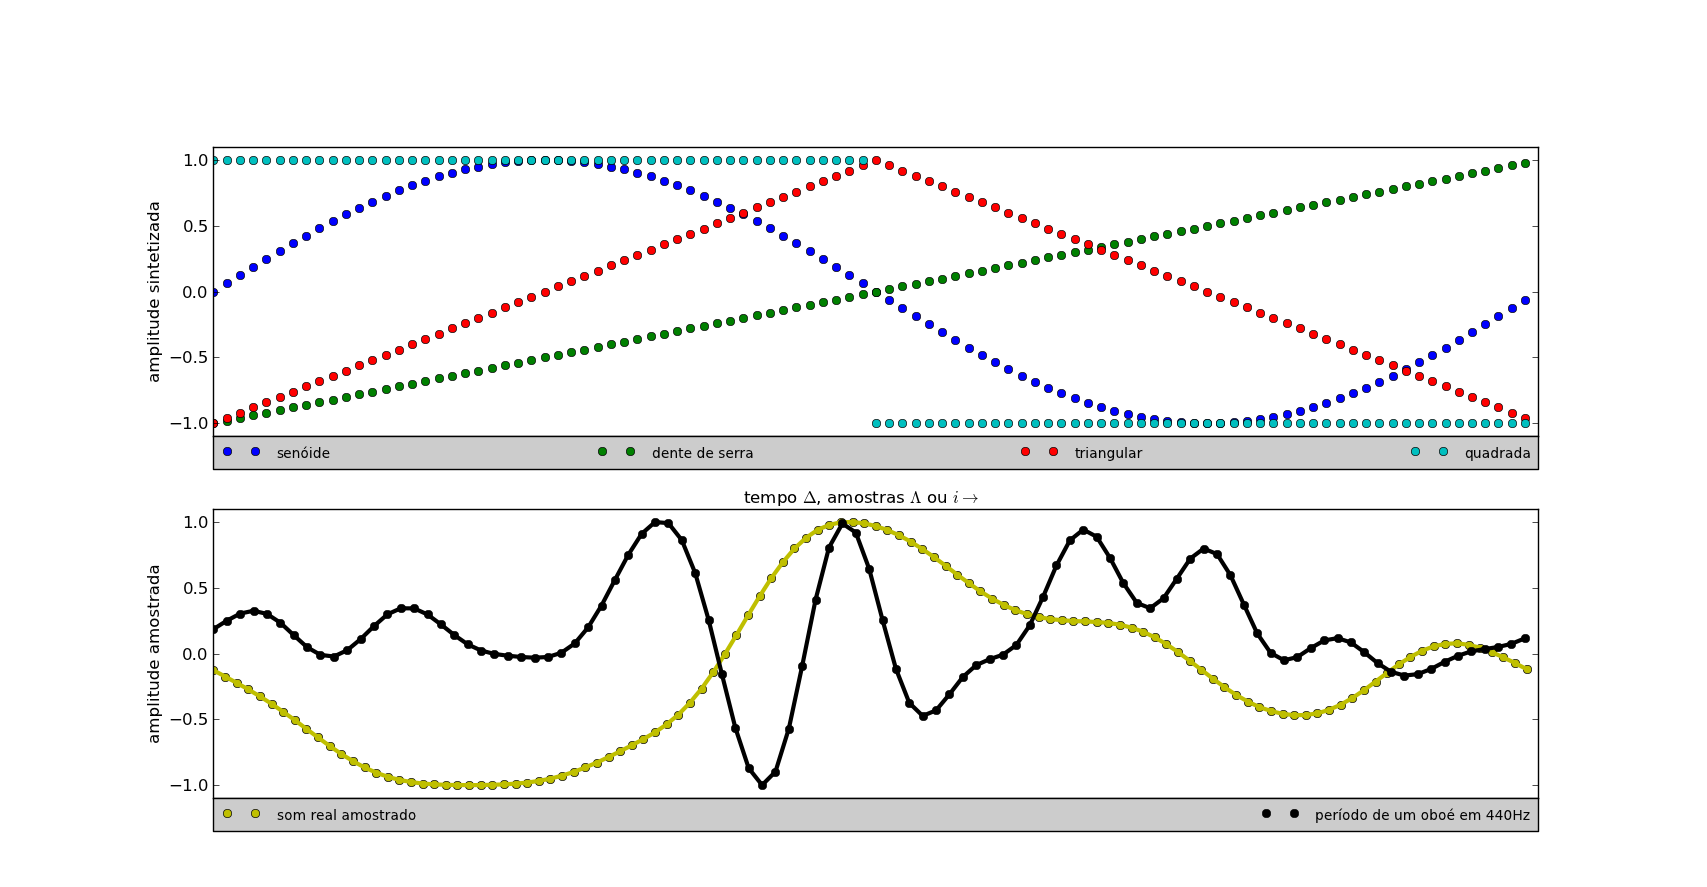
\includegraphics[width=\textwidth]{figuras/formasDeOnda5}
        \label{fig:formasDeOnda}
\end{figure}



A figura ~\ref{fig:formasDeOnda} apresenta
as formas de onda descritas nas equações ~\ref{senoide}, ~\ref{denteDeSerra}, ~\ref{triangular} e ~\ref{quadrada} para $\lambda_f=100$ (período
de $100$ amostras).
Se $t_a=44,1 kHz$, como em padrões PCM e de Compact Disks, a onda possui frequência fundamental $f=\frac{f_a}{\lambda_f}=\frac{44100}{100} = 441 \; Herz $. Um lá\footnote{Um lá 4, logo acima do dó central, no segundo espaço do pentagrama na clave de sol comum.}, seja qual for a forma de onda dentre as artificiais apresentadas.

Estas formas de onda possuem usos especiais na música e seus espectros estão dispostos na figura ~\ref{fig:espectroDeOndas}. É importante notar as componentes isoladas e exatamente harmônicas dos espectros. A senóide consiste de um nódulo único no espectro, frequência pura. A dente de serra é a única com a série harmônica completa (pares e ímpares). Já as ondas triangular e quadrada possuem as mesmas componentes espectrais, mas com decaimentos de $-12dB/oitava$ e $-6dB/oitava$.

\begin{figure}[h!]
    \centering
    \caption{Espectros das ondas sonoras musicais artificiais básicas}
        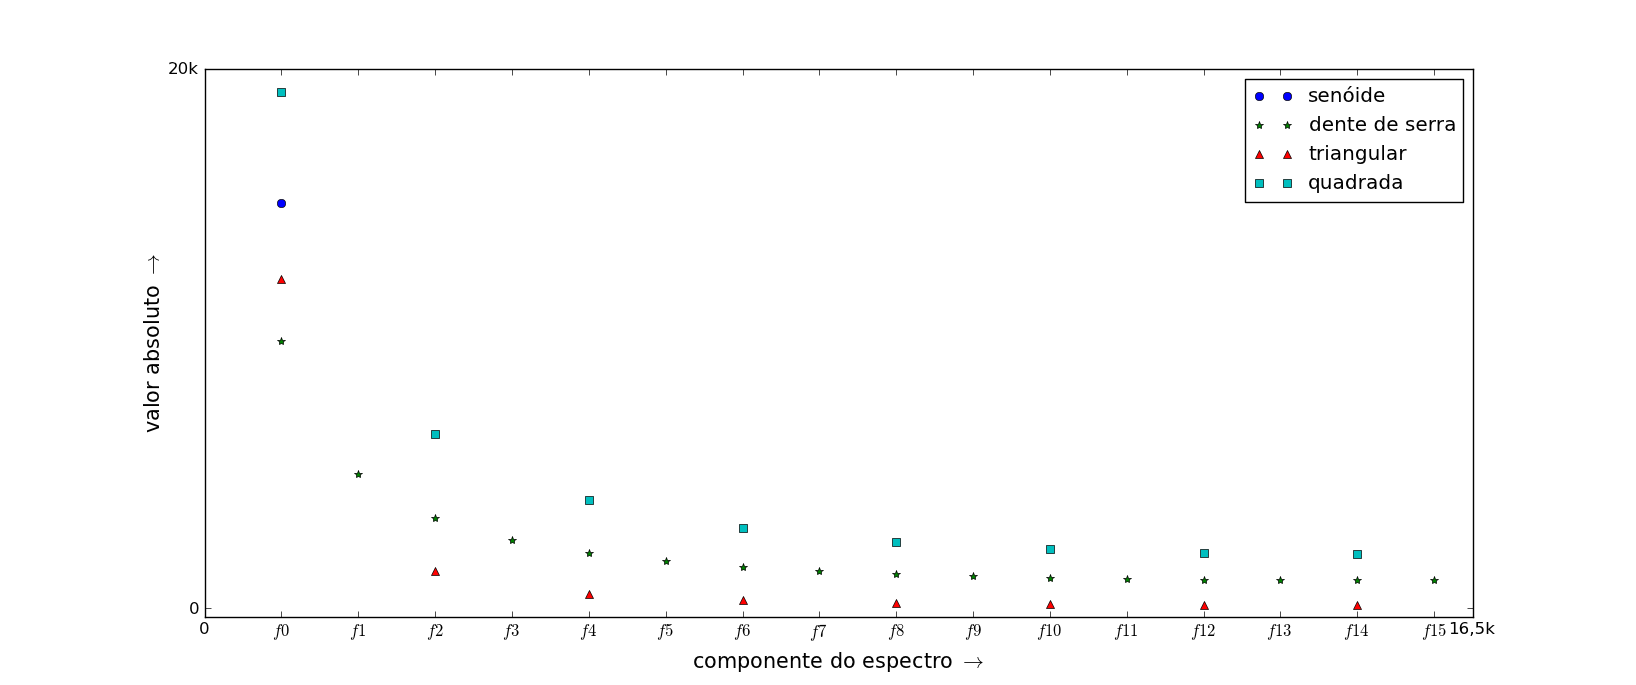
\includegraphics[width=\textwidth]{figuras/espectroDeOndas5b}
        \label{fig:espectroDeOndas}
\end{figure}


O espectro harmônico é formado pelas frequências múltiplas da frequência fundamental $f_n=(n+1).f_0$. Como nossa percepção segue a escala logarítmica, o espectro possui notas diferentes da frequência fundamental. Além disso, o número de harmônicos será limitado pela frequência máxima $f_a/2$. 

Musicalmente crucial aqui é internalizar que a presença de
energia\footnote{A energia total equivale à soma dos quadrados das amplitudes como as de pressao/voltagem pelo tempo, e.g. figura ~\ref{fig:formasDeOnda}.
As componentes espectrais - e.g. ~\ref{fig:espectroDeOndas} e ~\ref{fig:espectroOboe} -
também podem ser elevadas ao quadrado para resultar em quantificação de energia e somam-se na energia total. As energias se equivalem pelo teorema de Parseval.}
em uma componente de frequência $f_n$ na decomposição por fourier 
implica na presença de uma oscilação senoidal na constituição do som, puramente harmônica no som e naquela frequência $f_n$. Esta energia concentrada especificamente na frequência $f_n$ é separada
 pelo ouvido para adentrar em um nível cognitivo de processamento\footnote{Esta separação em frequência é realizada por diversas espécies através de mecanismos similares à cóclea humana.}.
  As componentes senoidais são geralmente as principais responsáveis pela qualidade chamada timbre e, caso não apresentem proporções harmônicas (relações de pequenos números), são ruídos, i.e. não são notas com frequência fundamental como o lá 4 ($440 Hz$) de nossos exemplos. Além disso, nossa noção de altura absoluta em um complexo sonoro é baseada na semelhança do espectro com a série harmônica.

No caso de uma forma de onda fixa (e de tamanho fixo), o espectro é sempre harmônico e estático. Fixada a frequência fundamental (inverso do comprimento da onda), cada forma de onda é composta de proporções específicas das componentes harmônicas e 
quanto maior a curvatura do trecho na forma de onda, maior a contribuição do trecho para a
concentração de energia nos harmônicos agudos.

Podemos ver isso claramente em sons reais. A onda rotulada como 'som real amostrado' na figura ~\ref{fig:formasDeOnda} é um período extraído de um som real relativamente comportado. Ele possuí $\lambda_f=114$ amostras\footnote{Caso também utilizado diretamente em $f_a=44,1kHz$, é um pouco mais grave que os $441 Hz$ das formas de onda artificiais $\frac{44100}{114}=385,84Hz$.}. A onda de oboé foi amostrada de um lá 4 também em $44,1kHz$. O período escolhido para a amostragem é relativamente curto, com 98 amostras corresponde a $\frac{44100}{98}=450 Hz$. Pode-se perceber o espectro rico em frequências do oboé e o espectro mais grave do som real. A figura ~\ref{fig:espectroOboe} 
expõe em conjunto o conteúdo espectral da nota original e o resultante da utilização destas amostras.

Note que, definindo $ R_i=\{ r_i \}_0^{\lambda_f-1}$ a sequência de amostras do som real da figura ~\ref{fig:formasDeOnda},
$R_i$ pode ser tomado como base para um som $T_i^f$ da seguinte forma: 

\begin{equation}\label{sampleandoFormaDeOnda}
     T^f_i=\{ t_i^f \}=\Bigl\{ r_{(i\,\%\lambda_{f})} \Bigr\}
\end{equation}

O som resultante possui o espectro momentâneo do som original. Por ser repetido de forma idêntica,
seu espectro é perfeitamente harmônico, sem os ruídos e variações típicas do fenômeno natural. Isso pode ser visto claramente na figura ~\ref{fig:espectroOboe} onde os espectros da nota original do oboé e de uma nota 
artificial - de mesma duração e cujas amostras consistem no mesmo período da figura ~\ref{fig:formasDeOnda} - estão dispostas juntamente. O espectro natural possui variações na frequência dos harmônicos, nas suas intensidades e uma quantidade de ruído. Já a nota cujo período foi amostrado possui espectro perfeitamente harmônico.



\begin{figure}[h!]
    \centering
    \caption{Espectros das ondas sonoras do oboé natural e de período amostrado}
        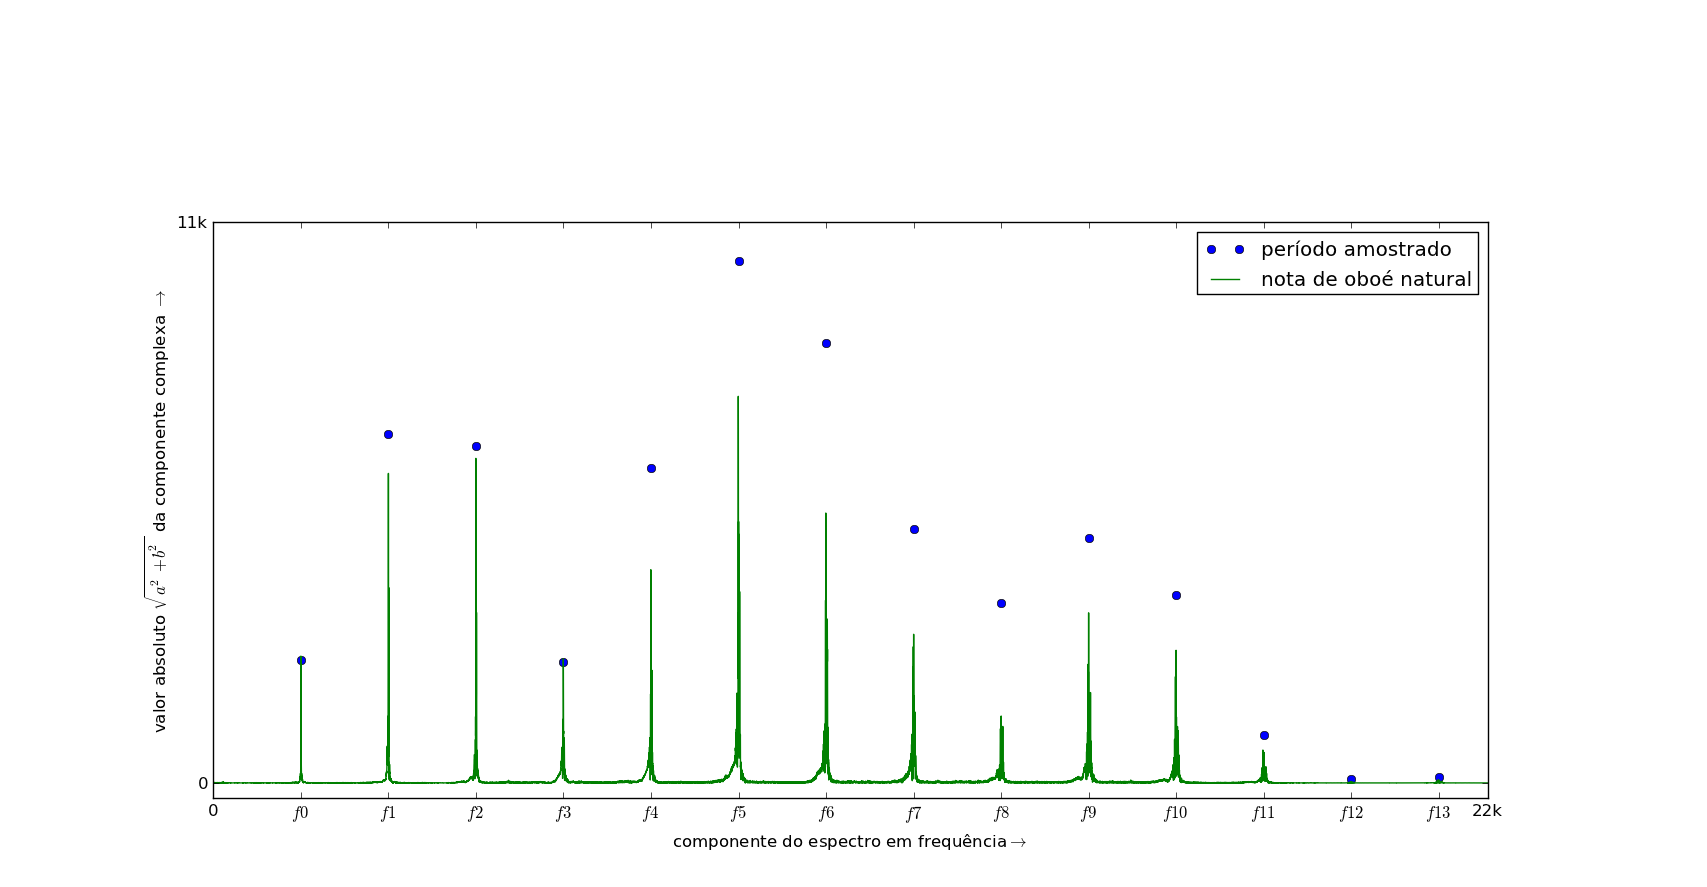
\includegraphics[width=\textwidth]{figuras/espectroOboeAmostradoNatural2}
        \label{fig:espectroOboe}
\end{figure}





\subsubsection{O espectro no som amostrado}
Além deste papel-chave no timbre e na cognição como um todo, a presença e comportamento destas componentes é peculiar no som discretizado. Considere um sinal $T_i$ e sua decomposição de Fourier $\mathcal{F}\{T_i\}=C_i=\{c_i\}_0^{\Lambda-1}$. Sabemos que a recomposição segue a conversão das componentes frequenciais em amostras temporais\footnote{Lembrando que o fator $\frac{1}{\Lambda}$ pode ser distribuído dentre a transformada e a reconstrução como preferir}:

 
\begin{equation}\label{recomposicaoFourier}
t_i = \frac{1}{\Lambda}\sum_{k=0}^{\Lambda-1}c_ke^{j . \frac{2\pi k}{\Lambda} i } = \frac{1}{\Lambda}\sum_{k=0}^{\Lambda-1}(a_k+ j . b_k)\left[cos(w_k i) +j . sen(w_k i)\right]
\end{equation}

Onde $c_k = a_k + j . b_k$ pondera a amplitude e fase de cada frequência $w_k=\frac{2\pi k}{\Lambda}$. Nosso som possui amostras $t_i$ reais que resultam das contribuições de cada componente de frequência $w_k$ e cujo $c_k$ regula o módulo e a fase. A parte real da equação ~\ref{recomposicaoFourier} nos fornece a componente de forma mais clara:

\begin{equation}\label{moduloEfase}
\begin{split}
t_i& = \frac{1}{\Lambda}\sum_{k=0}^{\Lambda-1}\left[a_k cos(w_k i) -b_k sen(w_k i)\right] \\
   & = \frac{1}{\Lambda}\sum_{k=0}^{\Lambda-1}\sqrt{a_k^2 + b_k^2} \; cos\left[w_k i - tg^{-1}\left(\frac{b_k}{a_k}\right)\right]
\end{split}
\end{equation}

Podemos notar claramente pela equação ~\ref{moduloEfase} que o termo imaginário apenas acrescenta uma fase à senóide real. Ao mesmo tempo $b_k$ também altera a amplitude mas a informação de amplitude já está em $a_k$, i.e. os termos imaginários da decomposição espectral por Fourier proporcionam a varredura de fase
 $[-\frac{\pi}{2},+\frac{\pi}{2}]$. O sinal de $a_k$ especifica se estamos do lado direito ou esquerdo do circulo trigonométrico, completando a varredura completa de fase (os intervalos $[-\frac{\pi}{2},+\frac{\pi}{2}]$ e $[\frac{\pi}{2},\frac{3\pi}{2}]$ completam $2\pi$).


\begin{figure}[h!]
    \centering
    \caption{Oscilação de 2 amostras (frequência máxima em qualquer $t_a$)}
        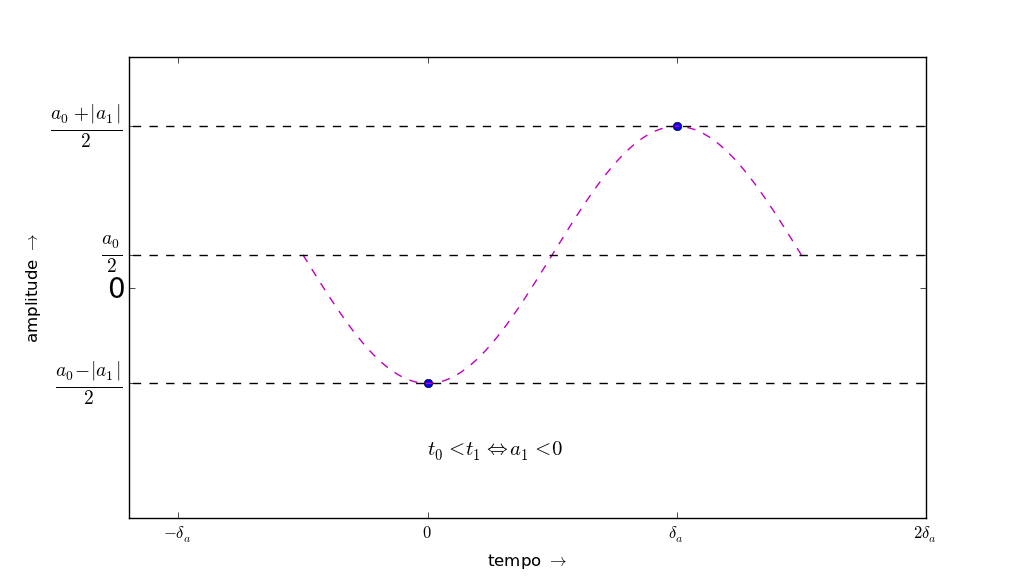
\includegraphics[width=\textwidth]{figuras/amostras2c_}
        \label{fig:amostras2}
\end{figure}

A figura ~\ref{fig:amostras2} exibe duas amostras e a componente espectral que contém. A decomposição de Fourier resulta neste caso em somente dois coeficientes $\{c_k=a_k-j.b_k\}_0^{\Lambda-1=1}$. O papel das amplitudes $a_k$ fica bem claro:
 $a_0$ é o deslocamento fixo\footnote{chamado de bias ou offset} e $a_1$ especifica a amplitude da oscilação em si. A frequência que possui a energia\footnote{Lembrando que as energias garantidamente se equivalem pela $\frac{1}{\Lambda} . \sum_{k=0}^{\Lambda -1}c_k^2 = \sum_{i=0}^{\Lambda-1}t_i^2$ (Teorema de Parseval)}
 $e_k=\frac{(c_k)^2}{\Lambda=2}$ é dada pela relação $f_k=k . \frac{f_a}{\Lambda=2} $.  Ou seja, no caso de duas amostras só temos energia nas frequências $f_0=0$ e $f_1=\frac{f_a}{\Lambda=2}=f_{\text{máx}}$.

Este caso é de especial importância pois o mínimo necessário para representar uma oscilação são 2 amostras e disso resulta a frequência de Nyquist $f_{\text{máx}}=\frac{f_a}{2}$. Esta é a frequência máxima presente em um som amostrado com $f_a$ amostras por segundo\footnote{Qualquer sinal amostrado possui esta característica, não somente o som digitalizado.}.

Vejamos o que acontece no caso de 3 amostras. Todas as sequências fixas $T_i$ de apenas 3 amostras também apresentam
somente 1 frequência, pois sua primeira harmônica usaria 1,5 amostras e ultrapassa o limite inferior de 2 amostras mínimas (a frequência da harmônica ultrapassaria a de Nyquist pois:  $\; \frac{f_a}{3}.2 > \frac{f_a}{2} $). Se $\Lambda=3$, 
os coeficiêntes $\{c_k\}_0^{\Lambda-1=2}$ da decomposição por Fourier apresentam-se em 
3 componentes frequenciais. Uma delas é a frequência zero, as outras duas contribuem de forma igual na reconstrução da senóide com $f=f_a/3$.

\begin{figure}[h!]
    \centering
    \caption{3 amostras apresentam uma única frequência}
        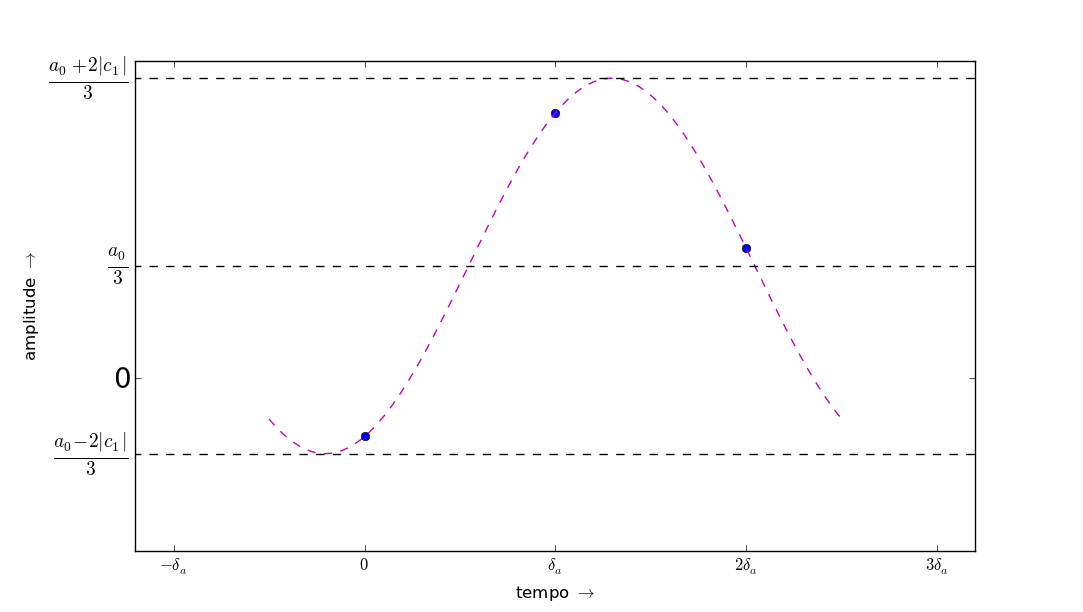
\includegraphics[width=\textwidth]{figuras/amostras3b}
        \label{fig:amostras3}
\end{figure}



Partimos de $\Lambda$ amostras reais $t_i$ e temos $\Lambda$ coeficientes complexos $c_k=a_k+j.b_k$. Os coeficientes $c_k$ se equivalem dois a dois\footnote{Módulos iguais e fases com sinais opostos; $a_{k1}=a_{k2}$ e $b_{k1}=-b_{k2}$.} pois correspondem às frequências $f_k = k.\frac{f_a}{\Lambda}, \; k \in \{0...\Lambda-1\} $
 e quando $ f_k > f_{\text{máx}} = \frac{f_a}{2} $ (o que já exclui $f_0=0$ e $f_k=\frac{f_a}{2}$), a frequência $f_k$ é espelhada para $f_l=\frac{f_a}{2} - (f_k-\frac{f_a}{2})=f_a-f_k=f_a - k\frac{f_a}{\Lambda}=(\Lambda-k)\frac{f_a}{\Lambda} \Rightarrow f_k\equiv f_{\Lambda-k}$. 
 
 O mesmo pode ser observado com 
 $w_k=f_k.\frac{2\pi}{f_a}$ e lembrando da periodicidade $2\pi$, que resulta em $w_k=-w_{\Lambda-k}$. Como o coseno é uma função par e a tangente inversa é impar, as componentes em $w_k$ e $w_{\Lambda-k}$ se somam na equação de reconstrução das amostras reais mostrada em ~\ref{recomposicaoFourier}.

  Dito de outra forma, em uma decomposição de $\Lambda$ amostras, as $\Lambda$ componentes frequenciais $\{c_i\}_0^{\Lambda-1}$ resultantes
   são equivalentes em pares.
   Excepcional excessão para $f_0$ e, no caso de $\Lambda$ ser par, de $f_{\Lambda/2}=f_{\text{máx}}=\frac{f_a}{2}$. Além disso, estas duas frequências (a frequência zero e a frequência máxima) não são representadas com variação de fase e, portanto, são estritamente reais. Assim, podemos 
   concluir que o número $\tau$ de pares de coeficientes equivalentes é:

\begin{equation}\label{coefsPareados}
\tau = \frac{\Lambda - \Lambda \% 2}{2} +\Lambda \% 2 -1
\end{equation}

e resultam evidentes as equivalências ~\ref{equivalenciasFreqs}, ~\ref{equivalenciasModulos} e ~\ref{equivalenciasFases}:

\begin{equation}\label{equivalenciasFreqs}
f_{k}\equiv f_{\Lambda-k}\;, \;\; w_{k}=-w_{\Lambda-k}\;\;\;, \quad \;\; \forall \quad 1 \leq k \leq \tau  
\end{equation}

\begin{figure}[h!]
    \centering
    \caption{Componentes frequenciais em 4 amostras}
        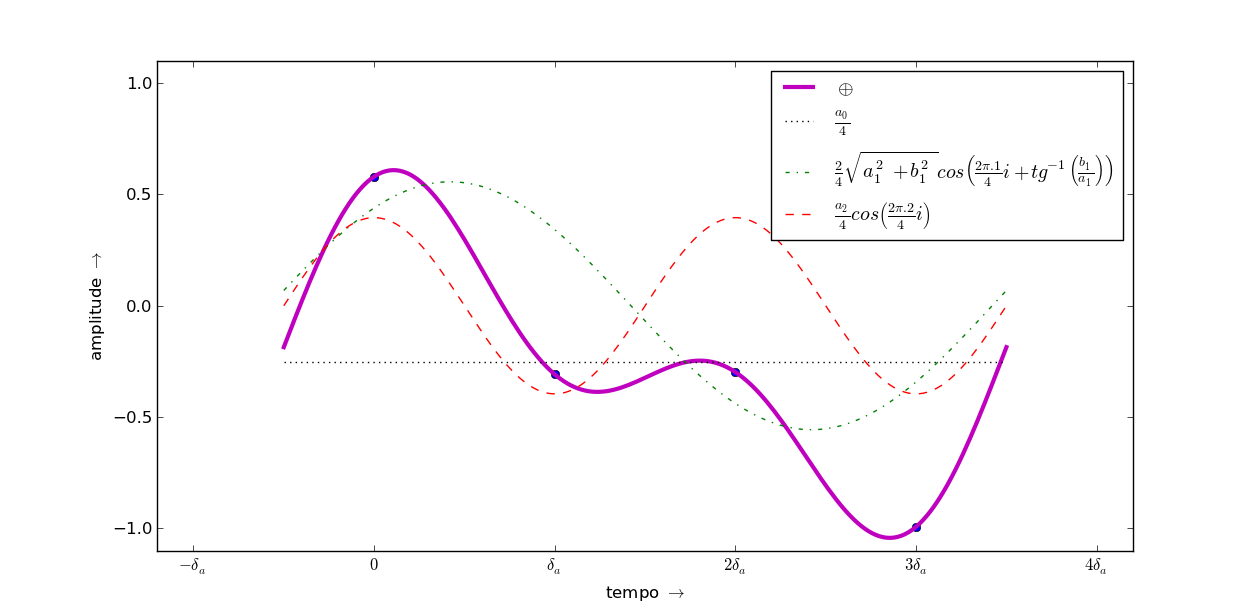
\includegraphics[width=\textwidth]{figuras/amostras4__}
        \label{fig:amostras4}
\end{figure}


Como $a_k = a_{\Lambda -k}\;\;$ e $\;\;b_k = - b_{\Lambda -k}$:

\begin{equation}\label{equivalenciasModulos}
\sqrt{a_k^2 + b_k^2} = \sqrt{a_{\Lambda - k}^2 + b_{\Lambda -k}^2} \;\;, \quad \;\; \forall \quad 1 \leq k \leq \tau  \\
\end{equation}

\begin{equation}\label{equivalenciasFases}
tg^{-1}\left(\frac{b_k}{a_k}\right)=-tg^{-1}\left(\frac{b_{\Lambda -k}}{a_{\Lambda - k}}\right)\;\;,\quad \;\; \forall \quad 1 \leq k \leq \tau
\end{equation}


Com $k \in \mathbb{N}$. A observação da equação de reconstrução para o sinal real ~\ref{moduloEfase} em conjunto com as equivalências dos módulos e fases ~\ref{equivalenciasModulos} e ~\ref{equivalenciasFases}
mostra a combinação em fase das componentes em $w_k$ e $w_{\Lambda-k}$:

\begin{equation}
t_i = \frac{a_0}{\Lambda} + \frac{2}{\Lambda}\sum_{k=1}^{\tau}\sqrt{a_k^2 + b_k^2} \; cos\left[w_k i - tg^{-1}\left(\frac{b_k}{a_k}\right)\right]+ \frac{ a_{\Lambda/2+1}}{\Lambda}.(1-\Lambda\% 2)
\end{equation}

\begin{figure}[h!]
    \centering
    \caption{Formas de onda básicas em 4 amostras}
        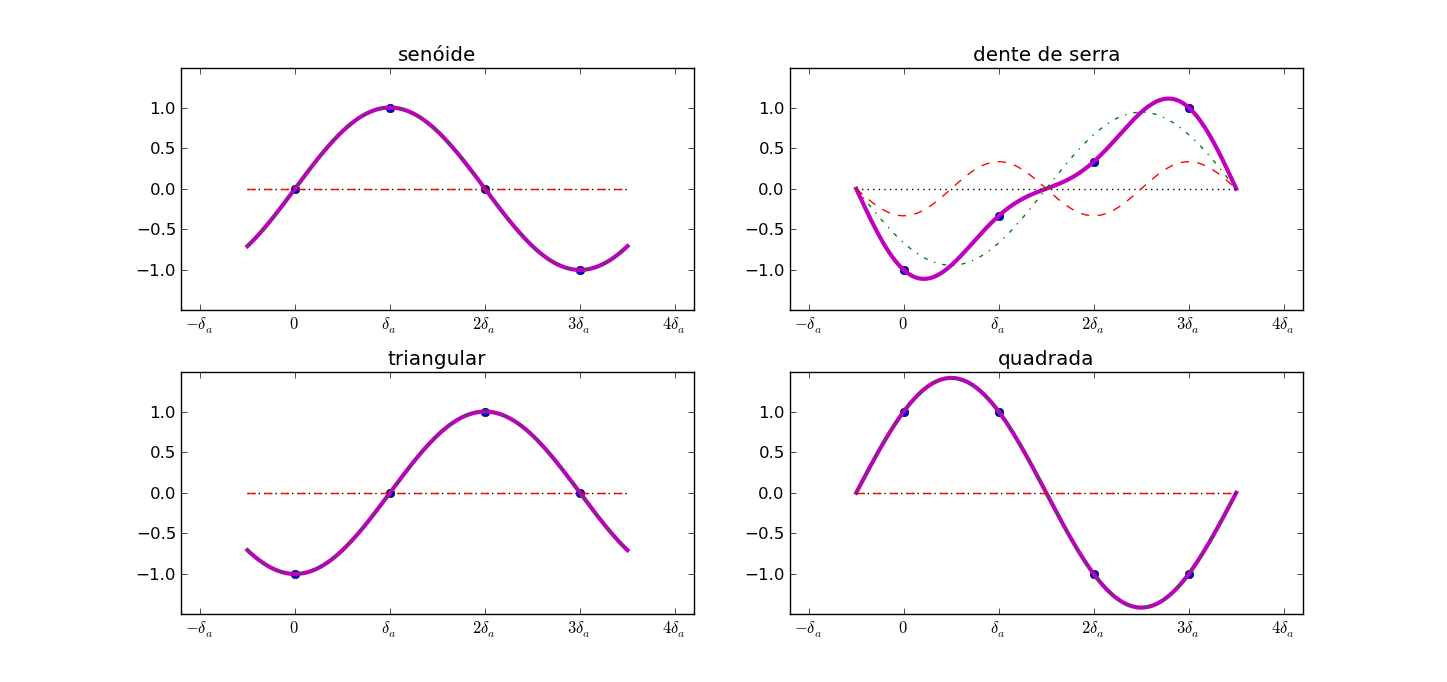
\includegraphics[width=\textwidth]{figuras/amostras4formas__}
        \label{fig:formas4}
\end{figure}


Assim, a exemplo da figura ~\ref{fig:amostras3}, a transformada de Fourier de 3 amostras possui 2 coeficientes imaginários que possuem quantidades iguais de energia na mesma frequência.

Com 4 amostras, podemos representar 1 ou 2 frequências em proporções diferentes. A figura ~\ref{fig:amostras4} mostra uma forma de onda de 4 amostras e suas duas componentes. Note que as contribuições individuais se somam de fato na forma de onda original, e que as curvaturas maiores são fruto da frequência mais aguda.

A figura ~\ref{fig:formas4} explicita os harmônicos em 4 amostras nas formas de onda básicas das equações ~\ref{senoide}, ~\ref{denteDeSerra}, ~\ref{triangular} e ~\ref{quadrada} e figura ~\ref{fig:formasDeOnda}. Todas consistem em apenas 1 senóide, com excessão da dente de serra que possui os harmônicos pares.


A figura ~\ref{fig:amostras6} mostra as decomposições senoidais para o caso de 6 amostras. A figura ~\ref{fig:formas6} decompõe as formas de onda básicas para o caso de 6 amostras.
 Note que neste caso de 6 amostras as ondas se diferenciam espectralmente: as quadrada e triangular possuem as mesmas componentes, mas em proporções diferentes, já a dente de serra possui uma componente a mais.

\begin{figure}[h!]
    \centering
    \caption{Componentes frequenciais em 6 amostras}
        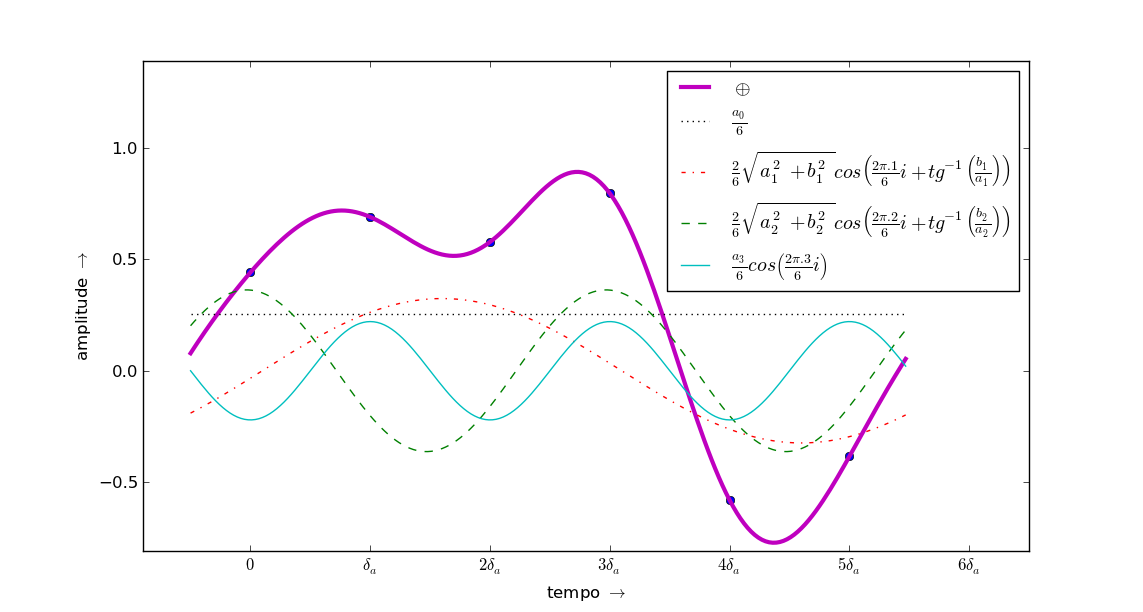
\includegraphics[width=\textwidth]{figuras/amostras6}
        \label{fig:amostras6}
\end{figure}

\begin{figure}[h!]
    \centering
    \caption{Formas de onda básicas em 6 amostras}
        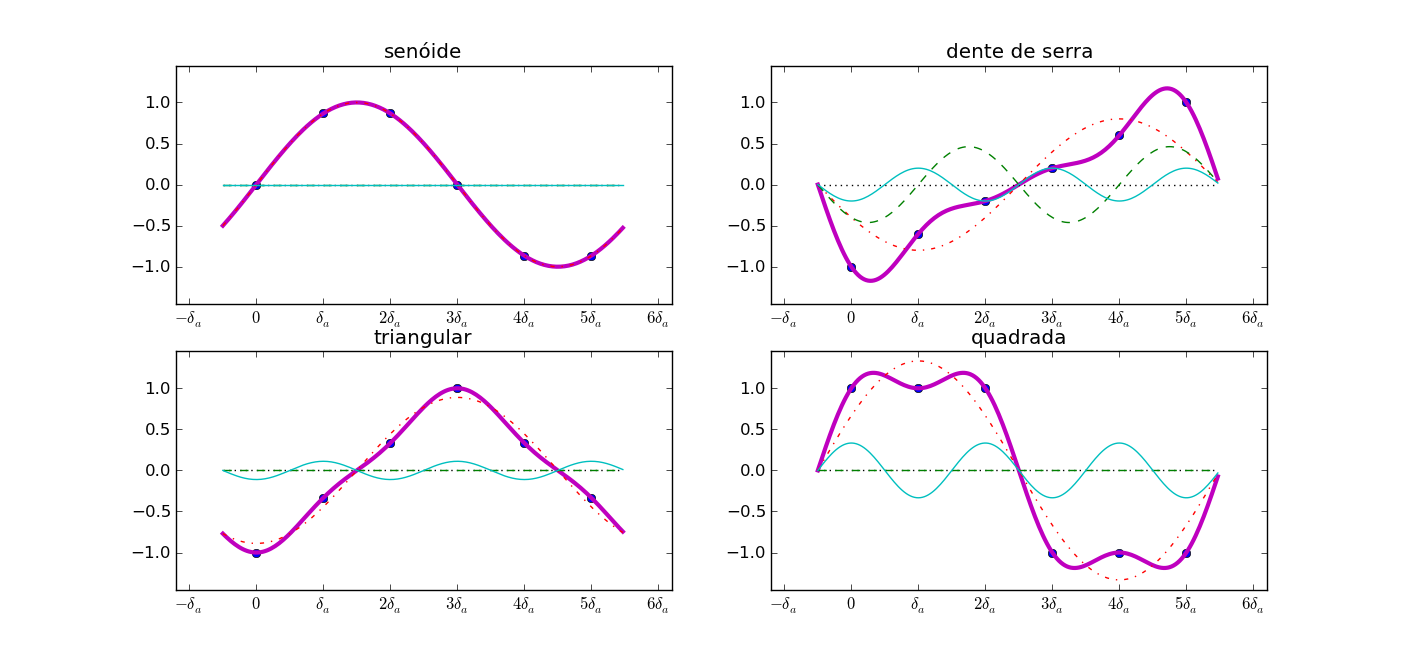
\includegraphics[width=\textwidth]{figuras/amostras6formas___}
        \label{fig:formas6}
\end{figure}

\subsubsection{A nota básica}

Escolhamos $f$ tal que $f$ divida $f_a$  
 \footnote{Esta escolha facilita as demonstrações pois os períodos são quantidades inteiras de amostras. Transporemos esta limitação na prática com o uso de uma tabela de amostragem ou com o uso direto de funções periódicas,e.g. $t_i=sen(x.i)$. Veja próxima sessão.}. 
Uma sequência $T_i$ de amostras sonoras separadas por $\delta_a=1/f_a$ descreve uma nota musical de frequência $f$ Herz e duração $\Delta$ segundos se, e somente se, possuir a periodicidade $\lambda_f=f_a/f$ e tamanho $f_a . \Delta$:

\begin{equation}
T_i^{f,\; \Delta}=\{t_{i \, \% \lambda_f} \}_0^{f_a . \Delta}=\{t_{i \; \% \left( \frac{f_a}{f} \right) } \}_0^{f_a . \Delta}
\end{equation}

Note que a nota por si só não especifica um timbre. Mesmo assim, faz-se necessária a escolha de uma forma de onda para que as amostras $t_i$ tenham um valor estabelecido individualmente. Um único período dentre as ondas básicas pode ser utilizado para a especificação da nota da seguinte forma:

seja $f$ a frequência da nota, $\delta_f=1/f$ o seu comprimento de onda e $L_i^{f,\, \delta_f} $ a sequência que descreve um período da onda $L_i^f \in \{S_i^f,Q_i^f,T_i^f,D_i^f,R_i^f \}$ (ver equações ~\ref{senoide}, ~\ref{denteDeSerra}, ~\ref{triangular} e ~\ref{quadrada}; $R_i^f$ é uma onda real amostrada):

\begin{equation}\label{periodoUnico}
L_i^{f , \delta_f } = \{ l_i^f \}_0^{\delta_f . f_a -1}=\{ l_i^f \}_0^{\lambda_f-1}
\end{equation}

Então a sequência $T_i$ consistirá em uma nota de duração $\Delta$ e frequência $f$ se:

\begin{equation}
T_i^{f,\; \Delta}=\{t_i^f\}_0^{f_a . \Delta}=\{l^f_{i\,\%\left(\frac{f_a}{f}\right)}\}_0^{f_a . \Delta}
\end{equation}


\subsubsection{Usos musicais}

Em posse da nota básica, podemos montar estruturas musicais com
sequências destas partículas. Caso somemos $N$ sequências ($T_{k,i}=\{t_{k,i}\}, \;\; k \in 0...N-1$) de mesmo tamanho, seus conteúdos espectrais serão sobrepostos e a isso damos o nome de mixagem:

\begin{equation}
\{t_i\}=\left \{ \sum_{k=0}^{N-1}t_{k,i} \right \}
\end{equation}

Pode-se completar com zeros para somar sequências de tamanhos diferentes. O resultado da mixagem de notas musicais é a harmonia musical, cujos intervalos entre as frequências e os acordes de notas simultâneas regem aspectos subjetivos e abstratos da música e sua apreciação.

As sequências podem também ser concatenadas no tempo. Caso as sequências $\{t_{k,i}\}_0^{\Lambda_k-1}$ de tamanhos $\Lambda_k$  representem $k$ notas musicais, sua concatenação em $t_i$ resultará em sequências musicais simples ou melodias:

\begin{equation}
\{t_i\}_0^{\sum\Delta}=\{t_{k,i}\}_0^{\sum\Delta}, \;\; k\text{ menor inteiro } : \quad \Lambda_k > i -\sum_{j=0}^{k-1}\Lambda_j
\end{equation}

A montagem musical \emph{reduced-fi} demonstra de forma isolada este uso de justaposição temporal das notas, resultando em uma peça homofônica. O princípio vertical está demonstrado nos \emph{quadros sonoros}, sons estáticos com espectros peculiares. Ambas as peças estão em código Python no APÊNDICE XX e podem ser escutadas e vizualizadas nos links [][][].

Com isso estabelecemos nossa nota musical básica no som digital. Trabalharemos a seguir estas unidades, a evolução temporal de seus conteúdos e desenvolveremos as notas musicais com parâmetros que evoluem no tempo, como glissandos e envoltórias. 
A filtragem de componentes e os ruídos finalizam sobre a constituição da nota musical como unidade isolada. A estruturação musical destas notas é então abordada do ponto de vista das estruturas fora do tempo (como as escalas), trajetórias cíclicas ou que convirjam ou divirjam.

\clearpage

\subsection{Variações na nota musical básica}

Nossa nota musical digital básica está bem definida com os parâmetros:
duração, altura, intensidade (volume) e timbre. Esta é uma modelagem
útil e paradigmática, mas de forma alguma esgota o que entendemos por
uma nota musical.

Em primeiro lugar, as características da nota se modificam no decorrer
da própria nota, i.e. em uma nota real os parâmetros
não são absolutamente fixos. Por exemplo, em uma nota de piano
de 3 segundos, a intensidade tem início abrupto e decaimento progressivo
além de variações do espectro instantâneo, com harmônicos que
decaem antes dos outros e alguns que aparecem com o tempo.
Estas variações não necessariamente são levadas
em conta na síntese sonora, mas constituem-se em guias para a
síntese de sons para usos musicais pois é como eles
se apresentam na natureza\footnote{A regra de ouro
aqui é: para que um som isolado disperte interesse
por si só, faça como que tenha variações internas.}. 

Explorar todas as formas pelas quais estas variações ocorrem está fora
do escopo de qualquer trabalho dada a considerável sensibilidade do ouvido humano
e a complexidade da nossa cognição sonora. Desta forma, apontaremos
recursos primários para estas variações dos parâmetros na nossa nota
básica.

Iniciaremos com uma técnica que não resulta propriamente
em variações internas da nota, mas simplificará esta exposição
sem restringir o escopo, além de ser um notável recurso de otimização
computacional.


\subsubsection{Tabela de Busca}


Mais conhecido pelo termo em inglês, a \emph{Lookup table} (ou simplesmente
LUT), é um procedimento simples que consiste em criar uma tabela
de referência e coletar as amostras destas tabelas segundo a 
necessidade\footnote{Em contraposição ao cálculo das amostras individuais
para cada caso.}. Em nosso caso, usaremos tabelas de busca para os
sons criados, as notas. Assim, estas tabelas são unidimensionais e com
valores reais. Além disso, a tabela consiste nas amostras
de um período de onda, que usamos para sintetizar períodos
de tamanhos diferentes, resultando em frequências diferentes.

O procedimento de busca em tabelas é visto geralmente como um
artifício de otimização. Na música seu uso transcende este
primeiro, facilitando as operações e permitindo que um único
período de onda possa ser usado para sintetizar sons em toda a banda
de frequências audíveis.

Descrevemos esta busca. Seja $\widetilde{\Lambda}$ o tamanho 
da tabela e $\widetilde{L_i} = \{ \widetilde{l}_i \}_0^{\widetilde{\Lambda} -1}$ a tabela de elementos $\widetilde{l_i}$ de um
período de onda qualquer (veja equação ~\ref{periodoUnico}). Uma sequência
$T_i^{f,\Delta}$ com amostras de um som de frequência $f$ e duração $\Delta$
pode ser feita a partir de $\widetilde{L_i}$ da seguinte forma:

\begin{equation}
T_i^{f,\Delta}=\{t_i^f\}_0^{f_a . \Delta-1} = \{ \widetilde{l}_{\gamma_i \% \widetilde{\Lambda} } \}_{0}^{f_a . \Delta-1}\; , \quad \text{onde} \;\; \gamma_i = \left \lfloor i . f \frac{ \widetilde{\Lambda}}{f_a} \right \rfloor  
\end{equation}

Ou seja, dada a tabela de busca, basta termos a sequência de índices corretos
para sintetizar o som. Para o cálculo do inteiro $\gamma_i$, convencionamos
atribuir a ele o maior inteiro menor que $i.f\frac{\widetilde{\Lambda}}{f_a}$.
Esta aproximação introduz um ruído, mas conseguimos que este ruído seja desprezível
mesmo se o tomarmos como o maior inteiro acima da multiplicação
ou se arredondarmos por outros métodos. Além disso, para fins de síntese, em $f_a=44,1 kHz$
 o padrão é usar $\widetilde{\Lambda} = 1024$ amostras, pois já não gera ruído
 relevante no espectro audível.

 A expressão que define a variável $\gamma_i$ pode ser facilmente compreendida da
 seguinte forma: a variável $i$ é acrescida de $f_a$ em $1$ segundo (pela
 definição de $f_a$ e $i$, pois temos $f_a$ amostras $t_i$ em $1$ segundo). Caso a dividamos por $f_a$, teremos $\frac{i}{f_a}$,
fração esta que é acrescida de $1$ a cada $1$ segundo. Multiplicado pelo comprimento da
 tabela $\widetilde{\Lambda}$, teremos $i \frac{\widetilde{\Lambda}}{f_a}$
 que resulta na varredura completa da tabela $\widetilde{L_i}$ em 
 1 segundo com o acréscimo de $\widetilde{\Lambda}$ em $1$ segundo. Por fim,
 se multiplicarmos pela frequência $f$ que queremos, teremos $i . f \frac{\widetilde{\Lambda}}{f_a}$
 que resulta em $f$ varreduras completas da tabela $\widetilde{L_i}$ em $1$ segundo, i.e. a sequência
 resultante apresenta a frequência fundamental $f$.

Importantes considerações: $f$ é qualquer, só há limitantes nas frequências
graves quando o tamanho da tabela $\widetilde{\Lambda}$ não é suficientemente grande para a taxa de amostragem
$f_a$\footnote{Como citado acima, $\widetilde{\Lambda} = 1024$ é suficiente para sintetizar
sequências $T_i^f$ com qualquer $f$ no espectro.}. O procedimento de busca em tabela
é computacionalmente bastante barato, substituindo cálculos por buscas simples (por isso geralmente
é entendido como um processo de otimização). Salvo quando assinalado,
a seguir usaremos este procedimento para todos os casos cabíveis pois
simplifica diversas rotinas e é computacionalmente coerente.


\subsubsection{Variações incrementais de frequência e intensidade}

Segundo revela a lei de Weber e Fechner, nossa percepção tem uma relação logarítmica com
o estímulo que a causa. Mesmo assim, dado o uso, explicitaremos também a variação
linear e começaremos descrevendo esta por razões didáticas.

Em uma nota de duração $\Delta = \frac{\Lambda}{f_a}$, a frequência $f=f_i$ varia de $f_0$ até $f_{\Lambda -1}$
linearmente. Podemos então escrever que:

\begin{equation}\label{freqLinear}
f_i=f_0 + (f_{\Lambda-1}-f_0)\frac{i}{\Lambda-1} \quad ,\quad \quad i \;\in\; \mathbb{N}, \quad i \;\in\; [0,\Lambda-1]
\end{equation}

\begin{equation}\label{indiceLinear}
\gamma_i=\left \lfloor i . f_i\frac{\widetilde{\Lambda}}{f_a} \right \rfloor   =\left \lfloor i  \frac{\widetilde{\Lambda}}{f_a} \left [f_0 + (f_{\Lambda-1}-f_0)\frac{i}{\Lambda-1} \right ] \right \rfloor   \quad ,\quad \quad i \;\in\; \mathbb{N}, \quad i \;\in\; [0,\Lambda-1]
\end{equation}

\begin{equation}\label{serieAmostralLin}
\{t_i^{\;\overline{f_0,f_{\Lambda-1}}}\}_0^{\Lambda-1}=\{\widetilde{l}_{\gamma_i \% \widetilde{\Lambda}}\}_0^{\Lambda-1}
\end{equation}

Desta forma, podemos calcular os elementos $t_i^{\;\overline{f_0,f_{\Lambda-1}}}$
com base no período $\{\widetilde{l}_i\}_0^{\Lambda-1}$. Note que na equação
~\ref{freqLinear}, o termo $f_{\Lambda -1} - f_0$ é o âmbito do contra-domínio de $f_i$
e que $\Lambda -1$ é âmbito do domínio. Como $i$ varre o domínio $[0,\Lambda-1]$ e
temos o deslocamento $f_0$ na imagem, $f_i$ varre o contra-domínio 
na medida em que $i$ varre o domínio\footnote{Estas digressões são importantes
para entendermos o significado musical do comportamento destas sequências de amostras.}.

As equações ~\ref{freqLinear}, ~\ref{indiceLinear} e ~\ref{serieAmostralLin} são relativas à progressão linear
da frequência. Como assinalado, nossa percepção segue a progressão logarítmica:
uma progressão de frequência
\emph{percebida} como linear segue uma progressão exponencial\footnote{Ou,
dito ainda de outra forma, uma progressão geométrica da frequência
é percebido como uma progressão aritmética de alturas}.

Fazendo a varredura com $i$
de $0$ até $\Lambda-1$, podemos dizer que: $f_i=f_0 . 2^{\frac{i}{\Lambda-1} n_8}$ onde 
$n_8=\log_2\frac{f_{\Lambda-1}}{f_0}$ é o número de oitavas entre $f_0$ e $f_{\Lambda-1}$.
De forma que $f_i=f_0 . 2^{\frac{i}{\Lambda-1}\log_2\frac{f_{\Lambda-1}}{f_0}}=
f_0 . 2^{\log_2\left ( \frac{f_{\Lambda-1}}{f_0} \right )^{\frac{i}{\Lambda-1}}}=
f_0 \left ( \frac{f_{\Lambda-1}}{f_0} \right ) ^{\frac{i}{\Lambda -1}}$. Portanto,
nossas equações de referência para a síntese de transições de frequência tidas como
lineares pelo ouvido são:

\begin{equation}
f_i=f_0 \left ( \frac{f_{\Lambda-1}}{f_0} \right ) ^{\frac{i}{\Lambda -1}}
\end{equation}

\begin{equation}\label{indiceExponencial}
\gamma_i=\left \lfloor i . f_i\frac{\widetilde{\Lambda}}{f_a} \right \rfloor   =\left \lfloor i f_0 \frac{\widetilde{\Lambda}}{f_a} \left ( \frac{f_{\Lambda-1}}{f_0} \right ) ^{\frac{i}{\Lambda -1}} \right \rfloor   \;\; ,\quad \quad i \;\in\; \mathbb{N}, \quad i \;\in\; [0,\Lambda-1]
\end{equation}

\begin{equation}\label{serieAmostralLog}
\{t_i^{\;\overline{f_0,f_{\Lambda-1}}}\}_0^{\Lambda-1}=\{\widetilde{l}_{\gamma_i \% \widetilde{\Lambda}}\}_0^{\Lambda-1}
\end{equation}

Onde usamos a equação ~\ref{indiceExponencial} para calcular a sequência $\{\gamma_i\}_0^{\Lambda-1}$ de índices para para
serem buscados na nossa tabela que contém um único período da forma de onda.
Isso é explicitado na equação ~\ref{serieAmostralLog}, onde estabelecemos a relação
 $t_i^{\;\overline{f_0,f_{\Lambda-1}}}=\widetilde{l}_{\gamma_i \% \widetilde{\Lambda}}$.
Note que a equação ~\ref{serieAmostralLog} se mantém (permanece idêntica à equação ~\ref{serieAmostralLin}).

O termo $\frac{i}{\Lambda-1}$ varre o intervalo $[0,1]$ e podemos elevá-lo a uma potência
para que o início da transição seja mais suave ou mais abrupto (compensado pelo final
da transição). Este procedimento é mais comum para o caso de variações de volume através da energia
da onda vibratória\footnote{O aumento do volume pode ocorrer por diversas características, como
a reverberação e a concentração de harmônicos agudos e a energia. A mais facilmente controlada
é a energia da onda (veja equação ~\ref{potencia}) e a energia também pode variar de diferentes formas. A forma mais
simples e conveniente geralmente é a variação de amplitude. A variação de energia sem variação de
amplitude é comumente chamado de \emph{compressão sonora} e é muito útil e corriqueiro na prática
de produção musical atual}. Nestes casos, o procedimento comum é multiplicar a sequência original
(seja ela gerada ou pré-estabelecida) pela sequência $\left ( \frac{i}{\Lambda-1} \right )^\alpha$
onde alpha é o coeficiente citado.

Assim, para variações de amplitude, aplicamos as seguintes fórmulas:

\begin{equation}
\{a_i\}_0^{\Lambda-1}=\left \{ a_0 \left ( \frac{a_{\Lambda-1}}{a_0} \right )^{\left ( \frac{i}{\Lambda-1} \right )^\alpha} \right \}_0^{\Lambda-1}=\left \{ \left ( {a_{\Lambda-1}} \right )^{\left ( \frac{i}{\Lambda-1} \right )^\alpha} \right \}_0^{\Lambda-1} \text{ com } a_0=1
\end{equation}

\begin{equation}
T_i^{'}=T_i \odot A_i = \{t_i . a_i\}_0^{\Lambda-1}=\left \{ t_i . (a_{\Lambda-1} )^{\left ( \frac{i}{\Lambda-1} \right )^\alpha} \right \}_0^{\Lambda-1}
\end{equation}

Nosso intuito aqui é modificar a amplitude de um sinal original, seja qual for ele. Desta forma, tomamos
$a_0=1$ para iniciar a nova sequência com a amplitude original e então ir modificando com o decorrer das amostras.
Esta restrição faz com que nosso termo $a_{\Lambda-1}$ seja efetivamente a variação da amplitude.
Caso $\alpha=1$, a variação de amplitude segue exatamente a progressão geométrica que caracteriza
a percepção linear.

Para resultar em uma amplificação linear, basta usarmos umas série $\{a_i\}$ diferente:

\begin{equation}
a_i=a_0 + (a_{\Lambda-1}-a_0)\frac{i}{\Lambda-1}
\end{equation}

Com $a_0=1$ para preservar a amplitude inicial original.

Aqui pode muito nos auxiliar a conversão de decibeis para amplitude apresentada na equação ~\ref{ampDec},
resultando em:

\begin{equation}
T_i^{'}=\left \{ t_i . (10^{\frac{V_{dB}}{20}} )^{\left ( \frac{i}{\Lambda-1} \right )^\alpha} \right \}_0^{\Lambda-1}
\end{equation}

para o caso geral de variações de amplitude segundo a progressão geométrica.


\subsubsection{Tremolo e Vibrato}

Enquanto o vibrato é uma variação periódica de altura (frequência),
o tremolo é uma variação periódica de volume (intensidade).

Iniciemos pelo vibrato. Para realizarmos o caso mais geral, façamos uma sequência $t_i'$
de frequência $f'$ com o auxílio
de uma segunda tabela $\widetilde{M}_i$ de tamanho $\widetilde{\Lambda}_M$ que apresente também
um período de onda que oscila entre $[-1,1]$. Descrevemos uma sequência $t_i^{vbr(f')}$ com
um vibrato de frequência $f'$ e profundidade  $\mu$ (quantos herz é a oscilação no pico superior)
ou $\nu$ (quantos semitons) da seguinte forma:


\begin{equation}\label{vbrGamma}
\gamma_i'=\left \lfloor i f' \frac{\widetilde{\Lambda}_M}{f_a} \right \rfloor
\end{equation}

\begin{equation}\label{vbrAux}
t_i'=\widetilde{m}_{\gamma_i' \;\% \widetilde{\Lambda}_M}
\end{equation}

\begin{equation}\label{vbrF}
f_i=f \left ( \frac{f + \mu }{f} \right )^{t_i'}=f . 2^{t_i'\frac{\nu}{12}}
\end{equation}

\begin{equation}\label{vbrGamma}
\gamma_i = \left \lfloor i . f_i \frac{\widetilde{\Lambda}}{f_a} \right \rfloor = \left \lfloor i \frac{\widetilde{\Lambda}}{f_a}f \left ( \frac{f + \mu }{f} \right )^{t_i'}  \right \rfloor= \left \lfloor i \frac{\widetilde{\Lambda}}{f_a}f . 2^{t_i'\frac{\nu}{12}}  \right \rfloor
\end{equation}

\begin{equation}\label{vbrT}
T_i^{f, vbr(f')}=\{ t_i^{f,vbr(f')} \}_0^{\Lambda-1}=\{ \widetilde{l}_{\gamma_i \%\; \widetilde{\Lambda} } \}_0^{\Lambda-1}
\end{equation}


Para a correta realização do vibrato, é importante atenção para as duas tabelas e sequências.
A tabela $\widetilde{M}_i$ de tamanho $\widetilde{\Lambda}_M$ e a sequência de índices $\gamma_i'$ formam a sequência $t_i'$
 que é o padrão da oscilação da frequência enquanto
a tabela $\widetilde{L}_i$ de tamanho $\widetilde{\Lambda}$ e a sequência de índices $\gamma_i$ formam $t_i$ que é o som em si.
As variáveis $\mu$ e $\nu$ quantificam a intensidade do vibrato: $\mu$ é uma medida direta da quantidade
de Herz envolvidos no limite superior da oscilação e $\nu$ é a medida direta de semitons envolvidos na oscilação.
Note que $\nu=\log_{2}\frac{f+\mu}{f} $ é conveniente neste caso pois o aumento máximo de frequência
não equivale à diminuição máxima, mas a variação de semitons se mantém.

O caso do tremolo é semelhante e $f'$, $\gamma_i'$ e $t_i'$ permanecem os mesmos. Calculamos
a sequência de amplitudes a serem multiplicadas pela sequência original $t_i$ da
sequinte forma:

\begin{equation}\label{trA}
a_i=10^{t_i' \frac{V_{dB}}{20}} = a_{\text{máx}}^{t_i'}
\end{equation}

\begin{equation}\label{trT}
T_i^{tr(f')}=\{ t_i^{tr(f')} \}_0^{\Lambda-1}=\{ t_i . a_i \}_0^{\Lambda-1}=\{t_i .10^{t_i' \frac{V_{dB}}{20}}    \}_0^{\Lambda-1}=\{t_i . a_{\text{máx}}^{t_i'}\}_0^{\Lambda-1}
\end{equation}

Onde $V_{dB}$ é profundidade da oscilação em decibeis do tremolo e $a_{\text{máx}}$ é o ganho máximo de amplitude envolvido.
A medição em decibeis é bastante conveniente neste caso pois o aumento máximo de amplitude
não equivale à diminuição máxima relacionada, enquanto a diferença em decibeis se mantém.

Com as equações ~\ref{vbrT}, ~\ref{vbrGamma}, ~\ref{vbrF}, ~\ref{vbrAux} e  ~\ref{vbrGamma}
são utilizadas para síntese de frequência modulada (FM) nos casos em que $f'$ é
maior que $20Hz$ onde as oscilações de frequência resultam em padrões complexos
de componentes espectrais harmônicas e não harmônicas. As equações ~\ref{trA}
e ~\ref{trT} (junto às ~\ref{vbrT} e ~\ref{vbrGamma} para a realização da sequência
auxiliar $t_i'$) resultam na síntese de amplitude modulada (AM)\footnote{As sínteses
FM e AM são técnicas com diversas amplicações na música e também em outras áreas,
especialmente conhecidos são os usos telecomunicações para transferência de informações
via ondas eletromagnéticas. O leitor interessado pode visitar os itens relacionados
da nossa bibliografia para uma abordagem musical (veja especialmente ~\ref{} e ~\ref{})}.

\subsubsection{Filtros}
O recurso básico para modificar a contribuição das componentees espectrais
na composição de um som é a filtragem. Os filtros proporcionam
ganhos e atenuações diferentes para porções diferentes do espectro,
possibilitando que haja diminuição ou remoção de ruídos e modificações
de timbres quando desejável. A aplicação de filtros pode
ser parte constituinte da síntese ou poder ser feita posteriormente
como parte dos processos tipicamente chamados de tratamento sonoro.
No estudo de filtros, a concepção usual é a de multiplicação de espectros
(espectro do som multiplicado pelo espectro do filtro).

É importante frizar que a elaboração de filtros
constitui uma área reconhecidamente complexa, com literatura
e pacotes de software dedicados. Desta maneira, o texto a seguir
é um resumo do que é utilizado na prática e de forma alguma cobre
todas as possibilidades. Apontaremos utilizações destes filtros junto
às especificações.

\begin{itemize}

\item Filtros de resposta ao impulso finita (FIR)

Esta classe de filtros é conhecida
pela sua sigla FIR (do inglês Finite Impulse Response)
e é caracterizada por possuir uma representação amostral
finita. Esta representação amostral é chamada
de 'resposta ao impulso'. Os filtros FIR são aplicados ao som
digitalizado pela convolucão do som com sua representação
amostral:

\begin{equation}
convolucao\;de\;filtro\;fir
\end{equation}

Importante aqui é notar a vantegem e desvantagem do filtro FIR.
Podemos especificar a filtragem intensionada através do perfil
espectral a ser multiplicado pelo espectro que do som. Através da transformada
de Fourier inversa, obtemos a resposta ao impulso. Assim,
filtros FIR permitem que apliquemos os filtros exatos
que desejarmos.

\item Filtros de resposta ao impulso infinita (IIR)

A exemplo dos filtros FIR, esta classe de filtros é
conhecida pela sigla IIR (do inglês Infinite Impulse Response)
e é caracterizada por possuir uma representação amostral (resposta
ao impulso) infinita. Sua aplicação é usualmente feita pela equação
a diferenças:

\begin{equation}
equacao\;a\;diferencas\;filtro\;iir
\end{equation}

Como pode ser notado, os filtros IIR são muito mais requerem
menos processamento computacional para serem aplicados. Além disso,
podem ser aplicados com maior localidade. Por este motivo, são os mais usuais
para aplicações em geral, mas a obtenção de filtros IIR com características
desejadas muitas vezes revela-se uma tarefa nada trivial\footnote{Encorajamos
o leitor interessado a visitar nossa bibliografia, em especial os livros
~\ref{} e ~\ref{}.}.

\end{itemize}

Os fitros possuem ainda uma segunda classificação,
conforme o perfil espectral que aplicam. A seguir
apontamos os tipos mais cruciais para a prática musical.

\begin{enumerate}
\item Passa-baixas

\item Passa-altas
\item Passa-banda
\item Rejeita-banda
\item Nó
\end{enumerate}



\subsubsection{Ruídos}

\subsubsection{Usos musicais}



\subsection{Organização de notas musicais em música}



\clearpage


\section{Áudio e Música (deprecated)}

Por razões didáticas, dividimos este capítulo em 4 partes: música em tempo diferido (ou seja, que não é feito em tempo real),
música em tempo real,  música na matéria (suporte físico em hardware) e música no tecido social
(considerando especialmente as mobilizações humanas relacionadas).

Com isso desejamos expor a prática musical através do código
com exemplos reais de aplicação e em uso pelo autor, por membros do LabMacambira.sf.net,
por parceiros, colaboradores e por usuários eventuais das naturezas mais diversas.

  \subsection{Música em Tempo Diferido: Minimum-fi e FIGGUS}

\begin{quotation}
\small
'The increasing dominance of graphic interfaces for music software obscured 
the continuing presence of the command-line tradition, 
the code writer, the hacker. The code writing of deferred time 
computer programming may be assembled out of time order, debugged and optimized.'

\emph{Simon Emmerson, Living electronic music, 2007}
\end{quotation}

A realização musical em tempo diferido é o paradigma inicial da música computacional.
Iniciando com o Music V, a proposta foi depois desenvolvido com o CSound. Pode-se dizer
que até hoje é a forma como compositores usualmente pensam a música: pensando
e escrevendo as estruturas, que depois são executadas por instrumentistas ou aparelhos eletrônicos.

Assim como a composição instrumental permite um trabalho mais minucioso do que
a improvisação instrumental, a realização musical em tempo diferido usualmente permite um
detalhamento maior dos procedimentos do que a realização em tempo real. Por este
mesmo motivo, trataremos inicialmente de dois trabalhos em tempo diferido.
Aliás, como veremos a seguir, as abordagens completam uma base para a música
computacional praticada até os dias de hoje.

O som musical pode ser caracterizado físicamente, e sua síntese digital com base em nossa banda de audição e no teorema de Nyquist, sintetiza uma música amostra por amostra, através de princípios
claros de síntese sonora e organização musical\footnote{Veja no APÊNDICE XX: o \emph{minimum-fi} hi-fi, low-fi, minimum-fi, ou seja,
o mínimo de qualidade para assegurar existência e consistência
da criação}. O segundo, chamado de \emph{FIGGUS} (FInite
Groups in Granular and Unit Synthesis), utiliza os princípios do minimum-fi e constitui
um módulo Python completo, cuja proposta é a utilização de simetrias, através de
permutações e de Teoria de Grupos, para a composição de músicas. Como demonstração
das capacidades do FIGGUS, ele gera um EP\footnote{Extended Play, uma album musical maior que um single mas menor que um LP (Long Play) inteiro} com um único comando. Este é o
\emph{PPEPPS}\footnote{Pure Python EP: Projeto Solvente}, como veremos a seguir.

Desta forma, esta sessão exemplifica e explicita - através de dois exemplos reais - os
princípios do uso de código para a síntese \emph{musical}, desde as amostras
relativas a uma nota com dada frequencia, amplitude e timbre, até a confecção
de uma ferramenta derivada, já incorporando propostas musicais e estruturas
mais elaboradas.

      \subsubsection{Minimum-fi}

Existe uma perene matiz estética e também tecnológica
de realizar uma dada tarefa com \emph{o mínimo} necessário.
Esta matiz é para a música igualmente
fundamental e reconhecida como
princípio de unidade e coerência\footnote{Este princípio tanto é fundamental
que as escolas musicais possuem técnicas específicas, músicas possuem suas
próprias convenções mantidas por toda a sua duração, os arcos mantém características,
enfim, podemos até mesmo concluir que a simetria define o escopo.}. Em código computacional
a empreitada para manifestar este princípio ele próprio de forma mínima
resultou no \emph{minimum-fi.py}, código Python em um único arquivo curto que sintetiza
músicas com segundo as estruturas especificadas em linha\footnote{Em música se fala da \emph{bula} (que equivaleria
às funções em si e das especificações da linguagem) e a partitura ou 'música' propriamente ditas (que equivale à .}.
Na versão atual, de 2012 mas adiantada em 2011, os algorítmos 
em Python propriamente ditos somam 
53 linhas e inclui 5 funções. Com estas funções, estruturas musicais podem 
ser criadas padrão a padrão, nota a nota, amostra por amostra. Na prática e posto em
linguagem cotidiana, resultam em notas que formam
blocos e estruturas hierarquicamente superiores.


Os princípios, bastante simples\footnote{Osvaldo Lacerda, em seu livro \emph{Compendio de Teoria Elementar da Musica} fala das propriedades do som musical de forma equivalente.}, são:
\begin{itemize}
  \item Deve-se ter um mecanismo de síntese sonora que
possibilite a geração de unidades sonoras com diferentes timbres, controle sobre a frequência fundamental e duração específica\footnote{Também entra aqui o volume, mas como o que controlamos de fato é a intensidade relativa entre as notas, resolvemos por bem omitir
esta parte até que fiquem claros os códigos relativos a isso, logo abaixo.}.
  \item Deve-se ser capaz de construir não só unidades sonoras, mas também séries de unidades, sejam sobrepostas (acordes, por exemplo)
  ou justapostas (melodias, por exemplo).
\end{itemize}

Para o primeiro item, se prestam comumente os procedimentos de busca em tabelas/vetores com formas
de ondas em alta resolução (chamado \emph{lookup table}). O procedimento é barato e de qualidade alta
(não acrescentam ruídos relevantes ao sinal).

Para realizarmos a busca de forma eficiente, precisamos de tabelas que contenham cada uma
uma forma de onda. As tradicionais são a senóide e as ondas quadrada, triangular e dente de serra.
Mostramos a seguir estas formas de onda e também uma forma de onda retirada de um som real.

De posse destas formas de onda, A seguir está o procedimento da lookuptable:

\code{Procedimento de Lookup Table}{python_snippets/lookuptable.py}

O primeiro ponto importante é a tabela em si, usualmente unidimensional. É de comum conhecimento que
tabelas com 1024 são mais que suficientes para os usos musicais e a diferença
de qualidade (relação sinal/ruido) não muda consideravelmente com a utilização
de tabelas maiores. A seguir dispomos algumas destas tabelas, mais 
especificamente, dispomos as tabelas para os formatos de onda mais usuais. 

\code{Formas de Onda Tradicionais}{python_snippets/formasDeOnda.py}

Através da utilização do lookup sucessivo (procura-se um valor na primeira tabela
e este valor indica o valor na segunda tabela a ser utilizado), executamos
um waveshaping. Este procedimento é bastante apreciado pela simplicidade e eficácia
na síntese de tímbres diversos e ricos em harmônicos e evolução temporal. Embora
uma explicação exaustiva do waveshaping fuja ao escopo deste trabalho, este
método se caracteriza pela aplicação de uma função não linear ao sinal de entrada.
Neste caso o sinal de entrada é gerado pelo primeiro lookup, a função não linear aplicada
é representada pela segunda tabela e aplicada pelo segundo lookup.

Existem muitas formas de se executar waveshaping, a seguir segue o que usamos no minimum-fi, que se sustenta principalmente por ser leve e simples:

\code{Waveshaping com Lookups sucessivas}{python_snippets/lookup_cruz.py}

O segundo item - dos dois princípios expostos sobre o minimum-fi - presta-se à discretização do espaço musical. Unidades como batidas e notas
tornam mais eficiente a comunicação pois a quantidade
de estruturas sugeridas é maior e as estruturas são mais claras no discreto do que no contínuo~\cite{Roederer}. Roederer chega a
apontar que as próprias notas dos instrumentos musicais são um reflexo de que é mais eficiente
o uso do discreto do que do contínuo para a geração de estruturas musicais.

De fato, unidades bem definidas se mostram úteis na prática musical 
para fazer sequências de unidades, concatená-las. Quando as unidades
são notas, as sequências de unidades justapostas no tempo são melodias ou linhas melódicas. As
sequências sobrepostas no tempo são comumente pensadas como acordes, mas podem ser tidas simplesmente
como sobreposições circunstanciais de duas linhas melódicas. Isso, claro, segundo
a sistematização clássica e usual da música~\cite{Lacerda}\footnote{Vole assinalar aqui que a música do século XX apresentou diversos modelos teóricos que quebram com este entendimento simplificado sobre a música, suas unidades básicas e estruturas relacionadas}.

As duas construções básicas explicitadas a seguir, baseadas na dicotomia melodia/harmonia
(horizontalidade/verticalidade, justaposição/sobreposição), são
as funções \emph{fazSequencia} e \emph{fazAcorde} no minimum-fi. Vale notar elas são absolutamente 
equivalentes em uma análise puramente conceitual, i.e. uma delas pode ser omitida segundo algumas teorizações. Isso fica particularmente óbvio quando se nota que os procedimentos de mixagem e concatenação são
plenamente capazes de realizar o que estas funções realizam. Aliás, as funções nada
mais são do que usos típicos e quase caricatos destes procedimentos: no fazAcorde a mixagem
sobrepõe no tempo todas as unidades, no fazSequencia as unidades são todas juntapostas no tempo.

Como pode-se notar a seguir, as sequências de notas e os acordes, em última instância, são utilizações específicas das 2 funções de síntese sonora explicadas anteriormente: lookup e lookupcruz.

\code{Realização de Sequências de Notas}{python_snippets/fazSequencia.py}

\code{Realização de Acordes de Notas}{python_snippets/fazAcorde.py}

A última das cinco funções utilizadas é uma soma amostra a amostra de dois sons. Para isso,
é necessário completar com zeros a sequência com o menor número de amostras para somar rapidamente:

\code{Somador (função auxiliar)}{python_snippets/somador.py}

Depois disso é usufruir com estruturas criadas. Por exemplo: depois de construidas
algumas tabelas para serem usadas como diferentes timbres, pode-se criar as
escalas completamente simétricas na oitava cromática assim:

\code{Escalas Completamente Simétricas (na grade dos 12 semitons e no âmbito da oitava)}{python_snippets/escalas_simetricas.py}

% escala\_1=range(12) # cromática ascendente sem inclusão da oitava
% escala\_2=range(0,12,2) # tons inteiros
% escala\_3=range(0,12,3) # diminutão
% escala\_4=range(0,12,4) # terças maiores
% escala\_6=range(0,12,6) # trítonos
% \end{python}
% \input{py}

Sendo cada unidade um semitom. Ou seja, cada unidade é o fator que fica presente na conta $f_0 . 2^{(1/12)} . fator $ e resulta na frequência exata da nota relativa a $f_0$ em um sistema temperado ideal.

Podemos também utilizar as usuais
escalas tonais maior e menor natural, harmônica e melódica:

\code{Escalas diatônicas tonais (maiores e menores)}{python_snippets/escalas_Mm.py}

A utilização de intervalos menores que o semitom\footnote{Prática também conhecida
como \emph{microtonalismo}, que gera/utiliza \emph{microtonalidade}.} mostra-se trivial em
nossa implementação. Basta representar sequências de fracionários
que são partes linearmente proporcionais dos semitons ou modificar o fator $f$:

\code{Escalas Microtonais (com quartos e oitavos de tom e intervalos menores)}{python_snippets/escalas_microtonais.py}

Da mesma forma, as triades maiores e menores
são especificadas com simplicidade. Note que aos acordes \emph{diminutão} e
\emph{aumentado} correspodem as mesmas notas das escalas simétricas de terças menores
e maiores respectivamente:

\code{Acordes anotados como listas em python}{python_snippets/acordes.py}


E séries/sequências podem ser anotadas junto a variações:

\code{Séries diversas}{python_snippets/series.py}

Com este arcabouço, o passo seguinte é sintetizar e mixar, resultando
em sequências musicais. A síntese de sequências e acordes são feitos tipicamente
através de comandos desta forma:

\code{Sintetizando sequências e acordes}{python_snippets/seqs_acordes.py}

Já a síntese de estruturas compostas (p.ex. sequências de acordes e sobreposição
de linhas melódicas), são feitas com os recursos usuais da liguagem. Neste caso
usamos listas em Python e implementações em Numpy (mais eficientes em tempo de
execussão e também na simplicidade do código) estão no apêndice. Estes mesmos
procedimentos são praticamente os mesmos em Scilab, C/C++, Javascript, PHP, etc.

A seguir demonstramos para fins didáticos, a construção de acordes periódicos em
python puro\footnote{A implementação não didática destas três linhas de código
podem ser agrupadas em uma só linha.}:

\code{Acordes periódicos}{python_snippets/acordes_periodicos.py}

Em posse destas sequências, acordes e recursos da linguagem,
formamos estruturas hierarquicamente superiores
através da concatenação de estruturas, da mixagem de estruturas, e da amplificação
(ou atenuação) seletiva das mesmas:

\code{Amplificação e mixagem}{python_snippets/amp_mix.py}

Neste ponto, basta criarmos músicas e sequências de interesse estético ou para pesquisa. Dado o ferramental, os encadeamentos dependem de intensões estéticas, entendimentos musicais e estruturas abstratas que mantém a coerência e interesse em uma peça musical. Para o leitor mais interessado, deixamos para o Apêndice X um exemplo de música feita com o minimum-fi. A seguir utilizamos esta base apresentada para sintetizar estruturas musicais e então um EP.

\vspace{10 mm}

        \subsubsection{FIGGUS: FInite Groups in Granular and Unit Synthesis}

Em coerência com os conhecimentos
e tecnologias já apresentados nesta exposição\footnote{Especificamos o arcabouço para geração de sons musicais em unidades
e estruturas compostas logo acima na subsessão sobre o minimum-fi.}, introduzimos agora
um foco especial nas estruturas musicais
desenvolvidas. São elas, inseridas em um momento histórico e
executadas por instrumentos específicos com as técnicas de época,
que constituem uma linguagem musical e músicas propriamente
ditas[ref]. O FIGGUS constitui uma técnica composicional
manifestada em software como ferramenta de síntese de
estruturas musicais por estruturas matemáticas específicas
para representação de simetrias.

Este desenvolvimento foi iniciado em 2006 com o físico-matemático Prof. Adolfo Maia Junior - bem anterior
ao nascimento do minimum-fi - para
tratar de simetrias na música com vistas à composição musical através
de métodos matemáticos\footnote{Duas iniciações científicas trataram do assunto, convenios XXX e YYYY.}. Mais especificamente, a proposta resultou em
um programa voltado para a síntese
granular e síntese de estruturas musicais através de Grupos Algébricos. O nome dado
foi FIGGUS, sigla de FInite Groups in Granular and Unit Synthesis\footnote{Também utilizamos
o nome FIGGS (FInite Group in Granular Synthesis) dado que o termo \emph{unit synthesis} não
é usual na literatura. Posteriormente o primeiro autor deste trabalho recorreu novamente
ao uso do nome FIGGUS. Isso foi motivado principalmente pelo fato de que
o maior uso da técnica é para síntese de estruturas musicais, não para
síntese de amálgamas sonoros (ou timbres mesmo) tipicamente resultantes da síntese granular}.

Na atual reescrita, embora ainda bastante atrás do FIGGUS original quanto
à interface gráfica, a ferramenta opera diretamente em Python puro,
com as biblitecas imbutidas por padrão. Isso permite com que o FIGGUS
sintetize todo um EP usando somente os comandos:

\code{Utilizando o FIGGUS para Sintetizar um EP}{python_snippets/synth_ep.py}

Desta forma, a ferramenta fica muito mais simples para experimentações
e implementações adicionais pois sua utilização se dá através
do próprio código no qual tudo é especificado. Esta abordagem se mostra particularmente
pertinente pois a estagnação do mecanismo de síntese de estruturas musicais
beira a inviabilização do uso artístico ou torna necessário o uso
de recursos externos.
Outro uso pretendido para o FIGGUS
é a síntese de tímbres e amálgamas sonoros através da
Síntese Granular. Embora nosso foco seja outro, cabe algumas breves
palavras sobre o assunto.

A Síntese Granular é uma área bem estabelecida tanto na acústica quanto
na Computação Musical e se caracteriza pela geração de sons bastante curtos
e em quantidade massiva. Tipicamente os sons possuem entre 5 e 40 milissegundos
e a quantidade destes \emph{microsons}\footnote{Grãos sonoros e microsons são jargões
típicos da síntese granular usados para indicar sons com as durações especificadas
no texto.} pode chegar a milhares por segundo. O tratamento específico da
síntese granular foge ao escopo deste trabalho e indicamos ao leitor interessado
os artigos produzidos sobre Síntese Granular e Teoria de Grupos[refs AES e SBCM].
Assim, focamos o texto a seguir em Grupos Finitos e Síntese de Estruturas Musicais.

Nas artes é de comum conhecimento o papel absolutamente central
que as simetrias possuem. Na música, para citar somente alguns exemplos simples,
temos os numerosos estudos de simetrias na música de J. S. Bach, os jogos
de dados de Mozart e os usos recorrentes da proporção áurea na música
de Béla Bártok. Matematicamente, as \emph{simetrias} são descritas por Grupos,
e estes são definidos como sendo um conjunto (chamemos de $G$)
munido de uma operação (seja $\bullet$), formando um grupo $(G,\bullet)$
satisfazendo as seguintes propriedades:

\begin{enumerate}
    \item Fechamento: $\forall \ g_1, g_2  \in G \Rightarrow g_1 \bullet g_2 \in G$
    \item Associatividade: $(g_1 \bullet g_2) \bullet g_3 = g_1 \bullet (g_2 \bullet g_3), \forall \ g_1, g_2, g_3 \in G$
    \item Existência do elemento neutro: $\exists \ e \in G : g \bullet e = e \bullet g = g$
    \item Existência dos inversos: $\forall \ g \in G \ \exists \ g^{-1} : g \bullet g^{-1} = g^{-1} \bullet g = e$
\end{enumerate}

Adicionalmente, vale complementar que se um grupo tiver um número
finito de elementos, ele é dito finito, caso contrário é chamado
infinito. Todos os elementos de um grupo finito são cíclicos pois
operado com si próprio um número suficiente de vezes resulta em si
mesmo. Um grupo é dito comutativo ou abeliano caso a propriedade
comutativa seja satisfeita para todos os elementos:
$\forall \ g_1, g_2 \in G \Rightarrow g_1 \bullet g_2 = g_2 \bullet g_1$.

São numerosas as aplicações de grupos e estes
usos para as artes possam se desenvolver
de diversas formas focadas em simetrias
e com interesse estético, em
nossas pesquisas uma delas se mostrou particularmente coerente
e pertinente: as permutações de unidades sonoras. Primeiro,
através do Teorema de Cayley, todo grupo finito é isomorfo
a um grupo de permutação\footnote{Mais especificamente,
todo grupo é isomorfo a um subgrupo do grupo simétrico agindo
em G.}, i.e. seus elementos são diretamente relacionados
a permutações. Além disso, na música as permutações estão
no núcleo de diversos procedimentos canônicos como a
retrogradação e outras técnicas de variação.

[Expor sobre uma ou duas músicas feitas com o FIGGUS]

No FIGGUS, implementamos o grão sonoro (no caso mais usado
como unidade) como uma classe que possui apenas
os seguintes atributos (e não possui funcões): duração (segundos),
frequência (Hz), timbre (identificador para usar mediante implementações convenientes), intensidade (pico $\in \ [0,1]$), e duração dos fades (in e out em segundos). Aqui a classe:


\code{Grão Sonoro Básico}{python_snippets/fgrao.py}

O FIGGUS funciona com base em uma sequência de grãos posta de antemão
na qual operam as permutações. Além da sequência de grãos,
é conveniente também manter o número de grãos da sequência e uma
lista com os índices dos grãos para executar as operações necessárias para gerarmos as músicas (ver abaixo). A classe utilizada para representar as sequências é assim:

\code{Sequência de Grãos}{python_snippets/fsequencia.py}

Aos grãos em sequência neste ponto são aplicadas permutações.
Para isso é bastante conveniente representar as permutações em classesseparadas e os padrões de aplicação destas permutações para facilitar
desenvolvimentos com clareza. No caso a classe de permutações só possui os parâmetros da permutação em si e do tamando dela (número de elementos que ela utiliza). É conveniente implementar uma tradução da notação cíclica para a notação direta da permutação e é uma das facilidades da implementação por classe que fizemos. A classe do padrão de permutação possui também um período de aplicação da permutação, ou seja, de quantas em quantas leituras da sequência aplicamos a permutação. As classes ficaram assim:

\code{Permutações e Padrões de Permutações}{python_snippets/fpermutacoes.py}

De posse dos grãos, da sequência, das permutações e do padrão de permutações estamos possibilitados de realizar a estrutura musical em si. Bastam adicionalmente, especificar o número desejado de iterações da sequência. Com isso, a sequência de grãos é lida um número de vezes, aplicando as permutações na sequência segundo o padrão de aplicação das pemutações, de forma a resultar em uma sequência sonora musical. Note que se a permutação usar menos elementos que a sequência possui, alguns destes elementos ficarão estáticos nas iterações da sequência no padrão sonoro.

Na síntese do vetor sonoro relacionado, é também crucial estabelecer a taxa de amostragem preterida, como podemos perceber na função de síntese dos vetores, da classe Pattern que cuida desta realização do padrão em si. Deixamos a seguir esta função, de forma que faltará apenas a escrita destes vetores sonoros em arquivo de áudio, como veremos a seguir.

\code{Realização do Padrão Musical}{python_snippets/fpadraosonoro.py}

Em posse não apenas de representações abstratas do padrão musical a ser realizado, mas dos próprios vetores sonoros relacionados à representação digital da música a ser realizada, podemos escrever este vetor como um arquivo de áudio propriamente dito. O mais conveniente neste caso é escrever um arquivo PCM (Pulse Code Modulation) em padrão amplamente utilizado e reconhecido. Ambos os padrões WAV e AIFF satisfazem estes requisitos e escolhemos o WAV por ser o padrão de CDs (Compact Discs) e também o mais utilizado por programas de áudio. Mais especificamente, o padrão de CDs é WAV com 44100 amostras por segundo e 16 bits por amostra\footnote{No formato WAV de CD, cada amostra é representada por uma variável inteira 'signed' de 16 bits.}. As amostras dos vetores sonoros são calculados, por conveniência e por convenção, no âmbito $[-1,1]$ e precisam ser normalizados para o âmbito $[-32767,32768]$ e truncados em números inteiros. Depois disso precisam ser escritos em um arquivo com os bits como na convenção da linguagem C/C++. A bibioteca \emph{struct} cuida dessa escrita do inteiro no formato correto, e a biblioteca \emph{wave} escreve o cabeçalho no formato WAV adequado. Assim, a clase de escrita do vetor sonoro em arquivo comum fica assim:

\code{Escrita do Vetor Sonoro em Arquivo WAV}{python_snippets/fio.py}


  \subsection{Música em Tempo Real: Livecoding e ABeatTracker (ABT)}

Com os avanços computacionais recentes, tornou-se usual a síntese sonora
em tempo real. Com isso, surgiram liguagens dedicadas para o áudio e a música
em sua maioria dedicadas - ou ao menos capacitadas - para o uso 
em tempo de execussão [citar PD, SC, ChucK]. Em outras palavras, estas linguagens
possibilitam que o usuário ouça o resultante sonoro do código utilizado e altere
o código com resultado imediato no processamento e resultado que escuta.

Nesta linha de exploração musical do código, iremos expor a seguir sobre
nossas investidas em \emph{Livecoding} (escrita de código em tempo real
com vistas à performance pública) e o ABeatTracker (uma linguagem por macros
para execussão sonora rítmica em conjunto com instrumentos tradicionais e outras
fontes sonoras/musicais externas).


        \subsubsection{Livecoding}

Recentemente, grupos de ponta em música experimental no mundo todo estão
desenvolvendo apresentações musicais públicas baseadas na escrita
de código ao vivo. Usualmente, se projeta o código para que a audiência possa
ver o que está sendo escrito, no rítmo em que se escreve, e se projeta também
o resultante sonoro por autofalantes.

As motivações para isso são variadas. Expomos a seguir de forma topificada
um condensado do que nos orientou a tal prática. Vale ressaltar que são
motivações igualmente presentes em outros grupos, embora não necessariamente
em todos ou da mesmícima forma.

\begin{itemize}
    \item A performance musical por computador carece de recursos performáticos
    à altura das execussões com instrumentos tradicionais. Os gestos são por demais
    discretos e a concentração do performer é bastante focada na tela do computador.
    \item O feedback auditivo do código projetado permite que o espectador infira
    significados dos códigos. Mesmo que de forma superficial, este recurso do livecoding
    é em muito capaz de desmistificar a programação de computadores, por muito considerada
    completamente intangível.;
    \item O código em si é um recurso poderosíssimo, que permite ao usuário controlar
    os sons produzidos amostra por amostra ou em escalas maiores, como notas, compassos, fraseados
    inteiros ou mesmo em escalas maiores de tempo, como minutos, horas, dias e semanas.
    \item O compartilhamento do código é usual, leve e eficiente como entrega completamente
    aberta da tecnologia relacionada à proposta estética.
\end{itemize}

Desta forma, iniciamos em 2011 uma linha de atuação com Livecoding que resultou em uma performance
no \emph{V Festival Contato}. Utilizamos a linguagem ChucK por apresentar os recursos que
consideramos mais apropriados, embora de forma alguma isso seja consensual na prática atual
de livecoding.

A apresentação contou com recursos adicionais para agregar interesse, como a utilização
do \emph{cowsay} (para enviar mensagens enquanto se desenrolava a música) e trajetórias
de um ponto no fundo do código para sugerir a vertigem do sono REM. Estes recursos
podem ser vistos em uso claramente nos videos demonstrativos [citar videos do vimeo].
As linhas do cowsay e o script em processing relacionados estão no Apêndice XX...

Duas pessoas executaram livecoding simultaneamente. A saber, Vilson Vieira executava
rítmos, batidas bastante marcadas que serviam como base. Renato Fabbri, autor do presente
trabalho, executava linhas fluídas quasi melódicas que formavam arcos maiores. Nos intervalos
das investidas no formato citado, havia interlúdios em que ambos se revesavam com músicas
curtas e inusitadas, como em um duelo[disponibilizar músicas em links e colocar de referencia].

[Colocar os códigos meus e do Vilson e explicar o funcionamento e uso]





      \subsubsection{ABeatTracker (ABT)}
O ABT é uma linguagem/ferramenta que dispara linhas rítmicas através de macros que especificam
as células rítmicas, amostras sonoras que são utilizadas como conteúdo sonoro destas
linhas, modos de leitura destas amostras sonoras, e variáveis randômicas utilizadas
para execussão da linha. Além disso, o ABT dispõe de variáveis globais que podem ser alteradas
a qualquer momento pelo usuário, como BPM, velocidade de leitura das amostras e variáveis
randômicas globais (que se somam às individuais).

Em pouco explicitaremos a forma de utilização do ABT. De antemão, é pertinente apresentar
uma pequena discussão a respeito do que o ABT é considerado e sobre os propósitos desta
ferramenta. Em primeiro lugar, vale manter em mente que o ABT tem um funcionamento específico
que pode transcender o que se conhece por livecoding. As macros pré-estabelecidas engendram um
conjunto de recursos pré-estabelecidos bem definido, o que contrasta com a ideia de uma 'linguagem
de programação' que tenha capacidades mais amplas. De qualquer forma, linguagens com domínios
específicos não são raras e por vezes o ABT foi descrito como uma linguagem.

Sobre os propósitos do ABT, em primeiro lugar ele se dispõe a ser um instrumento computacional
essencialmente rítmico. Junto a esta proposta, vem a necessidade da utilização em conjunto com
outros instrumentos, externos ao ABT, ao computador em que estiver rodando e possivelmente externo
com relação a qualquer computador. Para isso foi elaborado o ABD (ABeatDetector), no qual o usuário
tamborila os rítmos que estiver ouvindo ou imaginando para que o ABT sincronize o pulso e utilize
células rítmicas relacionadas. A análise feita pelo ABD resulta em uma série de rítmos explicitados
por sequências de compassos que encapsulem durações regulares do rítmo tamborilado. Estes rítmos
relacionados ao tamborilar do usuário são chamados de harmônicos e podem ser selecionados
prontamente para o disparo de linhas melódicas.

No Apêndice XX está o manual de utilização do ABT e todo o código do ABT (e do ABD) está
disponivel online (citar repos). Exploramos abaixo detalhes relevantes da implementação,
em especial a forma de funcionamento do ABD.

[códigos-chave e explicações sobre o ABT e o ABD]




  \subsection{Música na Matéria: EKP e AHT}

Embora o foco deste trabalho seja na exploração musical através de códigos (abertos!),
nesta sessão iniciamos uma explicação simples, clara e factual de como estas
investidas transcendem o código e até mesmo a música em si.

Mais relevantes que os desenvolvimentos em si, são as mobilizações criadas nos
entornos e os engajamentos. Isso ficará evidente nas próximas - curtas - sessões
destes desenvolvimentos e resultados.

Aqui apresentamos dois trabalhos que geraram alguma movimentação de pessoas,
resultando em reuniões, desenvolvimentos, pesquisas e apresentações propriamente
ditas. O primeiro utiliza o estado do hardware como entrada, o segundo se trata
de uma mesa escultural para flutuação de origamis que resulta em um instrumento musical
bastante lúdico.


      \subsubsection{Emotional Kernel Panic (EKP)}

Em 2008, colaborando intensamente com o CDTL
(Centro de Desenvolvimento de Tecnologias Livres)\footnote{foi uma associação civil formada e desmembrada em 2008 e sediada em Recife, PE}
foi lançada a ideia de utilizar o estado do sistema operacional - especialmente o kernel linux - para
geração de sons. Surge o Emotional Kernel Panic (EKP) na colaboração excepcional de
Felipe Machado\footnote{Importantíssimo para o desenvolvimento da Cultura Digital no Brasil [citar fontes e programas governamentais]},
Ricardo Brazileiro\footnote{Artivista Digital bastante ativo [citar fontes]} e o primeiro autor do presente trabalho.

Desde o inicio, foram definidos três finalidades
para esta exploração do SO:

[visitar o README do EKP e achar os scripts do Brazileiro sobre o EKP]

\begin{itemize}
    \item Didáticos
    \item Artísticos
    \item Monitoramento do SO
\end{itemize}

Toda a base do EKP está aqui: http://trac.assembla.com/audioexperiments/browser/ekp-base

[Patches desenvolvidos por Brazileiro/Machado e rascunho do EKP-Monitor]

      \subsubsection{AirHackTable}

A AirHackTable é um instrumento musical eletrônico controlado por origamis (dobraduras de papel), construída na forma de uma mesa. Nela, uma rede de coolers reciclados faz flutuar origamis de geometria e cores variadas. Os movimentos dos origamis são captados por webcam e interpretados em tempo real por software de processamento de imagens, gerando padrões que controlam a transformação sonora da música. Dessa forma, pode-se dizer que os sons gerados refletem o voo dos origamis de acordo com suas geometrias (que geram trajetórias de voo caracteristicas).

Na versão atual da AirHacktable, cada cor (vermelho, amarelo, azul, verde, preto, ou branco) controla uma voz, e a posição do origami na mesa modula aspectos do som. Em outras palavras, se o origami está flutuando mais à esquerda, o som sai no canal à esquerda da mesa, e se o origami está mais próximo da câmera, o volume aumenta, e se está mais afastado do operador, o som se torna mais agudo. 

[imagens da AHT e dos patches em operação]

   \subsection{Música no Tecido Social: Sabrina Kawahara, Audioexperiments, EstudioLivre.org, CDTL, juntaDados.org, Devolts.org, MSST, LabMacambira.sf.net}

Esta é uma sessão menor, dedicada a apontar repercussões emergentes destas empreitadas em comunidades diferentes
e então tornar compreensível o desdobramento que estes códigos dedicados à música tiveram em processos sociais
e mobilizações civis.

Grupos foram montados em torno destes desenvolvimentos. Como os propósitos de compartilhamento
e apropriação tecnológica estavam no cerne dos grupos relacionados, as investidas
naturalmente tomaram teores engajados socialmente. A questão do empoderamento das pontas
e da criação de um patrimônio tecnológico da humanidade é consequência quase imediata
das posturas de compartilhamento e apropriação citados.

Discorremos brevemente sobre cada uma das iniciativas citadas:

\begin{itemize}
    \item Sabrina Kawahara
    \item Audioexperiments
    \item Estudiolivre.org
    \item CDTL
    \item JuntaDados.org
    \item Devolts.org
    \item MSST
    \item LabMacambira.sf.net
    \item Outros relacionados: MuSa, Metareciclagem, Submidialogia, Tainã
\end{itemize}


\section{Web}

  Difusão de informação com ênfase na facilitação
  da apropriação de tecnologias e de instancias políticas.

   \subsection{Tecnologias sociais de alta demanda: Sitios, Conteúdos e Articulação}

      \subsubsection{Sítios}

      FDDCA

      Ferramenta de comunicação

      (Cadastro dos pontos?)

      AA, SOS, Catalogo de Ideias, etc

      Meu site pessoal


      \subsubsection{Conteúdos}

      Wiki?

      \subsubsection{Articulação}

      IRC, Emails

\subsection{Disponibilização e desenvolvimento conjunto: wikis, etherpads, AA, Trac, IRC ..}

\subsubsection{Wiki}

\subsubsection{Trac}

\subsubsection{Screencasts - Vimeo}

\subsubsection{AA}

\subsubsection{Audio Experiments (Æ)}

\subsubsection{IRC}

\subsubsection{Etherpads}

\subsubsection{Outras fontes}


\section{Materiais didáticos}

  \subsection{Tutoriais em texto e código: Filtros, Nyquist e plugins LADSPA}

Os vários materiais didáticos produzidos constam no apêndice
deste trabalho. Um único destes será exposto a seguir por sua
capacidade de agregar os conteúdos dos capítulos anterioes:
os tutoriais de filtros e amostragem.

\begin{itemize}
    \item {\bf Tutorial de python para áudio e som}

Este tutorial foi levado para Berlim no LAC 2007 e sofreu melhoras desde entao. Esta
primeira versao ficou resumida em forma de texto no EL\footnote{http://estudiolivre.org/python-e-som-tutorial}. Em 2010
a Associacao Python Brasil escolheu este trabalho, então já mais amadurecido, para ser apresentado no
FISL em Porto Alegre. Como consequencia, foi feita uma série de video-tutoriais bastante utilizados\footnote{http://estudiolivre.org/tiki-index.php?page=Video+Tutoriais}.
Este tutorial foi comentado em listas em que o autor não participa (e outras em que o autor participa).

    \item {\bf Tutoriais de filtros e amostragem via python}

Voltados para explicitar principios fundamentais de áudio, estes tutoriais
são baseados código Python e o equivalente em C. Pequenas explicações são
dadas com o intuito de orientar a exploração inteligente destes \emph{snippets}.

\emph{Teorema de Amostragem}: estes scripts visam a experimentacao inteligente com
o Teorema de Nyquist. (descricao)

\emph{Filtros}: alem da explicitação sobre as diferenças entre filtros FIR e IIR,
duas utilizações clássicas destes filtros estão implementadas: Wavelets (FIR) e Quad (IIR)

Estes códigos podem ser baixados no repositório SVN do AudioExperiments. E os textos estão
na wiki (nos digitais ou EL, recriar pois os CDTL foram apagados)

    \item {\bf Tutorial de plugins lv2}

Dadas as dificuldades que o desenvolvimento dos \emph{plugins} de áudio apresenta,
desenvolvi um tutorial passo a passo com plugins que rodam em todas as etapas.
Ele é baseado em uma interface C++ para este padrão de plugin que eh implementado
em C. Os códigos e os textos estão todos em repositório.

    \item {\bf Microtutoriais Django ~\cite{dmicrotuts}}

Estes 'microtutoriais' são baseados nos conceitos de \emph{scripts mínimos} e
\emph{alterações puntuais}. O primeiro conjunto de microtutoriais é dedicado
a reconstruir o tutorial oficial do django de forma condensada e não prolixa.
O segundo destes conjuntos é dedicado a instrumentalizar de fato o leitor com
o entendimento do funcionamento dos princípios fundamentais deste framework.

    \item {\bf Philosometrics}

Embora este não seja um trabalho didático propriamente dito, ele tem este intuito
no cerne de sua concepção e surgimento. Em decorrência dele, surgiu o  Musimetrics,
o Cinemetrics e o Literametrics. Além disso, ele é um belo exemplo da
utilização das ciências duras para a análise de ciências humanas e foi acolhido
como tal em alguns momentos.

    \item {\bf Carta mídias livres}

Texto criado em decorrência da participação da comissão de seleção no
'Prêmio Mídias Livres', a convite do Ministério da Cultura por 'notório saber'.
Esta carta é um documento único no seu conteúdo, deixando às claras
o conceito de Mídias Livres como mídias não aprisionadas pelo conceito
de propriedade, ou seja, que priorizam a sua livre circulação e a possibilidade
de geração de materiais derivados, assim como sua geração aberta ao colaborativo e comunitário.

    \item {\bf Textos de cunho sociológico, transformador}

Produção mais numerosa que as anteriores, se caracteriza por métodos não convencionais
de abordagem dos assuntos e de escrita. Em especial utiliza-se pseudônimos para
auxiliar a despersonificação, gerando textos menos presos à satisfação da auto-imagem, dente
outras qualidades. A utiliação de psudônimos é um costume muito apreciado em diversos meios,
e as pesquisas tem confirmado as vantagens que a prática apresenta e confirma\footnote{http://disqus.com/research/pseudonyms/}.

O autor destes textos se dá ao direito de não revelar seus psudônimos - embora muitos deles
sejam publicamente conhecidos - para conservar as consequências desta prática na
forma mais pura. Como comprovante desta produção, deixamos uma mensagem sobre a publicação
de textos em mídia impressa com autores internacionais,
confirmando a participação do autor desta dissertação, mas cujo
nome não consta na publicação.

!!!!!!!!!!!!!!!!!!!!!!!!!!!!!!!!!!!!!!!

de      fabi borges catadores@gmail.com por  riseup.net 
responder a     submidialogia@lists.riseup.net
para    submidialogia@lists.riseup.net
data    23 de agosto de 2011 12:26
assunto Re: [submidialogia] livro sub- publicação
lista de e-mails        <submidialogia.lists.riseup.net> Filtrar as mensagens dessa lista de e-mails
enviado por     lists.riseup.net
assinado por    riseup.net
cancelar inscrição      Cancelar a inscrição para essa lista de e-mails
        Importante principalmente porque você frequentemente lê mensagens com esse marcador.
ocultar detalhes 12:26 (6 minutos atrás)
entao, eu fui recebendo textos durante esse tempo,
alguns tao atrazados como dos sem satelites, mas muita gente mandou;

aqui os autores:

os internacionais nao sao muitos, o joni kempf (o que bebe ouro do hardware), o barbrook (futuros imaginarios),
Hamdy heda (da revolucao egipcia), o pedro soller (summerlab), maria llopis (pos porno),  talvez a bronac, nao entregou ainda.

dos brasileiros, renato fabri, ruiz, pasteur, morgana e caio, ju dornelles, mari marcassa, coletivo errorista, adriana velozo-drica, tiago pimentel, felipe fonseca, thiago novaes, lelex, felipe ribeiro(?), maira, verenilde,  bartolina silva, poro, vitoria amaro, fabib (eu),

entao, precisa publicar agora,
uma equipe para publicacao e,,, 

bjs
f

!!!!!!!!!!!!!!!!!!!!!!!!!!!!!!!!!!!!!!!

\end{itemize}

\subsection{Screencasts e outros materiais em video e em texto}

\begin{itemize}
    \item Python para áudio e música
	  Texto - palestras - videos

    \item Canal Macambira
No Macambira estão sendo produzidos materiais em screencasts sobre
diversas cenas de hackeamento.

    \begin{itemize}
	\item Live-Coding
	\item Raspagem de dados
    \end{itemize}
\end{itemize}

%% ------------------------------------------------------------------------- %%
\chapter{Conclusões e trabalhos futuros} %Nome do capítulo.
\label{cap:conclusao}

No capítulo anterior está um sistema conciso
que relaciona elementos musicais ao som digital. Scripts 
implementam estas relações, e em conjunto foram nomeados \massa\ (Música
e Áudio em Sequências e Séries Amostrais). 
A exposição didática destes desenvovimentos no
capítulo anterior destina-se a facilitar a utilização
do arcabouço.

As possibilidades abertas por estes resultados envolvem a criação de interfaces de geração de ruídos e outros sons em alta fidelidade (hi-fi), experimentos psicoacústicos e a utilização destes resultados para fins artísticos e didáticos. A incorporação de conhecimentos
em programação é bastante facilitada através de recursos audiovisuais, o que já realizamos por práticas de \emph{livecoding} e cursos focados em ferramentas especializadas, como o Puredata e o ChucK.
Está prevista a utilização destes resultados com
métodos generativos para geração de materiais artísticos.

A disposição online destes conteúdos na forma de hipertexto junto aos códigos e exemplos sonoros, todos em licenças livres, facilita colaborações e geração de subprodutos em co-autoria, e com isso a expansão da \massa com novas implementações e desenvolvimentos das montagens musicais.

Explorações sistemáticas de parametrizações (dos tremolos, da ADSR, etc) em alta fidelidade tem utilidade artística e é possibilidata por este trabalho com controle amostral. 


Este trabalho também teve resultados não previstos, como a formação de grupos
de interesse em torno da questão criativa aliada à computação.
Neste contexto, se destaca o grupo
labMacambira.sf.net, que reúne colaboradores de todo o Brasil e alguns fora do país.
Este grupo tem vida própria com relação ao papel do orientado
deste trabalho, e já apresentou contribuições relevantes em diferentes áreas
como Democracia Direta Digital, ferramentas de georeferenciamento e
atividades artísticas e educacionais, como cursos, workshops e apresentações artísticas. Vários destes resultados estão apresentados no Apêndice~\ref{cap:musicaExtra} e no acervo online criado, que ultrapassa 700 videos, diversos software originais e contribuições em software externos utilizados no mundo todo, como o Firefox, Scilab, LibreOffice, GEM/Puredata, para citar somente alguns exemplos~\cite{siteLM,wikiLM,vimeoLM}.









%-----------------PARTE PÓS-TEXTUAL------------------
%	Comando para incluir o banco de dados de bibliografia. O arquivo é o bibdatabase.bib e deve estar no mesmo diretório deste arquivo (tese.tex).
\bibliographystyle{abnt-num}
\bibliography{bibdatabase}

\apendice
%%% ------------------------------------------------------------------------- %%
\chapter{Mapa organizacional do sítio} %Nome do capítulo.
\label{cap:mapa-sitio}


%\chapter{Tutoriais e outros materiais didáticos} %Nome do capítulo.
\label{cap:tutsDidads}

\subsection{Tutoriais em texto e código}
\begin{itemize}
    \item Tutorial de python para áudio e som.

    \item Tutoriais de filtros e amostragem via python.

    \item Tutorial de plugins lv2

    \item Microtutoriais Django ~\cite{dmicrotuts}.

    \item Philosometrics

    \item Carta mídias livres

    \item Textos de cunho sociológico, transformador

\end{itemize}

\subsection{Screencasts}

\begin{itemize}
    \item Python para áudio e música

    \item Canal Macambira

    \begin{itemize}
	\item Live-Coding
	\item Raspagem de dados
    \end{itemize}
\end{itemize}



\subsection{Figusdevpack (FDP)}
%\chapter{Pichação Digital e outras formas de difusão de pincípios}
\label{cap:pichacao}

\subsection{Pichação Digital}
\begin{itemize}
    \item \_o\_o\_ oOo \_o\_o\_

    \item /\/\/\/\/\/\/\/\/\/\

    \item /\/\/\/\/\ \_o\_o\_ oOo \_o\_o\_ /\/\/\/\/\

    \item etc

    \item etc

\end{itemize}

\subsection{Difusão de Conteúdo}

\begin{itemize}
    \item EPads

    \item Emails
\end{itemize}
%\chapter{Emoções na Fala}
\label{cap:emo}

\subsection{Histórico de Reconhecimento de Emoções na Fala}
livro que o luciano recomendou que eu comprasse.

\subsection{Reconhecimento de Emoções, Música}




%\chapter{Redes Complexas}
\label{cap:redescomplexas}

\subsection{Definição e uso básico}
livro que o luciano recomendou que eu comprasse.

\subsection{Uso para áudio, fala e música}
os scripts que fiz e estao no audioexperiments



\chapter{Código computacional dos procedimentos expostos no capítulo~\ref{cap:resultados}}
\label{cap:codigoProc}

\section{Códigos das relações descritas na seção~\ref{sec:notaDisc}}\label{sec:cod1}
Todas as equações da seção~\ref{sec:notaDisc} estão descritas abaixo em Python e disponibizadas como parte da toolbox \massa.


\code{equações da seção~\ref{sec:notaDisc} em código python}{scripts/secao2.1/eqs2.1.py}




\section{Códigos das relações descritas na seção~\ref{varInternas}}\label{sec:cod2}
Todas as equações da seção~\ref{varInternas} estão descritas abaixo em Python e disponibizadas como parte da toolbox \massa.


\code{equações da seção~\ref{varInternas} em código python}{scripts/secao2.2/eqs2.2.py}



\section{Códigos das relações descritas na seção~\ref{notasMusica}}\label{sec:cod3}
Todas as equações da seção~\ref{notasMusica} estão descritas abaixo em Python e disponibizadas como parte da toolbox \massa.


\code{equações da seção~\ref{notasMusica} em código python}{scripts/secao2.3/eqs2.3.py}

\chapter{Código Computacional das Peças Musicais}
\label{cap:codigoPecas}
Todas as peças a seguir se propõem a exemplificar as relações apresentadas no capítulo~\ref{cap:resultados} e são disponibilizadas online junto ao toolbox \massa.\cite{MASSA}


\subsection{Quadros sonoros}\label{ap:quadros}
Montagem musical 'quadros sonoros' para demonstração da mixagem pela soma direta de sequências amostrais. Resultam em 5 pequenas peças de sonoridades estáticas. Peça demonstrativa dos conceitos apresentados na seção~\ref{sec:notaDisc}.
\code{Quadros sonoros 1-5}{scripts/pecas2.1/quadrosSonoros.py}

\subsection{Reduced-fi}\label{ap:reduced}
Pequena peça musical para demonstração da concatenação de sequências amostrais como notas musicais. Resulta em uma pequena peça de 25 segundos. Peça demonstrativa dos conceitos apresentados na seção~\ref{sec:notaDisc} e disponibilizada online junto ao toolbox \massa.
\code{reduced-fi}{scripts/pecas2.1/reduced-fi-limpo.py}



\subsection{Transita para metro}\label{ap:transita}
Montagem musical 'transita para metro' para . Resultam em 1 pequenas peças com chirps. Peça demonstrativa dos conceitos apresentados na seção~\ref{sec:varInternas}.
\code{Transita para metro}{scripts/pecas2.2/transitaParaMetro.py}

\subsection{Vibra e treme}\label{ap:vibra}
Pequena peça musical para demonstração da . Resulta em uma pequena peça de XX segundos. Peça demonstrativa dos conceitos apresentados na seção~\ref{varInternas} e disponibilizada online junto ao toolbox \massa.
\code{Tremolos, vibratos e a frequência}{scripts/pecas2.2/vibraEtreme.py}





\subsection{Tremolos, vibratos e a frequência}\label{ap:tremolos}
Pequena peça musical para demonstração da . Resulta em uma pequena peça de XX segundos. Peça demonstrativa dos conceitos apresentados na seção~\ref{varInternas} e disponibilizada online junto ao toolbox \massa.
\code{Tremolos, vibratos e a frequência}{scripts/pecas2.2/TremolosVibratosEaFrequencia.py}



\subsection{Trenzinho de caipiras impulsivos}\label{ap:trenzinho}
Pequena peça musical para demonstração da . Resulta em uma pequena peça de XX segundos. Peça demonstrativa dos conceitos apresentados na seção~\ref{varInternas} e disponibilizada online junto ao toolbox \massa.
\code{Trenzinho de caipiras impulsivos}{scripts/pecas2.2/trenzinhoCaipiraImpulsivos.py}



\subsection{Ruidosa faixa}\label{ap:ruidosa}
Pequena peça musical para demonstração da . Resulta em uma pequena peça de XX segundos. Peça demonstrativa dos conceitos apresentados na seção~\ref{varInternas} e disponibilizada online junto ao toolbox \massa.
\code{Ruidosa faixa}{scripts/pecas2.2/ruidosaFaixa4.py}



\subsection{Bela Rugosi}\label{ap:bela}
Pequena peça musical para demonstração da . Resulta em uma pequena peça de XX segundos. Peça demonstrativa dos conceitos apresentados na seção~\ref{varInternas} e disponibilizada online junto ao toolbox \massa.
\code{Bela Rugosi}{scripts/pecas2.2/bellaRugosi.py}



\subsection{Chorus infantil}\label{ap:chorus}
Pequena peça musical para demonstração da . Resulta em uma pequena peça de XX segundos. Peça demonstrativa dos conceitos apresentados na seção~\ref{varInternas} e disponibilizada online junto ao toolbox \massa.
\code{Bela Rugosi}{scripts/pecas2.2/chorusInfantilb.py}



\subsection{ADa e SaRa}\label{ap:ada}
Pequena peça musical para demonstração da . Resulta em uma pequena peça de XX segundos. Peça demonstrativa dos conceitos apresentados na seção~\ref{varInternas} e disponibilizada online junto ao toolbox \massa.
\code{ADa e SaRa}{scripts/pecas2.2/ADa_e_SaRa.py}




\chapter{\emph{Finite Groups in Granular and Unit Synthesis} e a síntese de um EP}
\label{cap:FIGGUScode}
\section{FIGGUS}

Escrito como um módulo python, o \figgus\ sintetiza estruturas
musicais através de permutações, como apresentadas na subseção~\ref{estCic}. Utiliza os princípios da \massa\
e os códigos foram reescritos para python nativo, i.e. sem a 
utilização de bibliotecas externas como o Numpy e o Audiolab, para facilitar
o uso de terceiros. O \figgus\ é parte da toolbox \massa\ como exemplo de implementação dos princípios da \emph{toolbox} com as biblitecas padrão da linguagem Python.\cite{MASSA}


\subsection{FIGGUS.py}\label{ap:figgus.py}
Arquivo principal, possui todas as rotinas.
\code{figgus/FIGGUS.py}{FIGGUS/figgus/FIGGUS.py}


\subsection{tables.py}\label{ap:tables.py}
Arquivo auxiliar para tratar as tabelas separadamente.
\code{figgus/tables.py}{FIGGUS/figgus/tables.py}

\subsection{\_\_init\_\_.py}\label{ap:init.py}
Inicialização do módulo.
\code{figgus/\_\_init\_\_.py}{FIGGUS/figgus/__init__.py}


%%%%%%%%%%%%%%%%%%%%
\section{PPEPPS: músicas de um EP solvente}
O PPEPPS (Pure Python EP: Projeto Solvente) usa
o \figgus\ para sintetizar um EP inteiro. As músicas
estão abaixo, junto com o arquivo que executa cada uma.

\subsection{RUNME make EP MUSIC.py}\label{ap:RUNME.py}
Arquivo que executa os outros um por um para sintetizar as músicas do EP.
\code{RUNME\_make\_now\_an\_EP\_MUSIC.py}{FIGGUS/RUNME_make_now_an_EP_MUSIC.py}

\subsection{Éter}\label{ap:triangulo3b.py}
\code{examples/triangulo3\_B.py}{FIGGUS/examples/triangulo3_B.py}
\clearpage
\subsection{Butano}\label{ap:triangulo4b}
\code{examples/try4\_B.py}{FIGGUS/examples/try4_B.py}
\clearpage

\subsection{Thinner}\label{ap:triangulo5b}
\code{examples/try5\_B.py}{FIGGUS/examples/try5_B.py}
\clearpage

\subsection{Tolueno}\label{ap:triangulo6b}
\code{examples/try6\_B.py}{FIGGUS/examples/try6_B.py}
\clearpage

\subsection{Benzina}\label{ap:try7}
\code{examples/try7.py}{FIGGUS/examples/try7.py}
\clearpage

\subsection{LSA}\label{ap:try3b}
\code{examples/try3\_B.py}{FIGGUS/examples/try3_B.py}
\clearpage

\subsection{Clorofórmio}\label{ap:try2}
\code{examples/try2.py}{FIGGUS/examples/try2.py}
\clearpage


\subsection{Água}\label{ap:try5}
\code{examples/try5.py}{FIGGUS/examples/try5.py}
\clearpage




\chapter{Síntese FM e AM em escala logarítmica}
\label{cap:fmam}

\subsection{FM}
\begin{equation}
\begin{split}
\{t_i'\}_0^{\Lambda -1} &  = \left \{ \cos \left [f_i . 2 \pi \frac{i}{f_a-1} \right ] \right \}_0^{\Lambda-1}  = \left \{ \cos \left [f\left ( \frac{f+\mu}{f} \right )^{sen \left ( f' . 2 \pi \frac{i}{ f_a -1 } \right )} . 2 \pi \frac{i}{f_a-1} \right ] \right \}_0^{\Lambda-1}  =  \\
 & = \left \{ \cos \left [f\left ( 2^{\frac{\nu}{12}} \right )^{sen \left ( f' . 2 \pi \frac{i}{ f_a -1 } \right )} . 2 \pi \frac{i}{f_a-1} \right ] \right \}_0^{\Lambda-1} =\left \{ \cos \left [f\left ( 2^{\frac{\nu}{12} \sin \left ( f' . 2 \pi \frac{i}{ f_a -1 } \right )  } \right ) . 2 \pi \frac{i}{f_a-1} \right ] \right \}_0^{\Lambda-1} \Rightarrow \\
& \Rightarrow \text{usando: } \left ( 2^x=e^{x \ln 2}, \;\; e^x=\sum_0^\infty \frac{x^n}{n!},\;\; \sin^nx=y_1(n)\sum_k y_2(n,k).\sin[y_3(n,k,x)]   \right ) \Rightarrow \\
\Rightarrow \{t_i'\}_0^{\Lambda -1} & = \left \{ \sum_{k=-\infty}^{+\infty} J_k(\mu,f) \cos \left [ y(f.f', f_a) \right ]  \right \}_0^{\Lambda-1}
\end{split}
\end{equation}

Onde, por brevidade, citamos as identidades úteis para resultar na
forma final do som resultante, que explicita o conteúdo em frequências puras.
Podemos observar que, para a FM, se utilizada a progressão exponencial de frequência, o resultado
é menos comportado. A função de Bessel dependerá não somente da profundidade de oscilação,
mas também da frequência original do som. Além disso, as frequências dependem do produto das frequências
do som e da oscilação ($f.f'$), o que também - a princípio - não convém por introduzir complexidade.


\subsection{AM}
No caso de usarmos a modulação na escala logarítmica como nosso tremolo, temos novamente
um resultado menos comportado:
\begin{equation}\label{eq:am}
\begin{split}
\{t_i'\}_0^{\Lambda-1} & =\{(a_{\text{máx}})^{ti'} . t_i\}_0^{\Lambda-1}= \left \{ a_{\text{máx}}^{\sin \left ( f'.2\pi\frac{i}{f_a -1} \right )} . P .\sin \left ( f.2\pi\frac{i}{f_a -1} \right ) \right \}_0^{\Lambda-1} 
\end{split}
\end{equation}

Que nos leva pelos mesmos recursos a um espectro com diversas bandas de frequência distante
em proporções múltiplas da frequência da moduladora.


\chapter{Música digital em domínios não digitais}
\label{cap:musicaExtra}

As tecnologias expostas neste trabalho tiveram
usos reais, foram utilizadas de
forma cultural e com repercussões sociais, como é relatado neste mesmo
capítulo.
Pode-se dividir estes resultados assim: experimentos abertos em áudio, música em tempo real, em tempo diferido, música na matéria e repercussões no tecido social.

Há uma listagem abaixo das ações coletivas realizadas através
das mobilizações que estes códigos criaram e as estruturas virtuais
mantidas \emph{online}.
 Por fim, alguns materiais didáticos são exibidos como consequência da abordagem da programação através do audiovisual.

\section{Experimentos abertos em áudio: LADSPAs, Wavelets e Redes Complexas}

Todos os desenvolvimentos desta dissertação estão em repositórios
abertos.\cite{repoDissertacao} Alguns foram especialmente
importantes como percurso para o que é apresentado neste escrito.

O código para a arte sonora, incluindo a musical, manifesta-se como cultura pois é fruto de práticas
espontâneas, diárias e coletivas.
\footnote{As chamadas culturas biopunk, ciberpunk, cipherpunk, hacker,
  digital e outras mais, possibilitadas aos recentes desenvolvimentos
  em telecomunicação, dizem respeito em menor ou maior grau à produção
  de código como cultura.}

A seguir apresentamos alguns bons exemplos dos desenvolvimentos desta
dissertação especificamente em áudio, sem o envolvimento direto da
música. São códigos de necessidade para música, mas de uso mais geral
e cuja implementação requer muito mais de processamento de sinais e
computação do que de música propriamente dito.

\subsubsection{Plugins LADSPA e lv2}
      [repos AE, LM, wiki EL, historico CDTL] 

LADSPA (Linux Audio Developers Simple Plugin API) é a API
livre\footnote{Veja o Capítulo 1 para a definição de livre neste
  contexto.}  estabelecida de plugins de áudio até a presente data. A
última versão liberada desta API é a 1.1, em uso corrente até hoje e é
de 2002 segundo os arquivos de cabeçalho dos códigos relacionados.

A exploração de APIs específicas foge ao escopo do presente texto e os
códigos completos podem ser encontrados pela rede, junto a tutoriais e
plugins de exemplo. O código destes desenvolvimentos e pertinente ao
áudio são relativos à síntese e remoção de ruídos. Da síntese, existem
abordagens mais puristas, que no caso sintetiza ruído branco e filtra
para resultar nos espectros desejados (veja logo abaixo para maiores
especificações). Uma abordagem menos purista porém mais eficiente é a
de usar uma amostra curta do ruído e reproduzí-la indefinidamente
através de \emph{cross-fades}.

Já na remoção de ruídos as abordagens são as mais variadas e
extremamente dependentes da aplicação. A complexidade dos algorítmos
pode atingir níveis de especialidade em processamento de sinais que
merecem um trabalho dedicado. Aqui iremos expor somente sobre remoção
de ruído \emph{'Hum'} causado usualmente pela corrente alternada que
alimenta os equipamentos utilizados.

Abaixo dispomos explicações breves sobre os diferentes ruídos e os
códigos relacionados. Preferimos expor em Python os códigos de síntese
por questão de clareza e coerência com o resto do texto\footnote{Os
  códigos em C/C++ e a implementação como plugin lv2 está no
  repositório git LV2 como pode ser visto em:
  http://labmacambira.git.sourceforge.net/git/gitweb-index.cgi}.

O procedimento de reprodução do ruído através de uma amostra repetida
e em \textit{cross-fade} é a seguinte:

[código da reprodução do ruído em loop e croos-fade ~10 linhas]

Sintetizando diferentes ruídos\footnote{Dado o propósito do texto e da
  implementação, utilizamos nomenclaturas utilizadas na música para os
  ruídos, como se pode notar.}:

\begin{itemize}
    \item Ruído Branco: 
    \item Ruído Rosa:
    \item Ruído Marrom:
    \item Ruído Violeta:
    \item Ruído Azul:
    \item Ruído Violeta:
    \item Ruído Cinza:
    (nao oficiais)
    \item Ruído Vermelho:
    \item Ruído Laranja:
    \item Ruído Preto:
    \item Ruído Branco Ruidoso:
    \item Ruído Preto Ruidoso:
    \item Clicks:
\end{itemize} 

A remoção de ruído Hum é baseada em uma sequência de filtros notch
(ver fundamentos) idealmente dispostos nos harmônicos da frequência de
oscilação da corrente elétrica. Cada um destes filtros deve permitir
ajustes finos no fator de qualidade e também na frequência central
pois trata-se de um sistema real passível dos mais diversos efeitos de
distorção do modelo ideal. Abaixo expomos o código em Python para tal
\emph{removedor de ruído} como é chamado. O código C/C++ e a
implementação como plugin está no mesmo repositório disponibilizado
para a síntese de ruídos.

[código e explicação do removedor de ruído Hum]

\section{Áudio e Música}

Por razões didáticas, dividimos este capítulo em 4 partes: música em
tempo diferido (ou seja, que não é feito em tempo real), música em
tempo real, música na matéria (suporte físico em hardware) e música no
tecido social (considerando especialmente as mobilizações humanas
relacionadas).

Com isso desejamos expor a prática musical através do código com
exemplos reais de aplicação e em uso pelo autor, por membros do
LabMacambira.sf.net, por parceiros, colaboradores e por usuários
eventuais das naturezas mais diversas.

%%%%%%%%%%%%%%5 PULANDO AQUI, QUEM SABE COLOCAR EM OUTRO TEX %%%%%%%

\subsection{Música em Tempo Diferido: Minimum-fi e FIGGUS}

\begin{quotation}
\small 'The increasing dominance of graphic interfaces for music
software obscured the continuing presence of the command-line
tradition, the code writer, the hacker. The code writing of deferred
time computer programming may be assembled out of time order, debugged
and optimized.'

\emph{Simon Emmerson, Living electronic music, 2007}
\end{quotation}

A realização musical em tempo diferido é o paradigma inicial da música
computacional. Iniciando com o Music V, a proposta foi depois
desenvolvido com o CSound. Pode-se dizer que até hoje é a forma como
compositores usualmente pensam a música: pensando e escrevendo as
estruturas, que depois são executadas por instrumentistas ou aparelhos
eletrônicos.

Assim como a composição instrumental permite um trabalho mais
minucioso do que a improvisação instrumental, a realização musical em
tempo diferido usualmente permite um detalhamento maior dos
procedimentos do que a realização em tempo real. Por este mesmo
motivo, trataremos inicialmente de dois trabalhos em tempo diferido.
Aliás, como veremos a seguir, as abordagens completam uma base para a
música computacional praticada até os dias de hoje.

O som musical pode ser caracterizado fisicamente, e sua síntese
digital com base em nossa banda de audição e no teorema de Nyquist,
sintetiza uma música amostra por amostra, através de princípios claros
de síntese sonora e organização musical\footnote{Veja em seguida o
  \emph{minimum-fi} hi-fi, low-fi, minimum-fi, ou seja, o mínimo de
  qualidade para assegurar existência e consistência da criação}. O
segundo, chamado de \emph{FIGGUS} (FInite Groups in Granular and Unit
Synthesis), utiliza os princípios do minimum-fi e constitui um módulo
Python completo, cuja proposta é a utilização de simetrias, através de
permutações e de Teoria de Grupos, para a composição de músicas. Como
demonstração das capacidades do FIGGUS, ele gera um
EP\footnote{Extended Play, uma álbum musical maior que um single mas
  menor que um LP (Long Play) inteiro} com um único comando. Este é o
\emph{PPEPPS}\footnote{Pure Python EP: Projeto Solvente}, como veremos
a seguir.

Desta forma, esta sessão exemplifica e explicita - através de dois
exemplos reais - os princípios do uso de código para a síntese
\emph{musical}, desde as amostras relativas a uma nota com dada
frequencia, amplitude e timbre, até a confecção de uma ferramenta
derivada, já incorporando propostas musicais e estruturas mais
elaboradas.

\subsubsection{Minimum-fi}

Existe uma perene matiz estética e também tecnológica de realizar uma
dada tarefa com \emph{o mínimo} necessário.  Esta matiz é para a
música igualmente fundamental e reconhecida como princípio de unidade
e coerência\footnote{Este princípio tanto é fundamental que as escolas
  musicais possuem técnicas específicas, músicas possuem suas próprias
  convenções mantidas por toda a sua duração, os arcos mantém
  características, enfim, podemos até mesmo concluir que a simetria
  define o escopo.}. Em código computacional a empreitada para
manifestar este princípio ele próprio de forma mínima resultou no
\emph{minimum-fi.py}, código Python em um único arquivo curto que
sintetiza músicas segundo as estruturas especificadas em
linha\footnote{Em música se fala da \emph{bula} (que equivaleria às
  funções em si e das especificações da linguagem) e a partitura ou
  'música' propriamente ditas (que equivale à .}.  Na versão atual, de
2012 mas adiantada em 2011, os algorítmos em Python propriamente ditos
somam 53 linhas e incluem apenas 5 funções. Com estas funções,
estruturas musicais podem ser criadas padrão a padrão, nota a nota,
amostra por amostra. Na prática e posto em linguagem cotidiana,
resultam em notas que formam blocos e estruturas hierarquicamente
superiores.

Os princípios, bastante simples\footnote{Osvaldo Lacerda, em seu livro
  \emph{Compêndio de Teoria Elementar da Música} fala das propriedades
  do som musical de forma equivalente.}, são:
\begin{itemize}
  \item Deve-se ter um mecanismo de síntese sonora que possibilite a
    geração de unidades sonoras com diferentes timbres, controle sobre
    a frequência fundamental e duração específica\footnote{Também
      entra aqui o volume, mas como o que controlamos de fato é a
      intensidade relativa entre as notas, resolvemos por bem omitir
      esta parte até que fiquem claros os códigos relativos a isso,
      logo abaixo.}.
  \item Deve-se ser capaz de construir não só unidades sonoras, mas
    também séries de unidades, sejam sobrepostas (acordes, por
    exemplo) ou justapostas (melodias, por exemplo).
\end{itemize}

Para o primeiro item, se prestam comumente os procedimentos de busca
em tabelas/vetores com formas de ondas em alta resolução (chamado
\emph{lookup table}). O procedimento é barato computacionalmente e de
qualidade alta (não acrescentam ruídos relevantes ao sinal).

Para realizarmos a busca de forma eficiente, precisamos de tabelas que
contenham cada forma de onda. As tradicionais são a senoide e
as ondas quadrada, triangular e dente de serra.  Mostramos a seguir
estas formas de onda e também uma forma de onda retirada de um som
real.

De posse destas formas de onda, A seguir está o procedimento da
lookuptable:

%\code{Procedimento de Lookup Table}{python_snippets/lookuptable.py}

O primeiro ponto importante é a tabela em si, usualmente
unidimensional. É de comum conhecimento que tabelas com 1024 são mais
que suficientes para os usos musicais e a diferença de qualidade
(relação sinal/ruido) não muda consideravelmente com a utilização de
tabelas maiores. A seguir dispomos algumas destas tabelas, mais
especificamente, dispomos as tabelas para os formatos de onda mais
usuais.

%\code{Formas de Onda Tradicionais}{python_snippets/formasDeOnda.py}

Através da utilização do lookup sucessivo (procura-se um valor na primeira tabela
e este valor indica o valor na segunda tabela a ser utilizado), executamos
um waveshaping. Este procedimento é bastante apreciado pela simplicidade e eficácia
na síntese de tímbres diversos e ricos em harmônicos e evolução temporal. Embora
uma explicação exaustiva do waveshaping fuja ao escopo deste trabalho, este
método se caracteriza pela aplicação de uma função não linear ao sinal de entrada.
Neste caso o sinal de entrada é gerado pelo primeiro lookup, a função não linear aplicada
é representada pela segunda tabela e aplicada pelo segundo lookup.

Existem muitas formas de se executar waveshaping, a seguir segue o que usamos no minimum-fi, que se sustenta principalmente por ser leve e simples:

%\code{Waveshaping com Lookups sucessivas}{python_snippets/lookup_cruz.py}

O segundo item - dos dois princípios expostos sobre o minimum-fi - presta-se à discretização do espaço musical. Unidades como batidas e notas
tornam mais eficiente a comunicação pois a quantidade
de estruturas sugeridas é maior e as estruturas são mais claras no discreto do que no contínuo~\cite{Roederer}. Roederer chega a
apontar que as próprias notas dos instrumentos musicais são um reflexo de que é mais eficiente
o uso do discreto do que do contínuo para a geração de estruturas musicais.

De fato, unidades bem definidas se mostram úteis na prática musical 
para fazer sequências de unidades, concatená-las. Quando as unidades
são notas, as sequências de unidades justapostas no tempo são melodias ou linhas melódicas. As
sequências sobrepostas no tempo são comumente pensadas como acordes, mas podem ser tidas simplesmente
como sobreposições circunstanciais de duas linhas melódicas. Isso, claro, segundo
a sistematização clássica e usual da música~\cite{Lacerda}\footnote{Vole assinalar aqui que a música do século XX apresentou diversos modelos teóricos que quebram com este entendimento simplificado sobre a música, suas unidades básicas e estruturas relacionadas}.

As duas construções básicas explicitadas a seguir, baseadas na dicotomia melodia/harmonia
(horizontalidade/verticalidade, justaposição/sobreposição), são
as funções \emph{fazSequencia} e \emph{fazAcorde} no minimum-fi. Vale notar elas são absolutamente 
equivalentes em uma análise puramente conceitual, i.e. uma delas pode ser omitida segundo algumas teorizações. Isso fica particularmente óbvio quando se nota que os procedimentos de mixagem e concatenação são
plenamente capazes de realizar o que estas funções realizam. Aliás, as funções nada
mais são do que usos típicos e quase caricatos destes procedimentos: no fazAcorde a mixagem
sobrepõe no tempo todas as unidades, no fazSequencia as unidades são todas juntapostas no tempo.

Como pode-se notar a seguir, as sequências de notas e os acordes, em última instância, são utilizações específicas das 2 funções de síntese sonora explicadas anteriormente: lookup e lookupcruz.

%\code{Realização de Sequências de Notas}{python_snippets/fazSequencia.py}

%\code{Realização de Acordes de Notas}{python_snippets/fazAcorde.py}

A última das cinco funções utilizadas é uma soma amostra a amostra de dois sons. Para isso,
é necessário completar com zeros a sequência com o menor número de amostras para somar rapidamente:

%\code{Somador (função auxiliar)}{python_snippets/somador.py}

Depois disso é usufruir com estruturas criadas. Por exemplo: depois de construidas
algumas tabelas para serem usadas como diferentes timbres, pode-se criar as
escalas completamente simétricas na oitava cromática assim:

%\code{Escalas Completamente Simétricas (na grade dos 12 semitons e no âmbito da oitava)}{python_snippets/escalas_simetricas.py}

% escala\_1=range(12) # cromática ascendente sem inclusão da oitava
% escala\_2=range(0,12,2) # tons inteiros
% escala\_3=range(0,12,3) # diminutão
% escala\_4=range(0,12,4) # terças maiores
% escala\_6=range(0,12,6) # trítonos
% \end{python}
% \input{py}

Sendo cada unidade um semitom. Ou seja, cada unidade é o fator que fica presente na conta $f_0 . 2^{(1/12)} . fator $ e resulta na frequência exata da nota relativa a $f_0$ em um sistema temperado ideal.

Podemos também utilizar as usuais
escalas tonais maior e menor natural, harmônica e melódica:

%\code{Escalas diatônicas tonais (maiores e menores)}{python_snippets/escalas_Mm.py}

A utilização de intervalos menores que o semitom\footnote{Prática também conhecida
como \emph{microtonalismo}, que gera/utiliza \emph{microtonalidade}.} mostra-se trivial em
nossa implementação. Basta representar sequências de fracionários
que são partes linearmente proporcionais dos semitons ou modificar o fator $f$:

%\code{Escalas Microtonais (com quartos e oitavos de tom e intervalos menores)}{python_snippets/escalas_microtonais.py}

Da mesma forma, as triades maiores e menores
são especificadas com simplicidade. Note que aos acordes \emph{diminutão} e
\emph{aumentado} correspodem as mesmas notas das escalas simétricas de terças menores
e maiores respectivamente:

%\code{Acordes anotados como listas em python}{python_snippets/acordes.py}


E séries/sequências podem ser anotadas junto a variações:

%\code{Séries diversas}{python_snippets/series.py}

Com este arcabouço, o passo seguinte é sintetizar e mixar, resultando
em sequências musicais. A síntese de sequências e acordes são feitos tipicamente
através de comandos desta forma:

%\code{Sintetizando sequências e acordes}{python_snippets/seqs_acordes.py}

Já a síntese de estruturas compostas (p.ex. sequências de acordes e sobreposição
de linhas melódicas), são feitas com os recursos usuais da liguagem. Neste caso
usamos listas em Python e implementações em Numpy (mais eficientes em tempo de
execussão e também na simplicidade do código) estão no apêndice. Estes mesmos
procedimentos são praticamente os mesmos em Scilab, C/C++, Javascript, PHP, etc.

A seguir demonstramos para fins didáticos, a construção de acordes periódicos em
python puro\footnote{A implementação não didática destas três linhas de código
podem ser agrupadas em uma só linha.}:

%\code{Acordes periódicos}{python_snippets/acordes_periodicos.py}

Em posse destas sequências, acordes e recursos da linguagem,
formamos estruturas hierarquicamente superiores
através da concatenação de estruturas, da mixagem de estruturas, e da amplificação
(ou atenuação) seletiva das mesmas:

%\code{Amplificação e mixagem}{python_snippets/amp_mix.py}

Neste ponto, basta criarmos músicas e sequências de interesse estético ou para pesquisa. Dado o ferramental, os encadeamentos dependem de intensões estéticas, entendimentos musicais e estruturas abstratas que mantém a coerência e interesse em uma peça musical. Para o leitor mais interessado, deixamos para o Apêndice X um exemplo de música feita com o minimum-fi. A seguir utilizamos esta base apresentada para sintetizar estruturas musicais e então um EP.

\vspace{10 mm}

\subsubsection{FIGGUS: FInite Groups in Granular and Unit Synthesis}

Em coerência com os conhecimentos
e tecnologias já apresentados nesta exposição\footnote{Especificamos o arcabouço para geração de sons musicais em unidades
e estruturas compostas logo acima na subsessão sobre o minimum-fi.}, introduzimos agora
um foco especial nas estruturas musicais
desenvolvidas. São elas, inseridas em um momento histórico e
executadas por instrumentos específicos com as técnicas de época,
que constituem uma linguagem musical e músicas propriamente
ditas[ref]. O FIGGUS constitui uma técnica composicional
manifestada em software como ferramenta de síntese de
estruturas musicais por estruturas matemáticas específicas
para representação de simetrias.

Este desenvolvimento foi iniciado em 2006 com o físico-matemático Prof. Adolfo Maia Junior - bem anterior
ao nascimento do minimum-fi - para
tratar de simetrias na música com vistas à composição musical através
de métodos matemáticos\footnote{Duas iniciações científicas trataram do assunto, convenios XXX e YYYY.}. Mais especificamente, a proposta resultou em
um programa voltado para a síntese
granular e síntese de estruturas musicais através de Grupos Algébricos. O nome dado
foi FIGGUS, sigla de FInite Groups in Granular and Unit Synthesis\footnote{Também utilizamos
o nome FIGGS (FInite Group in Granular Synthesis) dado que o termo \emph{unit synthesis} não
é usual na literatura. Posteriormente o primeiro autor deste trabalho recorreu novamente
ao uso do nome FIGGUS. Isso foi motivado principalmente pelo fato de que
o maior uso da técnica é para síntese de estruturas musicais, não para
síntese de amálgamas sonoros (ou timbres mesmo) tipicamente resultantes da síntese granular}.

Na atual reescrita, embora ainda bastante atrás do FIGGUS original quanto
à interface gráfica, a ferramenta opera diretamente em Python puro,
com as biblitecas imbutidas por padrão. Isso permite com que o FIGGUS
sintetize todo um EP usando somente os comandos:

%\code{Utilizando o FIGGUS para Sintetizar um EP}{python_snippets/synth_ep.py}

Desta forma, a ferramenta fica muito mais simples para experimentações
e implementações adicionais pois sua utilização se dá através
do próprio código no qual tudo é especificado. Esta abordagem se mostra particularmente
pertinente pois a estagnação do mecanismo de síntese de estruturas musicais
beira a inviabilização do uso artístico ou torna necessário o uso
de recursos externos.
Outro uso pretendido para o FIGGUS
é a síntese de tímbres e amálgamas sonoros através da
Síntese Granular. Embora nosso foco seja outro, cabe algumas breves
palavras sobre o assunto.

A Síntese Granular é uma área bem estabelecida tanto na acústica quanto
na Computação Musical e se caracteriza pela geração de sons bastante curtos
e em quantidade massiva. Tipicamente os sons possuem entre 5 e 40 milissegundos
e a quantidade destes \emph{microsons}\footnote{Grãos sonoros e microsons são jargões
típicos da síntese granular usados para indicar sons com as durações especificadas
no texto.} pode chegar a milhares por segundo. O tratamento específico da
síntese granular foge ao escopo deste trabalho e indicamos ao leitor interessado
os artigos produzidos sobre Síntese Granular e Teoria de Grupos[refs AES e SBCM].
Assim, focamos o texto a seguir em Grupos Finitos e Síntese de Estruturas Musicais.

Nas artes é de comum conhecimento o papel absolutamente central
que as simetrias possuem. Na música, para citar somente alguns exemplos simples,
temos os numerosos estudos de simetrias na música de J. S. Bach, os jogos
de dados de Mozart e os usos recorrentes da proporção áurea na música
de Béla Bártok. Matematicamente, as \emph{simetrias} são descritas por Grupos,
e estes são definidos como sendo um conjunto (chamemos de $G$)
munido de uma operação (seja $\bullet$), formando um grupo $(G,\bullet)$
satisfazendo as seguintes propriedades:

\begin{enumerate}
    \item Fechamento: $\forall \ g_1, g_2  \in G \Rightarrow g_1 \bullet g_2 \in G$
    \item Associatividade: $(g_1 \bullet g_2) \bullet g_3 = g_1 \bullet (g_2 \bullet g_3), \forall \ g_1, g_2, g_3 \in G$
    \item Existência do elemento neutro: $\exists \ e \in G : g \bullet e = e \bullet g = g$
    \item Existência dos inversos: $\forall \ g \in G \ \exists \ g^{-1} : g \bullet g^{-1} = g^{-1} \bullet g = e$
\end{enumerate}

Adicionalmente, vale complementar que se um grupo tiver um número
finito de elementos, ele é dito finito, caso contrário é chamado
infinito. Todos os elementos de um grupo finito são cíclicos pois
operado com si próprio um número suficiente de vezes resulta em si
mesmo. Um grupo é dito comutativo ou abeliano caso a propriedade
comutativa seja satisfeita para todos os elementos:
$\forall \ g_1, g_2 \in G \Rightarrow g_1 \bullet g_2 = g_2 \bullet g_1$.

São numerosas as aplicações de grupos e estes
usos para as artes possam se desenvolver
de diversas formas focadas em simetrias
e com interesse estético, em
nossas pesquisas uma delas se mostrou particularmente coerente
e pertinente: as permutações de unidades sonoras. Primeiro,
através do Teorema de Cayley, todo grupo finito é isomorfo
a um grupo de permutação\footnote{Mais especificamente,
todo grupo é isomorfo a um subgrupo do grupo simétrico agindo
em G.}, i.e. seus elementos são diretamente relacionados
a permutações. Além disso, na música as permutações estão
no núcleo de diversos procedimentos canônicos como a
retrogradação e outras técnicas de variação.

[Expor sobre uma ou duas músicas feitas com o FIGGUS]

No FIGGUS, implementamos o grão sonoro (no caso mais usado
como unidade) como uma classe que possui apenas
os seguintes atributos (e não possui funcões): duração (segundos),
frequência (Hz), timbre (identificador para usar mediante implementações convenientes), intensidade (pico $\in \ [0,1]$), e duração dos fades (in e out em segundos). Aqui a classe:


%\code{Grão Sonoro Básico}{python_snippets/fgrao.py}

O FIGGUS funciona com base em uma sequência de grãos posta de antemão
na qual operam as permutações. Além da sequência de grãos,
é conveniente também manter o número de grãos da sequência e uma
lista com os índices dos grãos para executar as operações necessárias para gerarmos as músicas (ver abaixo). A classe utilizada para representar as sequências é assim:

%\code{Sequência de Grãos}{python_snippets/fsequencia.py}

Aos grãos em sequência neste ponto são aplicadas permutações.
Para isso é bastante conveniente representar as permutações em classesseparadas e os padrões de aplicação destas permutações para facilitar
desenvolvimentos com clareza. No caso a classe de permutações só possui os parâmetros da permutação em si e do tamando dela (número de elementos que ela utiliza). É conveniente implementar uma tradução da notação cíclica para a notação direta da permutação e é uma das facilidades da implementação por classe que fizemos. A classe do padrão de permutação possui também um período de aplicação da permutação, ou seja, de quantas em quantas leituras da sequência aplicamos a permutação. As classes ficaram assim:

%\code{Permutações e Padrões de Permutações}{python_snippets/fpermutacoes.py}

De posse dos grãos, da sequência, das permutações e do padrão de permutações estamos possibilitados de realizar a estrutura musical em si. Bastam adicionalmente, especificar o número desejado de iterações da sequência. Com isso, a sequência de grãos é lida um número de vezes, aplicando as permutações na sequência segundo o padrão de aplicação das pemutações, de forma a resultar em uma sequência sonora musical. Note que se a permutação usar menos elementos que a sequência possui, alguns destes elementos ficarão estáticos nas iterações da sequência no padrão sonoro.

Na síntese do vetor sonoro relacionado, é também crucial estabelecer a taxa de amostragem preterida, como podemos perceber na função de síntese dos vetores, da classe Pattern que cuida desta realização do padrão em si. Deixamos a seguir esta função, de forma que faltará apenas a escrita destes vetores sonoros em arquivo de áudio, como veremos a seguir.

%\code{Realização do Padrão Musical}{python_snippets/fpadraosonoro.py}

Em posse não apenas de representações abstratas do padrão musical a ser realizado, mas dos próprios vetores sonoros relacionados à representação digital da música a ser realizada, podemos escrever este vetor como um arquivo de áudio propriamente dito. O mais conveniente neste caso é escrever um arquivo PCM (Pulse Code Modulation) em padrão amplamente utilizado e reconhecido. Ambos os padrões WAV e AIFF satisfazem estes requisitos e escolhemos o WAV por ser o padrão de CDs (Compact Discs) e também o mais utilizado por programas de áudio. Mais especificamente, o padrão de CDs é WAV com 44100 amostras por segundo e 16 bits por amostra\footnote{No formato WAV de CD, cada amostra é representada por uma variável inteira 'signed' de 16 bits.}. As amostras dos vetores sonoros são calculados, por conveniência e por convenção, no âmbito $[-1,1]$ e precisam ser normalizados para o âmbito $[-32767,32768]$ e truncados em números inteiros. Depois disso precisam ser escritos em um arquivo com os bits como na convenção da linguagem C/C++. A bibioteca \emph{struct} cuida dessa escrita do inteiro no formato correto, e a biblioteca \emph{wave} escreve o cabeçalho no formato WAV adequado. Assim, a clase de escrita do vetor sonoro em arquivo comum fica assim:

%\code{Escrita do Vetor Sonoro em Arquivo WAV}{python_snippets/fio.py}

%%%%%%%%%%%%%%%%%% FIM DO PULO %%%%%%%%%%%%%%%%%%%%%%%%%%%%%%%%%%%%%

\subsection{Música em Tempo Real: Live coding e ABeatTracker (ABT)}

Com os avanços computacionais recentes, tornou-se usual a síntese
sonora em tempo real. Com isso, surgiram linguagens chamadas de
domínio específico, para o áudio e a música, em sua maioria dedicadas
-- ou ao menos capacitadas -- para o uso em tempo de
execução. Puredata, SuperCollider, ChucK e ixilang são exemplos de
linguagens largamente utilizadas para a composição musical e síntese
sonora em tempo real. Em outras palavras, estas linguagens
possibilitam que o usuário ouça o resultante sonoro do código
utilizado e altere o código com resultado imediato no processamento e
resultado que escuta.

Nesta linha de exploração musical do código, iremos expor a seguir
sobre nossas investidas em \emph{Live coding} (escrita de código em
tempo real com vistas à performance pública) através de linguagens em
contínuo desenvolvimento como ChucK, e o ABeatTracker (uma linguagem
por macros para execução sonora rítmica em conjunto com instrumentos
tradicionais e outras fontes sonoras/musicais externas).

\subsubsection{Live coding}

Recentemente, grupos de ponta em música experimental no mundo todo
estão desenvolvendo apresentações musicais públicas baseadas na
escrita de código ao vivo. Destes vale ressaltar os grupos pioneiros
slub e Benoît and the Mandelbrots e as ``orquestras de laptops''
PLOrk, SLOrk e DubLOrk\footnote{Para maiores detalhes vide
  \url{http://toplap.org}}. Usualmente, se projeta o código para que a
audiência possa ver o que está sendo escrito, no rítmo em que se
escreve, e se projeta também o resultante sonoro por autofalantes.

As motivações para isso são variadas. Expomos a seguir de forma
topificada um condensado do que nos orientou a tal prática. Vale
ressaltar que são motivações igualmente presentes em outros
grupos\footnote{Vide ``Manifesto Live coding'' em
  \url{http://toplap.org/wiki/ManifestoDraft}}, embora não
necessariamente em todos ou da mesmícima forma.

\begin{itemize}
    \item A performance musical por computador carece de recursos
      performáticos à altura das execuções com instrumentos
      tradicionais. Os gestos são por demais discretos e a
      concentração do performer é bastante focada na tela do
      computador.
    \item O feedback auditivo do código projetado permite que o
      espectador infira significados dos códigos. Mesmo que de forma
      superficial, este recurso do Live coding é em muito capaz de
      desmistificar a programação de computadores e sua aplicação em
      computação musical, por muito considerada completamente
      intangível.
    \item O código em si é um recurso poderosíssimo, que permite ao
      usuário controlar os sons produzidos amostra por amostra ou em
      escalas maiores, como notas, compassos, fraseados inteiros ou
      mesmo em escalas maiores de tempo, como minutos, horas, dias e
      semanas.
    \item O compartilhamento do código é usual, leve e eficiente como
      entrega completamente aberta da tecnologia relacionada à
      proposta estética. Isso motiva não só o programador à aplicar
      seus conhecimentos na música, mas também o músico a adentrar o
      uso de linguagens de programação para expressão de suas ideias
      musicais.
\end{itemize}

Desta forma, iniciamos em 2011 uma linha de atuação em Live coding com
a criação do duo \emph{FooBarBaz} (Variáveis Metasintáticas) composto
pelo autor Renato Fabbri e Vilson Vieira. Essa atuação resultou em uma
performance no \emph{V Festival Contato}. É interessante ressaltar que
essa foi a primeira apresentação de Live coding no Brasil, e a maior
apresentação internacional em número de ouvintes (por volta de 5 mil
pessoas) que se tenha relato.

Utilizamos a linguagem ChucK por apresentar os recursos que
consideramos mais apropriados, embora de forma alguma isso seja
consensual na prática atual de Live coding. Ainda, a apresentação
contou com recursos adicionais para agregar interesse, como a
utilização do \emph{cowsay} (para enviar mensagens enquanto se
desenrolava a música) e trajetórias de um ponto no fundo do código
para sugerir a vertigem do sono REM. Estes recursos podem ser vistos
em uso claramente nos videos demonstrativos\footnote{Disponíveis em
  \url{http://vimeo.com/33012735}, \url{http://vimeo.com/33018740},
  \url{http://vimeo.com/33019291}, \url{http://vimeo.com/33025717} e
  \url{http://vimeo.com/33025913}.}  As linhas do \emph{cowsay} e o
\emph{script} em linguagem Processing relacionados, assim como maiores
detalhes sobre o duo e fotos da apresentação podem ser vistos em
\url{http://wiki.nosdigitais.teia.org.br/FooBarBaz}.

Duas pessoas executaram Live coding simultaneamente. A saber, Vilson
Vieira executava ritmos, batidas bastante marcadas que serviam como
base. Renato Fabbri, autor do presente trabalho, executava linhas
fluídas quasi melódicas que formavam arcos maiores. Nos intervalos das
investidas no formato citado, havia interlúdios em que ambos se
revesavam com músicas curtas e inusitadas, como em um duelo. A mixagem
e espacialização dos dois canais de áudio foram controladas por um
patch em Puredata que permitia o \textit{cross-fading} entre os canais
através da detecção do movimento das mãos. Isso foi possível através
do objeto em Puredata/GEM chamado \emph{color classify}, criado por
Ricardo Fabbri e posto em uso por Gilson Beck durante a
apresentação. Esse mesmo objeto foi utilizado no instrumento
AirHackTable, discutido na seção~\ref{aht}.

A prática de Live coding requer o uso de linguagens que permitam a
execução rápida de instruções curtas, incentivando assim o improviso
musical através do código. Com esse objetivo, ambos \emph{live coders}
usaram editores de texto -- vim e Emacs -- que permitiam a comunicação
imediata com a linguagem de síntese sonora ChucK.  Acreditando que a
música, especialmente sua vertente experimental, se baseia fortemente
na organização de trechos de arquivos de áudio ou notas dadas a
instrumentos sintetizados, foram gerados códigos que permitissem tal
manipulação. Renato utilizou de trechos (``esqueletos'') minimalistas
de código em ChucK para reproduzir arcos longos e estruturas
melódicas, como os que seguem:

\code{Interface para controle de parâmetros em tempo
  real}{chuck_snippets/bar.ck}

Ao mesmo tempo, Vilson utilizou dos códigos seguintes, também em
ChucK, que permitem facilmente especificar a posição do arquivo de
áudio que deve ser executada, sua velocidade de execução, duração e
amplitude. Uma interface minimalista foi utilizada para permitir a
alteração rápida desses parâmetros em tempo de execução.

\code{Interface para controle de parâmetros em tempo
  real}{chuck_snippets/foo.ck}

\code{Classe para \textit{sampling} de arquivos de
  áudio}{chuck_snippets/foosp.ck}

Esses desenvolvimentos todos inspiraram a criação de uma linguagem
específica para Live coding, chamada Vivace, que está em constante
desenvolvimento e tem seu código e maiores detalhes disponíveis em
\url{http://automata.github.com/vivace}. Já foram realizadas novas
apresentações utilizando essa linguagem, a notar: Hacklab do Velho, em
São Carlos (SP), Semana da Comunicação FAAP (SP), Palco UFSCar (SP) e
Semana Nacional da Ciência e Tecnologia (SP). Nelas houve a
predominância do apelo às mídias populares, em uma reinauguração do
gênero da \emph{pop art}: trechos de vídeos de uma novela brasileira
eram rearanjadas em tempo real, contrastando com linhas rítmicas e
melódicas executadas em sincronia com o material visual\footnote{Uma
  amostra está disponível on-line para ser utilizada por qualquer
  pessoa que possua um navegador Chrome:
  \url{http://pulapirata.com/skills/vivace}}.

\subsubsection{ABeatTracker (ABT)}

O ABT é uma linguagem/ferramenta que dispara linhas rítmicas através
de macros que especificam as células rítmicas, amostras sonoras que
são utilizadas como conteúdo sonoro destas linhas, modos de leitura
destas amostras sonoras, e variáveis randômicas utilizadas para
execussão da linha. Além disso, o ABT dispõe de variáveis globais que
podem ser alteradas a qualquer momento pelo usuário, como BPM,
velocidade de leitura das amostras e variáveis randômicas globais (que
se somam às individuais).

Em pouco explicitaremos a forma de utilização do ABT. De antemão, é
pertinente apresentar uma pequena discussão a respeito do que o ABT é
considerado e sobre os propósitos desta ferramenta. Em primeiro lugar,
vale manter em mente que o ABT tem um funcionamento específico que
pode transcender o que se conhece por Live coding. As macros
pré-estabelecidas engendram um conjunto de recursos pré-estabelecidos
bem definido, o que contrasta com a ideia de uma 'linguagem de
programação' que tenha capacidades mais amplas. De qualquer forma,
linguagens com domínios específicos não são raras e por vezes o ABT
foi descrito como uma linguagem.

Sobre os propósitos do ABT, em primeiro lugar ele se dispõe a ser um
instrumento computacional essencialmente rítmico. Junto a esta
proposta, vem a necessidade da utilização em conjunto com outros
instrumentos, externos ao ABT, ao computador em que estiver executando
e possivelmente externo com relação a qualquer computador. Para isso
foi elaborado o ABD (ABeatDetector), no qual o usuário tamborila no
teclado do computador os rítmos que estiver ouvindo ou imaginando para
que o ABT sincronize o pulso e utilize células rítmicas
relacionadas. A análise feita pelo ABD resulta em uma série de ritmos
explicitados por sequências de compassos que encapsulem durações
regulares do ritmo tamborilado. Estes ritmos relacionados ao
tamborilar do usuário são chamados de harmônicos e podem ser
selecionados prontamente para o disparo de linhas melódicas.

No Apêndice XX está o manual de utilização do ABT e todo o código do
ABT (e do ABD) está disponivel online (citar repos). Exploramos abaixo
detalhes relevantes da implementação, em especial a forma de
funcionamento do ABD.

[códigos-chave e explicações sobre o ABT e o ABD]

\subsection{Música na Matéria: EKP e AHT}
\label{aht}

Embora o foco deste trabalho seja na exploração musical através de
códigos (abertos!), nesta sessão iniciamos uma explicação simples,
clara e factual de como estas investidas transcendem o código e até
mesmo a música em si.

Mais relevantes que os desenvolvimentos em si, são as mobilizações
criadas nos entornos e os engajamentos. Isso ficará evidente nas
próximas - curtas - sessões destes desenvolvimentos e resultados.

Aqui apresentamos dois trabalhos que geraram alguma movimentação de
pessoas, resultando em reuniões, desenvolvimentos, pesquisas e
apresentações propriamente ditas. O primeiro utiliza o estado do
hardware como entrada, o segundo se trata de uma mesa escultural para
flutuação de origamis que resulta em um instrumento musical bastante
lúdico.


\subsubsection{Emotional Kernel Panic (EKP)}

Em 2008, colaborando intensamente com o CDTL (Centro de
Desenvolvimento de Tecnologias Livres)\footnote{foi uma associação
  civil formada e desmembrada em 2008 e sediada em Recife, PE} foi
lançada a ideia de utilizar o estado do sistema operacional -
especialmente o kernel linux - para geração de sons. Surge o Emotional
Kernel Panic (EKP) na colaboração excepcional de Felipe
Machado\footnote{Importantíssimo para o desenvolvimento da Cultura
  Digital no Brasil [citar fontes e programas governamentais]},
Ricardo Brazileiro\footnote{Artivista Digital bastante ativo [citar
    fontes]} e o primeiro autor do presente trabalho.

Desde o inicio, foram definidos três finalidades para esta exploração
do SO:

[visitar o README do EKP e achar os scripts do Brazileiro sobre o EKP]

\begin{itemize}
\item Didáticos
\item Artísticos
\item Monitoramento do SO
\end{itemize}

Toda a base do EKP está aqui: http://trac.assembla.com/audioexperiments/browser/ekp-base

[Patches desenvolvidos por Brazileiro/Machado e rascunho do EKP-Monitor]

\subsubsection{AirHackTable}

A AirHackTable (AHT) é um instrumento musical eletrônico controlado por
origamis (dobraduras de papel), construída na forma de uma mesa. Nela,
uma rede de coolers reciclados faz flutuar origamis de geometria e
cores variadas. Os movimentos dos origamis são captados por webcam e
interpretados em tempo real por software de processamento de imagens,
gerando padrões que controlam a transformação sonora da música. Dessa
forma, pode-se dizer que os sons gerados refletem o voo dos origamis
de acordo com suas geometrias (que geram trajetórias de voo
caracteristicas).

Na versão atual da AirHacktable, cada cor (vermelho, amarelo, azul,
verde, preto, ou branco) controla uma voz, e a posição do origami na
mesa modula aspectos do som. Em outras palavras, se o origami está
flutuando mais à esquerda, o som sai no canal à esquerda da mesa, e se
o origami está mais próximo da câmera, o volume aumenta, e se está
mais afastado do operador, o som se torna mais agudo.

A AHT segue a filosofia de desenvolvimento contínuo, comum ao software
livre, que atualmente foi incorporado ao movimento chamado hardware
livre ou aberto.

[citar apresentações no contato, avav, oficinas sesc, chico, oficina semana imagem e som]

[imagens da AHT e dos patches em operação, ver com renato quais ele quer]

\subsection{Música no Tecido Social: Sabrina Kawahara, Audioexperiments, EstudioLivre.org, CDTL, juntaDados.org, Devolts.org, MSST, LabMacambira.sf.net}

Esta é uma sessão menor, dedicada a apontar repercussões emergentes
destas empreitadas em comunidades diferentes e então tornar
compreensível o desdobramento que estes códigos dedicados à música
tiveram em processos sociais e mobilizações civis.

Grupos foram montados em torno destes desenvolvimentos. Como os
propósitos de compartilhamento e apropriação tecnológica estavam no
cerne dos grupos relacionados, as investidas naturalmente tomaram
teores engajados socialmente. A questão do empoderamento das pontas e
da criação de um patrimônio tecnológico da humanidade é consequência
quase imediata das posturas de compartilhamento e apropriação citados.

Discorremos brevemente sobre cada uma das iniciativas citadas:

\begin{itemize}
    \item Sabrina Kawahara
    \item Audioexperiments
    \item Estudiolivre.org
    \item CDTL
    \item JuntaDados.org
    \item Devolts.org
    \item MSST
    \item LabMacambira.sf.net
    \item Outros relacionados: MuSa, Metareciclagem, Submidialogia, Tainã
\end{itemize}

\section{Web}

  Difusão de informação com ênfase na facilitação
  da apropriação de tecnologias e de instancias políticas.

   \subsection{Tecnologias sociais de alta demanda: Sitios, Conteúdos e Articulação}

      \subsubsection{Sítios}

      FDDCA

      Ferramenta de comunicação

      (Cadastro dos pontos?)

      AA, SOS, Catalogo de Ideias, etc

      Meu site pessoal


      \subsubsection{Conteúdos}

      Wiki?

      \subsubsection{Articulação}

      IRC, Emails

\subsection{Disponibilização e desenvolvimento conjunto: wikis, etherpads, AA, Trac, IRC ..}

\subsubsection{Wiki}

\subsubsection{Trac}

\subsubsection{Screencasts - Vimeo}

\subsubsection{AA}

\subsubsection{Audio Experiments (Æ)}

\subsubsection{IRC}

\subsubsection{Etherpads}

\subsubsection{Outras fontes}

\section{Materiais didáticos}

  \subsection{Tutoriais em texto e código: Filtros, Nyquist e plugins LADSPA}

Os vários materiais didáticos produzidos constam no apêndice
deste trabalho. Um único destes será exposto a seguir por sua
capacidade de agregar os conteúdos dos capítulos anterioes:
os tutoriais de filtros e amostragem.

\begin{itemize}
    \item {\bf Tutorial de python para áudio e som}

Este tutorial foi levado para Berlim no LAC 2007 e sofreu melhoras desde entao. Esta
primeira versao ficou resumida em forma de texto no EL\footnote{http://estudiolivre.org/python-e-som-tutorial}. Em 2010
a Associacao Python Brasil escolheu este trabalho, então já mais amadurecido, para ser apresentado no
FISL em Porto Alegre. Como consequencia, foi feita uma série de video-tutoriais bastante utilizados\footnote{http://estudiolivre.org/tiki-index.php?page=Video+Tutoriais}.
Este tutorial foi comentado em listas em que o autor não participa (e outras em que o autor participa).

    \item {\bf Tutoriais de filtros e amostragem via python}

Voltados para explicitar principios fundamentais de áudio, estes tutoriais
são baseados código Python e o equivalente em C. Pequenas explicações são
dadas com o intuito de orientar a exploração inteligente destes \emph{snippets}.

\emph{Teorema de Amostragem}: estes scripts visam a experimentacao inteligente com
o Teorema de Nyquist. (descricao)

\emph{Filtros}: alem da explicitação sobre as diferenças entre filtros FIR e IIR,
duas utilizações clássicas destes filtros estão implementadas: Wavelets (FIR) e Quad (IIR)

Estes códigos podem ser baixados no repositório SVN do AudioExperiments. E os textos estão
na wiki (nos digitais ou EL, recriar pois os CDTL foram apagados)

    \item {\bf Tutorial de plugins lv2}

Dadas as dificuldades que o desenvolvimento dos \emph{plugins} de áudio apresenta,
desenvolvi um tutorial passo a passo com plugins que rodam em todas as etapas.
Ele é baseado em uma interface C++ para este padrão de plugin que eh implementado
em C. Os códigos e os textos estão todos em repositório.

    \item {\bf Microtutoriais Django ~\cite{dmicrotuts}}

Estes 'microtutoriais' são baseados nos conceitos de \emph{scripts mínimos} e
\emph{alterações puntuais}. O primeiro conjunto de microtutoriais é dedicado
a reconstruir o tutorial oficial do django de forma condensada e não prolixa.
O segundo destes conjuntos é dedicado a instrumentalizar de fato o leitor com
o entendimento do funcionamento dos princípios fundamentais deste framework.

    \item {\bf Philosometrics}

Embora este não seja um trabalho didático propriamente dito, ele tem este intuito
no cerne de sua concepção e surgimento. Em decorrência dele, surgiu o  Musimetrics,
o Cinemetrics e o Literametrics. Além disso, ele é um belo exemplo da
utilização das ciências duras para a análise de ciências humanas e foi acolhido
como tal em alguns momentos.

    \item {\bf Carta mídias livres}

Texto criado em decorrência da participação da comissão de seleção no
'Prêmio Mídias Livres', a convite do Ministério da Cultura por 'notório saber'.
Esta carta é um documento único no seu conteúdo, deixando às claras
o conceito de Mídias Livres como mídias não aprisionadas pelo conceito
de propriedade, ou seja, que priorizam a sua livre circulação e a possibilidade
de geração de materiais derivados, assim como sua geração aberta ao colaborativo e comunitário.

    \item {\bf Textos de cunho sociológico, transformador}

Produção mais numerosa que as anteriores, se caracteriza por métodos não convencionais
de abordagem dos assuntos e de escrita. Em especial utiliza-se pseudônimos para
auxiliar a despersonificação, gerando textos menos presos à satisfação da auto-imagem, dente
outras qualidades. A utiliação de psudônimos é um costume muito apreciado em diversos meios,
e as pesquisas tem confirmado as vantagens que a prática apresenta e confirma\footnote{http://disqus.com/research/pseudonyms/}.

O autor destes textos se dá ao direito de não revelar seus psudônimos - embora muitos deles
sejam publicamente conhecidos - para conservar as consequências desta prática na
forma mais pura. Como comprovante desta produção, deixamos uma mensagem sobre a publicação
de textos em mídia impressa com autores internacionais,
confirmando a participação do autor desta dissertação, mas cujo
nome não consta na publicação.

!!!!!!!!!!!!!!!!!!!!!!!!!!!!!!!!!!!!!!!

de      fabi borges catadores@gmail.com por  riseup.net 
responder a     submidialogia@lists.riseup.net
para    submidialogia@lists.riseup.net
data    23 de agosto de 2011 12:26
assunto Re: [submidialogia] livro sub- publicação
lista de e-mails        <submidialogia.lists.riseup.net> Filtrar as mensagens dessa lista de e-mails
enviado por     lists.riseup.net
assinado por    riseup.net
cancelar inscrição      Cancelar a inscrição para essa lista de e-mails
        Importante principalmente porque você frequentemente lê mensagens com esse marcador.
ocultar detalhes 12:26 (6 minutos atrás)
entao, eu fui recebendo textos durante esse tempo,
alguns tao atrazados como dos sem satelites, mas muita gente mandou;

aqui os autores:

os internacionais nao sao muitos, o joni kempf (o que bebe ouro do hardware), o barbrook (futuros imaginarios),
Hamdy heda (da revolucao egipcia), o pedro soller (summerlab), maria llopis (pos porno),  talvez a bronac, nao entregou ainda.

dos brasileiros, renato fabri, ruiz, pasteur, morgana e caio, ju dornelles, mari marcassa, coletivo errorista, adriana velozo-drica, tiago pimentel, felipe fonseca, thiago novaes, lelex, felipe ribeiro(?), maira, verenilde,  bartolina silva, poro, vitoria amaro, fabib (eu),

entao, precisa publicar agora,
uma equipe para publicacao e,,, 

bjs
f

!!!!!!!!!!!!!!!!!!!!!!!!!!!!!!!!!!!!!!!

\end{itemize}

\subsection{Screencasts e outros materiais em video e em texto}

\begin{itemize}
    \item Python para áudio e música
	  Texto - palestras - videos

    \item Canal Macambira
No Macambira estão sendo produzidos materiais em screencasts sobre
diversas cenas de hackeamento.

    \begin{itemize}
	\item Live-Coding
	\item Raspagem de dados
    \end{itemize}
\end{itemize}

\subsection{Figusdevpack (FDP)}

Um ambiente de interação da comunidade de Python e Música 
para compartilhamento de códigos e excertos. Baseado principalmente
em documentação organizada sobre as práticas e as bibliotecas
existentes para python. Assim como scripts compartilhados que
fazem uso de objetos e módulos específicos. Este trabalho foi aceito na
maior conferência de áudio em linux, a Linux Audio Conference de 2008
(LAC2008) e está sendo reativado por mim em conjunto com Vilson Vieira
e outros desenvolvedores de áudio. Este projeto está em desenvolvimento
do site do Estúdio Livre [estudio livre] com repositório no sourceforge [source force].

As principais fontes sobre estre trabalho é a página de desenvolvimento da ideia
que está em constante mudança ~\cite{http://estudiolivre.org/tiki-index.php?page=fdp&highlight=fdp fdpel}
e, o artigo que foi aceito no LAC de 2008 ~\cite{http://www.estudiolivre.org/el-gallery_view.php?arquivoId=8221 fdplac2008}
e o repositório ~\cite{http://sourceforge.net/projects/fdpack/develop fdpsf}.


\renewcommand\bibname{Referências}
%-----------------FIM DO DOCUMENTO-------------------
% \enddocument
\end{document}
